%!TEX root = ../thesis.tex

\chapter[REView]{REView: A Unified Telemetry Platform for Electric Vehicles and Charging Infrastructure}
\label{ch:review}

\ifpdf
	\graphicspath{{Chapter9/Figs/Raster/}{Chapter9/Figs/PDF/}{Chapter9/Figs/}}
\else
	\graphicspath{{Chapter9/Figs/Vector/}{Chapter9/Figs/}}
\fi

Charging station networks and connected vehicles play a pivotal role in the advent of smart cities and smart grids. A cornerstone of these infrastructures is often a platform or a service that handles the copious amounts of data generated, processing and storing them for monitoring and analyses. REView is a software platform to automatically collect, analyse, and review live and recorded data from electric vehicles (EVs) as well as electric vehicle supply equipment (EVSE or “charging stations”) to introduce a unified monitoring platform for these infrastructures that is both modular and scalable. The data described in this paper has been collected live from the Western Australian Electric Vehicle Trial and the WA Charging Station Trial. A secure web portal was designed with different viewing entries for electric vehicle users, charging station users and charging station operators. It includes informative statistics about a user’s driving efficiency and energy use and is compared to the average of all other users. It further includes a smartphone application for live monitoring and itemised billing. In this chapter, we discuss the development of REView, including mechanisms used to generate and collect the information. Finally, we show and discuss the visualised data itself, which includes the charging time, duration, energy used, as well as utilisation metrics of the charging infrastructure. We promote an open source approach to charging station software development. This will allow a single-software back end to handle multiple stations from different manufacturers, promoting competition and streamlining the integration of charging technologies into other devices. The results from this network and platform have ultimately enabled us to perform quantitative investigations towards the driving and charging behaviours, as well as the overall electric vehicle trends around Perth.

\nomenclature[z-evse]{EVSE}{Electric vehicle supply equipment}
\nomenclature[z-wa]{WA}{Western Australia}

\section{Introduction}
\label{sec:9:intro}
The REV Project at The University of Western Australia (UWA) operates one of the largest electric vehicle (EV) charging station networks in Western Australia, where it is also the largest network operated by an academic institution in the country. This network includes 23 units of 7 kW AC chargers (Level 2) and one 50 kW DC fast charger (Level 3). All of the energy generated for on-campus charging is provided through a 20 kW-peak solar photovoltaic (PV) array. Additionally, our successful run of the Western Australian Electric Vehicle Trial 2011--2014 has enabled us to establish a vehicle fleet-tracking platform for EVs. Being able to collect individual user data for EVs and EVSEs and relay them back to the user in both itemised and statistical form, provides a substantial added value for individual mobility.

\nomenclature[z-ac]{AC}{Alternating current}
\nomenclature[z-dc]{DC}{Direct current}
\nomenclature[z-pv]{PV}{Photovoltaic}

Our telemetry platform REView is a web-based software package that receives, processes and stores incoming telemetry data from connected infrastructures and more importantly, it facilitates data sharing from the various streams of incoming data, thereby enabling it to directly influence system automation without external intervention. This data is then visualised on REView’s front end where it then performs automatic statistical evaluations and presents the results to users in a meaningful and informative way, letting each user know about his or her own individual mobility costs, as well as their ranking alongside other EV users of this software platform. We find that by illuminating the user’s patterns and contrasting them with data from other users, we can motivate individuals to reduce their energy consumption and carbon emissions, as well as, in general, educate people about sero emission transportation. The approach of competing users against each other is known as gamification and has already been used in related areas~\cite{magana_gafu:_2015}.

The statistics generated allow drivers and fleet managers to monitor their vehicles’ efficiency and energy use. It allows charging network operators to monitor the effectiveness and usage of their stations, and it allows station users to monitor their energy usage and costs. This information is made available in several ways, including live mobile phone web applications, desktop web applications, data exporting and printing.  

REView was developed as part of two different projects:
\begin{enumerate}
	\item The Western Australian Electric Vehicle Trial, Australia’s first EV trial, consisting of eleven locally converted EVs based on the Ford Focus and owned by various businesses and government agencies~\cite{mader_western_2013}.
	\item The installation of the Western Australian charging station network, a set of 23 AC and one DC electric vehicle charging outlets, which are made available to the public.
\end{enumerate}
REView has helped in analysing driving and charging behaviours of EV drivers~\cite{speidel_driving_2014, jabeen_electric_2013, speidel_analysis_2012} and statistics generated from this system have been used in setting up an acceptance study among EV drivers~\cite{jabeen_acceptability_2012}.

REView is currently providing real-time monitoring of vehicles, charging stations and solar installations around Western Australia, with new statistics generated every half hour. The software is presented as a full stack project to be entirely web based, utilising a combination of Python servers, cron batch scripting of Python for statistical processing, PHP server side and PostgreSQL back end with JavaScript, CSS and HTML for the user interface. As these open source languages (along with several open source libraries) make up the system, it has the ability to be used extensively and be available to any educational or not-for-profit organisation. We hope this will promote further research into charging station infrastructure and show that it is possible to fill the void between a research organisation’s need for data collection and the government/corporate sponsors needed for investment return.

\nomenclature[z-html]{HTML}{Hypertext Markup Language}
\nomenclature[z-css]{CSS}{Cascading Style Sheets}
\nomenclature[z-css]{SQL}{Structured Query Language}

That said, the motivation for proposing REView mainly stems from the lack of availability of an open and scalable telemetry and data monitoring platform that comprehensively incorporates multiple sources of data across various infrastructures. Throughout the development of this software there were several lessons learned from stakeholders’ requirements, acceptance of features by station users, and general possibilities for charging station software. We believe that the features that were developed in this system help form a baseline for future software developments in vehicle tracking and charging station monitoring. As many of these infrastructures become more integrated, telemetry platforms are required to become more centralised as an effective yet holistic solution to convey its information to the user. However, we have found that many existing solutions are exclusive, only supporting certain and often proprietary products and are usually impossible to integrate with other infrastructures. Through the EV Trial we found that commercial software which is sold bundled with charging stations often lacks vital functions and can be very awkward to operate, also in all cases we have seen, such software is limited to the associated company’s charging hardware, and does not support interoperability with other stations. With many different charging station manufacturers in the market, this makes management, analysis and billing cumbersome. 

The solution proposed by REView is to store and organise telemetry data. The significance of its contribution is the ability to handle, process, store and visualise this data effectively, which can occur on demand and in real time. The platform is scalable whereby it is able to process data across different manufacturers and infrastructures. Monetisation options are also included in REView, as monthly bills are automatically generated for users, station operators and administrators to quantify the running cost and usage of both the charging stations and the vehicles. In addition to monitoring and visualisations, we also use this collected data to analyse charging behaviours and the local EV adoption rate. The combination of these features aims to present a centralised solution to inform and encourage EV market penetration.

We organise the remainder of this chapter as follows. Section~\ref{sec:9:bg} introduces the background into REView’s development. Section~\ref{sec:9:sdo} presents the overview of the system design. Section~\ref{sec:9:charging} describes the telemetry design for charging infrastructures. Section~\ref{sec:9:vm} describes the telemetry design for vehicle fleets. Section~\ref{sec:9:evpg} outlines the data management from energy generation. Section~\ref{sec:9:ub} features usage billing from telemetry data. Section~\ref{sec:9:app} introduces REView’s mobile application. Section~\ref{sec:9:results} evaluates data interpretations and their results. Finally, Section~\ref{sec:9:conclusion} draws the concluding remarks. 

\section{Background}
\label{sec:9:bg}
In this section, we present the background research that resulted in the development of REView. These topics cover EV adoption, environmental impacts and telematic platforms, which are elaborated in the following subsections.

\subsection{Local and International Adoption of Electric Vehicles and Charging Stations}
When starting the WA EV Trial and the charging station trial in 2010, there were no OEM-built (commercially built) EVs available in Australia and no there were no charging stations in Western Australia. Since then, several manufacturers have released new electric vehicles and plug-in hybrid vehicles into the Australian market, including Mitsubishi, Nissan, Hyundai, Holden, Renault, Jaguar, BMW, Porsche and Tesla Motors. Globally the number of Electric Vehicles has grown from 700,000 in 2014 to over three million in 2017~\cite{international_energy_agency_global_2018}. Electric vehicles are no longer a pipe dream, but a reality, and every year we will see more on our roads. For fleet managers, tracking and logging of energy usage, as well as localisation and utilisation are valuable tools to reduce carbon emissions and expenses.

Meanwhile the number of charging station manufacturers has increased significantly, and many governments around the world are subsidising their installation in order to meet the desire to reduce the dependence on oil. While charging station manufacturers currently have incompatible customer identification methods and competing management software, the Open Charge Point Protocol (OCPP)~\cite{a._rodriguez-serrano_communication_2013} has been introduced as a possible new standard for EVSE communication. OCPP is an open, uniform communications protocol that can be used across all charging stations. Already, many manufacturers are supporting this protocol---now being the most popular protocol for new stations. This means that external companies can access the data and control of the stations via an application program interface (API), no matter which manufacturer.

\nomenclature[z-ocpp]{OCPP}{Open Charge Point Protocol}

The number of EVs in Perth, Western Australia, has grown from 15 in 2010 to over 700 in 2018 with exponential growth.  Various consulting firms and governments have forecast the growth of EV sales in Australia. In 2009 the Department of Environment and Climate Change commissioned consulting firm AECOM to study the economic viability of electric vehicles~\cite{aecom_australia_economic_2009} and they projected that supply constraints would limit the sales of EVs (including hybrids) in Australia until 2020 and in each of their three projections over 60\% of new cars would be plug-in hybrids or pure EVs by 2040. AECOM released another report in 2011 for the Victorian Department of Transport where through the use of a vehicle choice model, they concluded that sales of mild hybrid vehicles in Victoria will be more predominant in the short term (up to five years), plug in EVs in the medium term (five to 10 years) and pure battery EVs in the long term (more than 15 years)~\cite{kinghorn_forecast_2011}. They also found evidence that high levels of charging infrastructure will significantly increase the adoption of EVs. 

In 2012, ABMARC performed a survey of motorists in Australia with a conservative estimate of EV uptake. They concluded that without a breakthrough in battery technology the adoption of EVs by 2020 would likely be 0.4\% of new car sales~\cite{roberts_media_2012}. However, plug-in hybrid electric vehicles would constitute a much large proportion of 6.4\% of the new vehicle market.
The Energy Supply Association of Australia reviewed several different forecasts for Australia, showing that they all had several factors in common that controlled EV uptake, with a major factor being available EV charging infrastructure~\cite{energy_supply_association_of_australia_sparking_2013}.  

\subsection{Importance of Measuring Environmental Impact}
The environmental impact of running any vehicle needs to be analysed from its source. The environmental benefit in terms of CO\textsubscript{2} emissions of EVs relies quite heavily on the way the electricity is generated. In 2018, 21\% of all energy generated in Australia came from renewable sources. This is made up as 35.2\% from hydro, 33.5\% from wind, 19.6\% from small-scale solar PV, 7.1\% from bioenergy, 3.9\% from large-scale solar PV, and 0.8\% from medium-scale solar PV~\cite{clean_energy_council_clean_2019}. The Union of Concerned Scientists released a report in 2012 in the US that related the source of electricity generation directly to the environmental benefit of a Nissan Leaf EV~\cite{anair_state_2012}. Their report showed that in some regions the difference in carbon emissions in electricity generation varied as much as three times, where a nuclear and renewable energy mix of generation is compared to a coal and gas driven power generation. This meant that EVs in areas with high electricity emissions were comparable to highly efficient petrol vehicles (17\% of all Americans live in these areas).

\begin{table}[H]
	\centering
	\caption{Efficiency and Theoretical Emissions of Electric Vehicles}
	\label{tbl:9:evefficiency}
	\begin{tabular}{lccc}
		\toprule
		Model              & Efficiency (Wh/km) & Range (km) & CO\textsubscript{2} (g/km) \\ \midrule
		Hyundai Ioniq EV   &        115         &    280     &            104             \\
		Hyundai Kona EV    &        131         &    557     &            118             \\
		Renault ZOE        &        133         &    403     &            120             \\
		BMW i3             &        137         &    335     &            123             \\
		Tesla Model S (70) &        185         &    455     &            166             \\
		Tesla Model X (60) &        208         &    363     &            187             \\
		Jaguar I-Pace      &        230         &    446     &            207             \\ \bottomrule
	\end{tabular}
\begin{tablenotes}
	\small
	\item Model, kWh/km and range from greenvehicleguide.gov.au~\cite{department_of_infrastructure_and_regional_development_green_2018}, CO\textsubscript{2} emission calculated from SMEC 2008.
\end{tablenotes}
\end{table}

A report by SMEC in 2008 for the Department of Transport states that in Western Australia the amount of kgCO\textsubscript{2} Emissions per kWh is 0.936~\cite{van_namen_green_2011}. From this information and the efficiencies of the models from the Australian Department of Infrastructure and Regional Development~\cite{department_of_infrastructure_and_regional_development_vehicle_2016} one could calculate theoretical CO\textsubscript{2} emissions per km of the EVs available in WA, and Table~\ref{tbl:9:evefficiency} lists this according to the EVs that are currently available for purchase in Australia. However, this would assume that these cars are charged entirely from the average grid without any renewables, which is clearly not the case. Many early EV adopters also have solar PV generation at home and are able to charge their cars completely emission free. Also, just assuming the local energy mix for EV charging is too simplistic, as it does not take into account the time of charging:
\begin{itemize}
	\item Public charging stations are mostly used during sunshine hours with a usage pattern quite similar to solar PV. This means EV charging can make use of excess solar energy during the middle of the day
	\item Home charging can be shifted to convenient hours of the night after the evening peak. At these times EV charging can make use of excess wind energy and use the otherwise wasted baseload energy of coal-fired power stations, which run through the night.
\end{itemize}
Further, the focus on CO\textsubscript{2} values ignores more harmful emissions, such as carbon monoxide and particulate matter (PM10 and PM2.5), which can be better controlled in power stations than in combustion engine cars.

\nomenclature[z-pm]{PM}{Particulate matter}

In 2013, the Australian National Transport Commission released a report discussing the carbon dioxide emissions of new Australian vehicles~\cite{national_transport_commission_carbon_2014}. They found that the average gCO\textsubscript{2} per km was 199g/km, meaning that EVs in the worst-case scenario generate less emissions than the average new petrol car. To reduce or remove CO\textsubscript{2} emissions for EVs, they must be charged (or arguably offset) from a renewable energy resource.
 
It is important to note that air quality in metropolitan areas will improve through the use of EVs, even when charged from a “dirty grid”. EVs produce sero local emissions and power stations are typically located in less populated areas outside a city. Also, many emissions can be better dealt with at a power station that at thousands of ICE (internal combustion engine) cars.

\subsection{Telemetry Platforms and Networks}
While we note the scarcity of a cohesive solution to telemetry monitoring for public charging stations, vehicles and solar PV systems, exclusive solutions for these systems are well documented and established. Charging station networks have since relied on the expanding EV market for their own expansions in installation base and coverage area. Commercial global networks such as Chargepoint~\cite{chargepoint_inc_chargepoint_nodate} and Tesla’s Superchargers~\cite{tesla_supercharger_nodate} have tens of thousands of installations to track usage and billing. Additionally, governmental networks such as China’s GB-T aims to achieve more than 200,000 installations nationwide by the end of 2018~\cite{china_electric_vehicle_charging_infrastructure_promotion_alliance_zhongguo_2017}. Locally in Australia, networks such as ChargeStar~\cite{chargestar_chargestar_nodate} operate a system where stations owners can participate as part of their network to bill customers. Billings from these networks are often outsourced to external companies such as Go Electric Stations~\cite{go_electric_stations_s.r.l.s_go_nodate}.

Telemetry for connected vehicles became popular when automotive manufacturers installed CAN buses onto their products, thereby allowing third-party access to vehicle data.  By connecting cellular-enabled GPS tracking devices to a fleet of vehicles, a connected fleet telematics system (FTS) can thus be established to monitor these vehicles. These systems are often controlled through an application service provider (ASP) such as OpenGTS~\cite{geotelematic_solutions_inc._opengts_nodate}, Traccar~\cite{traccar_ltd_traccar_nodate} and GPSGate~\cite{gpsgate_ab_gpsgate_nodate}. 

\nomenclature[z-fts]{FTS}{Fleet telematics system}
\nomenclature[z-asp]{ASP}{Application service provider}

There are several examples of commercial GPS tracking software packages for fleet vehicles. Commercial vehicle tracking is used in many different industries including mining, trades, utilities, transportation, and government agencies. There are a number of products available in Australia, such as EZY2C~\cite{netstar_ezy2c_nodate}, Fleetmatics~\cite{verizon_fleetmatics_nodate} and Linxio~\cite{linxio_linxio_nodate}. These systems claim to provide solutions that will reduce fuel costs, improve productivity, reduce labor costs, and increase accurate reporting. These services install GPS tracking devices into the fleet vehicles to monitor them remotely. The major drawback of such commercial systems is that they do not record energy usage or the status of charging, air conditioning, heating and headlights but rather exclusively rely on a GPS unit. Additionally, they don’t include information from other devices, such as charging infrastructure. All these systems are aimed at the petrol fleet market.

Similarly, PV monitoring systems are also readily available. Many solar PV inverters such as SolarEdge~\cite{solaredge_technologies_inc._solaredge_nodate} have Wi-Fi connectivity, which allows for remote monitoring on PCs and smartphones. Grid-connected PV systems can utilise the smart grid to manage solar feeds and power allocations. Locally, Synergy~\cite{synergy_solar_nodate} offers such a system, which enables customers to monitor their PV system and solar feeds, as well as managing solar tariff returns.

In the academic scene, works that incorporate telemetry monitoring for connected vehicles~\cite{rybak_systems_2017, amadeo_information-centric_2016, siegel_survey_2018}, charging stations~\cite{amjad_review_2018, shaukat_survey_2018, zhou_incentive-based_2018} and solar PVs~\cite{manghani_internet_2018, touati_investigation_2016} are not uncommon. Many institutions around the world have started research into tracking and monitoring of electric vehicles and charging stations, using their own GPS systems and charging infrastructure. In the North East of England, Blythe performed a study tracking 15 electric vehicles and a charging station network~\cite{hill_tracking_2012}. They concluded with stating their ability to use the data from tracked vehicles to derive the state of the charging station network. From there they are able to predict possible future problem areas for electricity power generation. 

While individual applications for charging network management and connected fleet or vehicles do exist, these are typically closed sourced and proprietary. Although we may not refute the availability of proprietary or undisclosed software, at the time of writing, we are unable to find any work relevant to a telemetry monitoring system that combines vehicle tracking and charging station usage.

\section{System Design Overview}
\label{sec:9:sdo}

\begin{figure}[H]
	\centering
	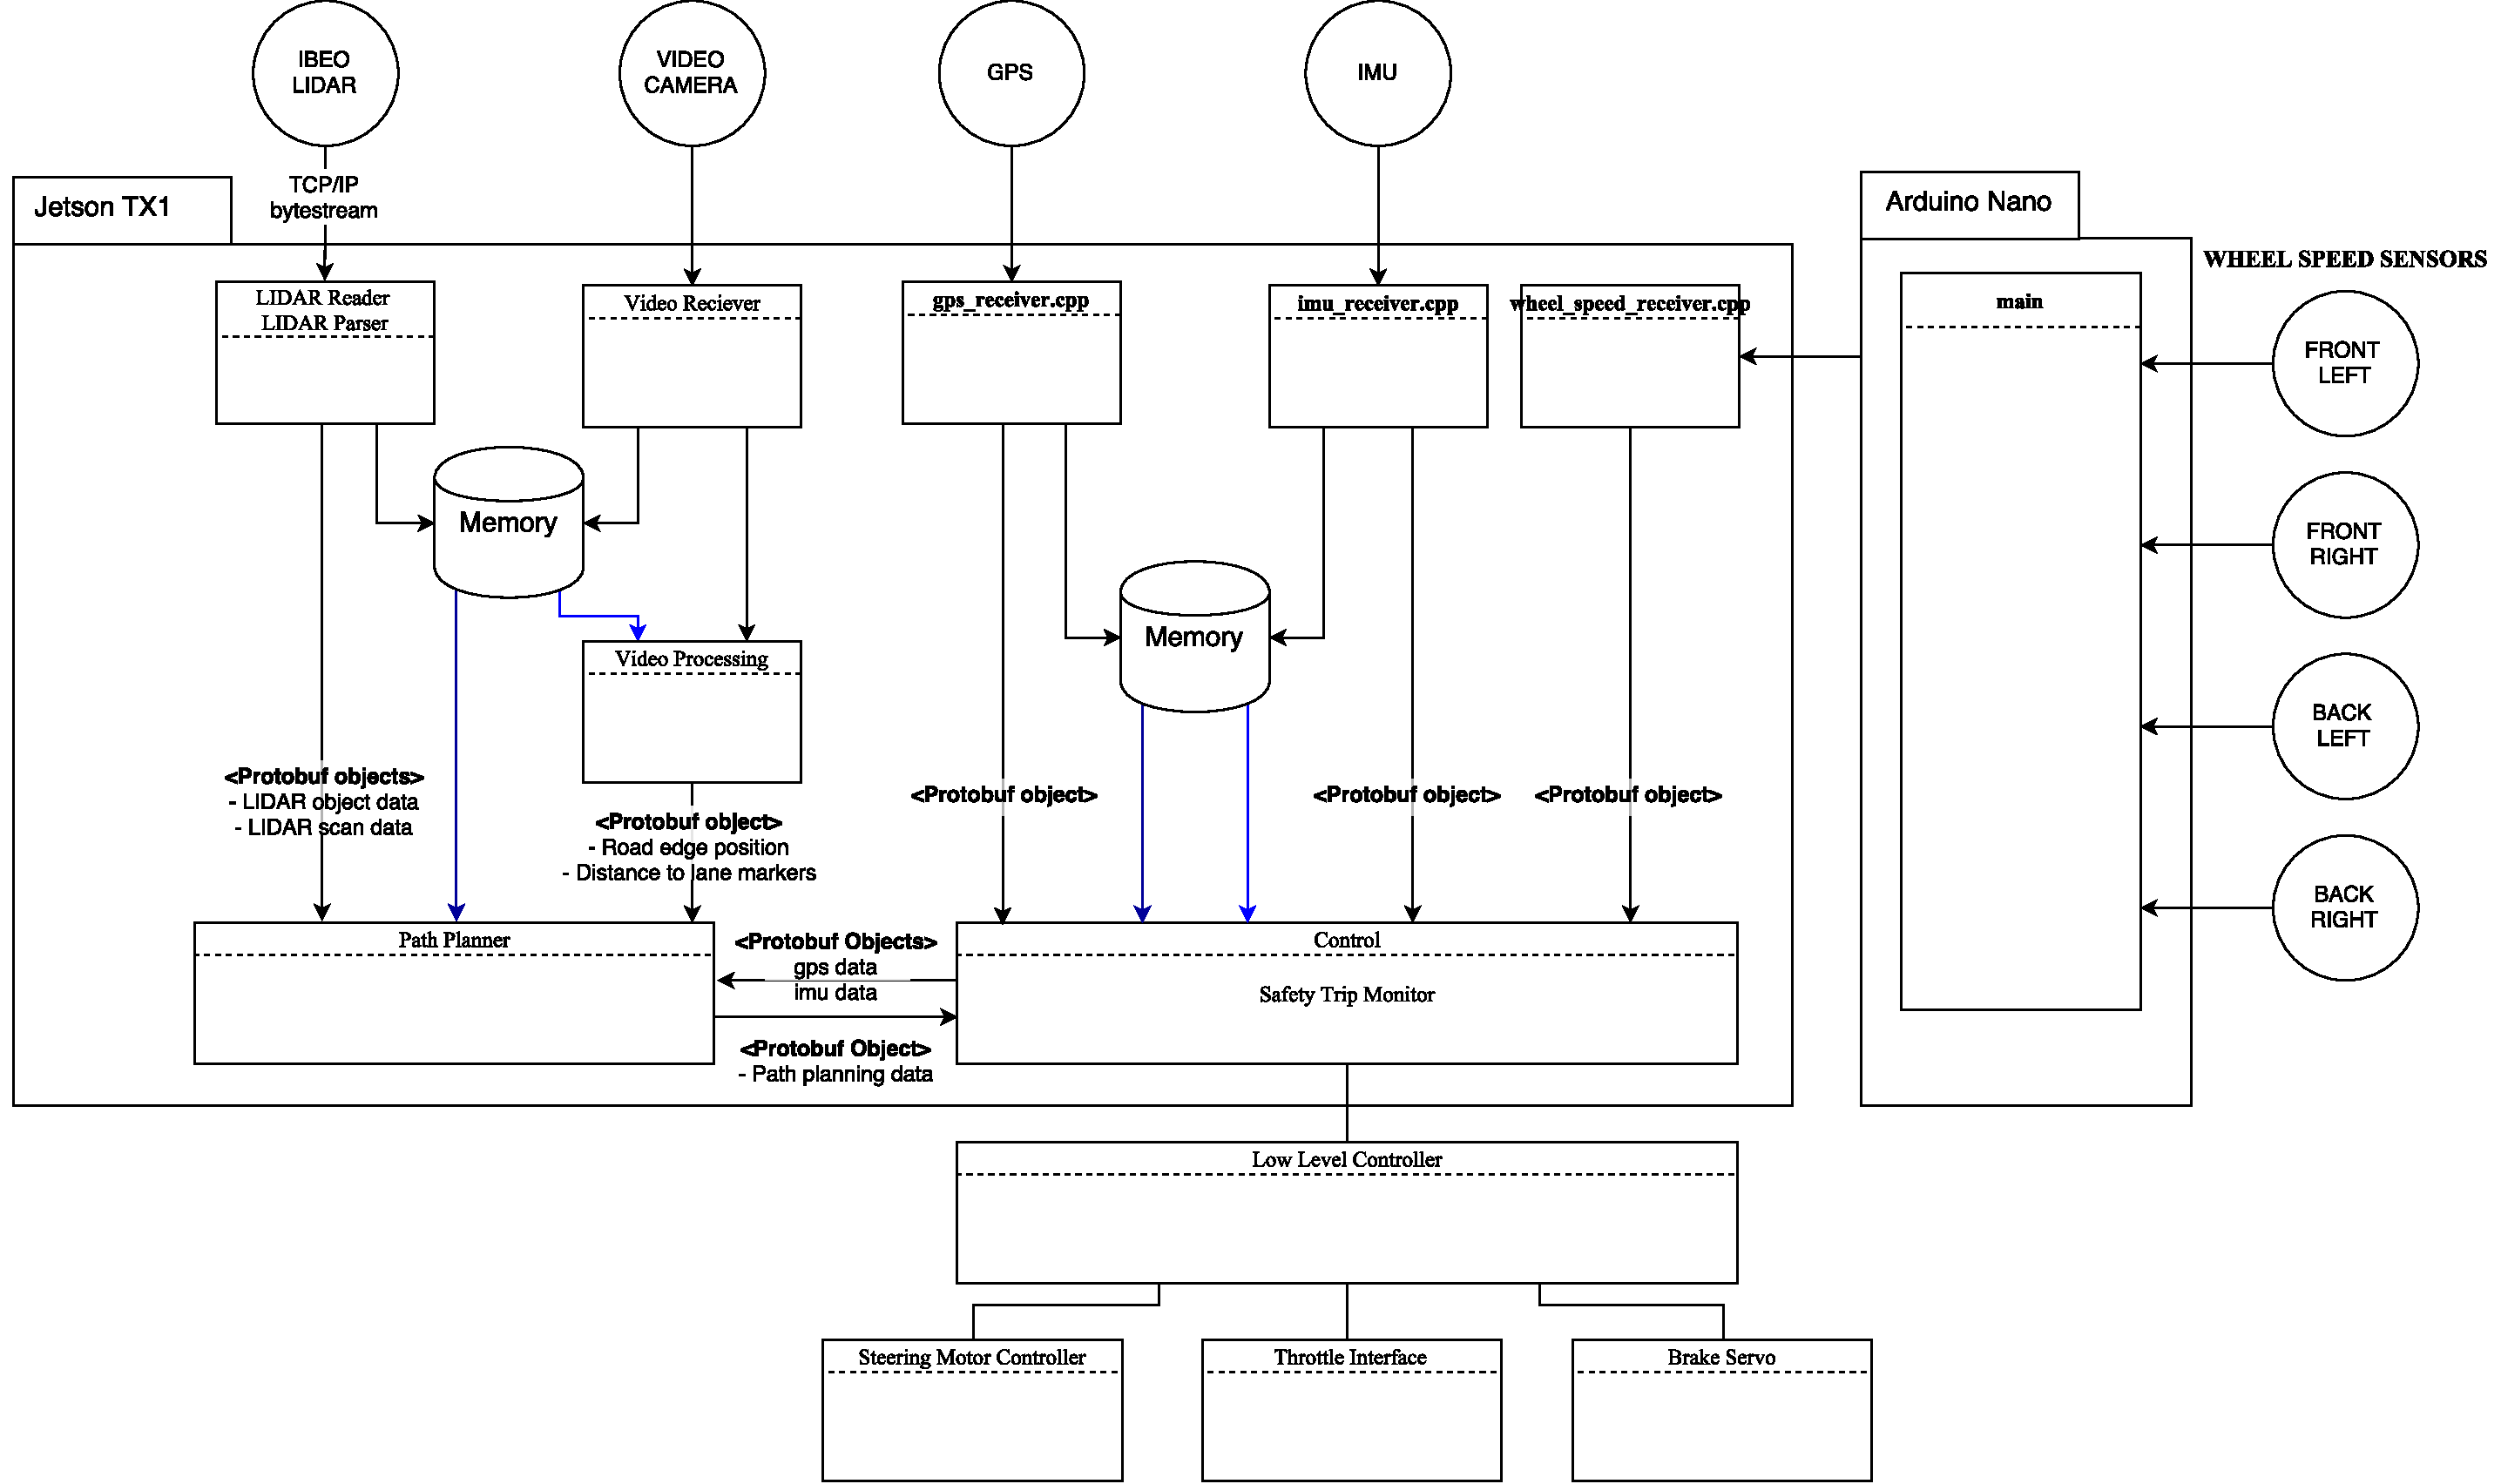
\includegraphics[width=\linewidth]{arch}
	\caption{Network architecture of REView.}
	\label{fig:9:arch}
\end{figure}

REView’s overall architecture can be summarised as Fig.~\ref{fig:9:arch}, consisting of seven components --- an EV server, charging station server, a solar downloader, data processing scripts, a database, a web server and its web interface. 

The charging stations and vehicles are all fitted with machine-to-machine (M2M) modems, which are perpetually connected to Telstra’s 3G Universal Mobile Telecommunications System (UMTS) network on the 850 MHz frequency. These modems then connect to our local server to transmit data over the Transmission Control Protocol (TCP) across two dedicated ports --- one for the charging stations and another for the vehicles, as the charging stations and vehicles package data through different protocols. The server handles these transmissions through a SocketServer framework on Python 2.6.

\nomenclature[z-umts]{UMTS}{Universal Mobile Telecommunications System}
\nomenclature[z-tcp]{TCP}{Transmission Control Protocol}

The Python daemons that run the SocketServer function receive and parse the incoming telemetry data from the charging stations and vehicles before appending these data onto a PostgreSQL database. This process also verifies data integrity and consistency by filtering any duplicates and non-events. This PostgreSQL database is installed onto the same server, which stores all data relating to telemetry, charging stations, vehicles and users. The platform’s Apache front end can then access this data for visualisation and analysis. 

The REView website features several pages including vehicle tracking, vehicle statistics, charging station status, charging station statistics, billing, heat maps, journey lists, charging lists, mobile tracking, and more. Depending on the type of user (station operator, station user or EV tracker) some pages are restricted or hidden. The website is a secure HTML 5 site with live information, interactive maps, graphs and customisable time scales. The supported browsers are Chrome, Microsoft Edge, Firefox and Safari, allowing access from computers, tablets and smartphones. At the time of writing, we are running PostgreSQL 8.4.20 and Apache 2.2.15 on a Red Hat Enterprise Linux (REHL) 6.10 server platform.

\nomenclature[z-rehl]{REHL}{Red Hat Enterprise Linux}

\section{Charging Infrastructures}
\label{sec:9:charging}
Our charging station network was established in 2011 as part of our research initiatives into the Western Australian EV landscape, which enables the collection of charging data to quantify charging trends and behaviours. This began with the installation of the Level 2 AC stations in the Perth metro area, followed by the installation of the 50 kW DC fast-charging station at UWA in 2014. We offer these charging stations free of charge to EV owners in return for research and data collection. The AC and DC stations transmit data through different protocols but are monitored for the same information. In other words, we collect information pertaining to charge times, duration and energy consumption from the stations for data visualisation and modelling. The following subsections detail the functions of these charging stations.

\subsection{DC Charging}
The 50 kW DC fast-charging station at UWA is a Tritium Veefil-RT~\cite{tritium_pty_ltd_veefil-rt_nodate} (see Fig.~\ref{fig:9:dccs}), which supports charging over the CHAdeMO~\cite{anegawa_development_2010} and SAE Combined Charging System (CCS) Type 2 (IEC 62196-3)~\cite{commission_iec_2014} standards. This station performs telemetry through the Open Charge Point Protocol (OCPP) 1.6 over a 3G UMTS network. Data from the station is first pushed onto Tritium’s server before it is pushed back to our local server, this allows Tritium to collect and consolidate data from its charging stations, and to streamline their maintenance and support on the station. The simplified class diagram in Fig.~\ref{fig:9:umldc} summarises REView’s functions on the DC station.

\nomenclature[z-ccs]{CCS}{Combined Charging System}
\nomenclature[z-iec]{IEC}{International Electrotechnical Commission}

\begin{figure}[H]
	\centering
	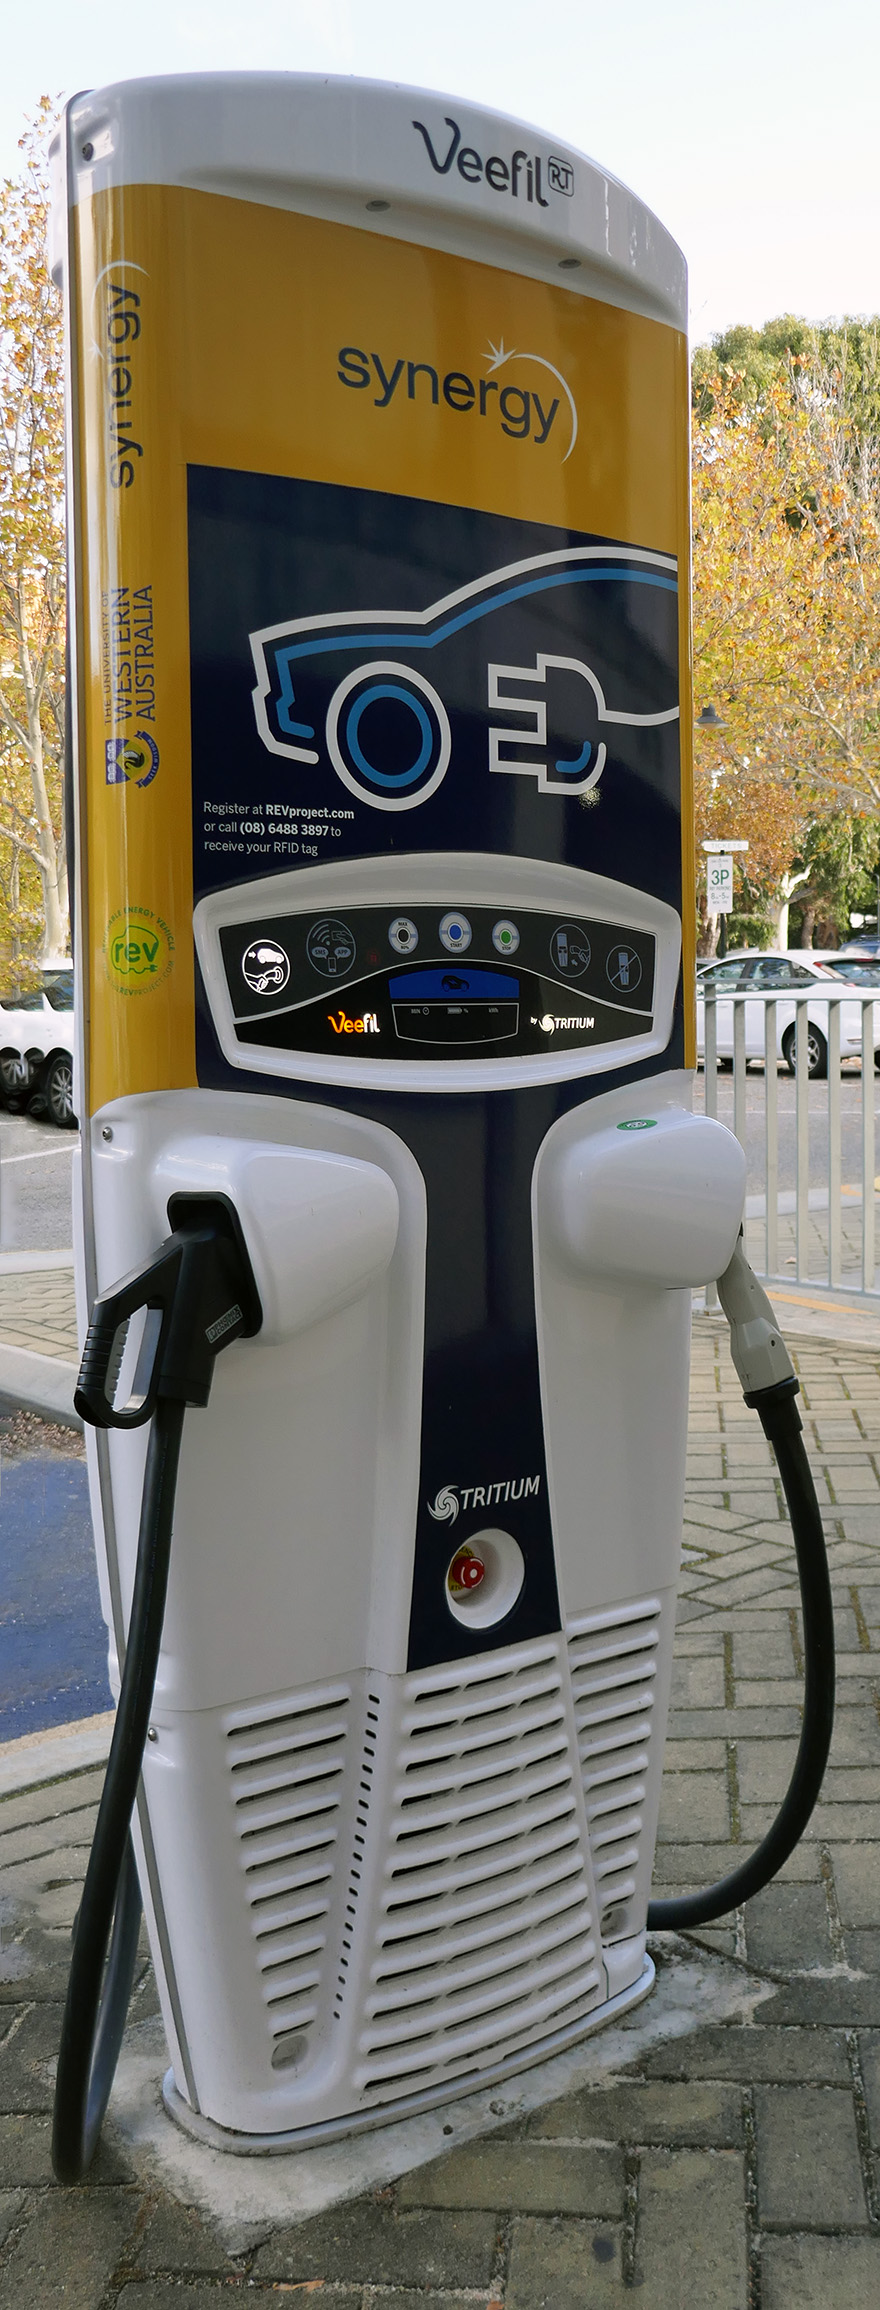
\includegraphics[width=0.2\linewidth]{dc-cs-cropped}
	\caption{UWA’s Tritium Veefil-RT DC fast charging station.}
	\label{fig:9:dccs}
\end{figure}

\begin{figure}[H]
	\centering
	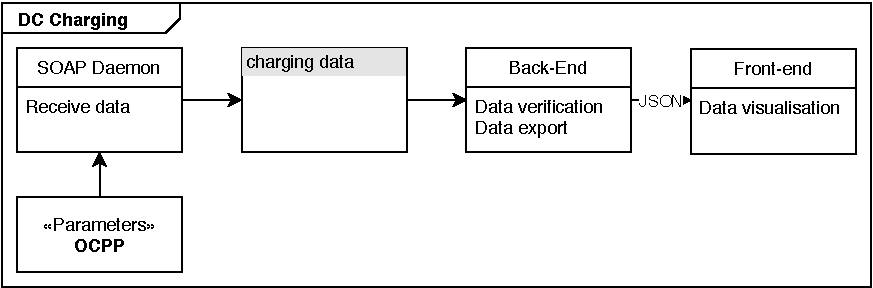
\includegraphics[width=\linewidth]{uml-dc}
	\caption{Simplified class diagram of REView’s DC station management.}
	\label{fig:9:umldc}
\end{figure}

\subsubsection{Communication Protocols}
OCPP data from Tritium’s servers are transmitted through the Simple Object Access Protocol (SOAP). We run a PHP SOAP server with its service functionality described in a Web Service Description Language (WSDL) file, following the service list as described by e-laad.nl~\cite{elaadnl_elaad_nodate}, to which we have ensured its compatibility with the Veefil charging stations. The charging station constantly transmits timestamped SOAP messages relating to heartbeats, start/stop charging events, status notifications, user authorisation and energy meter values.

\nomenclature[z-soap]{SOAP}{Simple Object Access Protocol}
\nomenclature[z-wsdl]{WSDL}{Web Service Description Language}

By referencing the WSDL file, our SOAP server receives and logs incoming data, subsequently appending it into the dccharge table. Each charging station user is assigned a unique identification (ID) the charging vehicle, and each station broadcasts a unique station ID that corresponds to its installed location; for each charging event, the charging station measures energy consumption in Wh units, along with its start and end times; finally, the station also broadcasts the charging standard used (CHAdeMO or CCS2) for each charging event.

\nomenclature[z-id]{ID}{Identification}

From the series of SOAP messages, the server appends charge data following Algorithm~\ref{algo:9:dccharge}.
The combination of this data allows us to perform time series analysis and modelling with regards to charge frequencies, duration, energy consumption and charge standard used. Additionally, we have instigated measures to maximise user participation through the station’s proximity to the city centre, while providing the service free of charge. These measures provide us with reliable data to model EV trends and fast-charging behaviours around Perth.

\begin{algorithm}[H]
	\begin{flushleft}
		\caption{DC charges database append}\label{algo:9:dccharge}
		\begin{algorithmic}[1]
			\Procedure{DCAppend}{incoming header}
			\State open Connection to database and table \textit{dccharge}\
			\State read incoming header
			\If{header is \textit{StartTransaction}}
			\State append to \textit{dccharge} with values \textit{TransactionID}, \textit{UserID}, \textit{StationID}, \hspace*{12.5mm}\textit{StartTimestamp}, \textit{StartUnits}, \textit{ConnectorID}\
			\EndIf
			\If{header is \textit{StopTransaction}}
			\State update \textit{dccharge} with values \textit{UserID}, \textit{StopTimestamp}, 
			\textit{StopUnits}, \hspace*{12.5mm}\textit{TransactionData} where same \textit{TransactionID}
			\State update \textit{status} = ChargeComplete
			\EndIf
			\State close Connection to database\
			\EndProcedure
		\end{algorithmic}
	\end{flushleft}
\end{algorithm}

\subsubsection{User Authentication}
To improve data integrity, our DC station supports user authentication based on near-field communication (NFC). Users are given the flexibility to use any compatible NFC card in their possession, including those for public transportation, work or school. Fig.~\ref{fig:9:tagdc} shows a non-exhaustive example of NFC cards that the station accepts. The charging station reads these cards for a four-byte unique identification number (UID), which is presented as eight hexadecimal numbers. The UID is then crosschecked with its database entry for charging authentication. In addition to the tag number, users are required to register with UWA for their names, email, vehicle model and registration number; whereby these fields are stored in a separate table in the database.

\begin{figure}[H]
	\centering
	
\includegraphics[width=0.7\linewidth]{tag-dc}
	\caption[RFID cards supported by the DC station]{RFID cards supported by the DC station. Pictured are a Transperth Smart-Rider card, a UWA Student ID and a general issue MIFARE RFID card, commonly used by station users.}
	\label{fig:9:tagdc}
\end{figure}

\nomenclature[z-rfid]{RFID}{Radio-frequency identification}

\subsubsection{Data Visualisation}
\label{sec:9:dcvis}
Data visualisation for the DC stations is performed through a series of SQL queries which are parsed through a series of JSON encode/decode processes over PHP. REView visualises these data in the form of time series graphs and pie charts, as well as a page delimited table with the option for a \textit{*.csv} file export.

\nomenclature[z-json]{JSON}{JavaScript Object Notation}

A back-end PHP script performs data parsing by connecting to the PostgreSQL database, which we use to send SQL queries. For the visualisation of charts, these arrays are appended with their headers, and then combined with chart parameters such as graph types, chart title, axes titles and legends; which are subsequently encoded into a JSON representation. For a table visualisation, the JSON representation will also include the total number of charging events to enable the page delimiter to determine the number of pages for the table.

Likewise, a front-end PHP script \textit{gets} the JSON representations from the back-end script and decodes it. This script interfaces with the web browser and is therefore also programmed with HTML and JavaScript as a webpage. Users of this webpage can specify visualisation periods with a start and end date, which is then used as part of the SQL statement to generate the query. The front-end script then parses the decoded JSON representation to determine all chart parameters, and subsequently plots them in a table using the Google Visualisation API~\cite{google_developers_google_nodate} as illustrated in Fig.~\ref{fig:9:dcvis}.

\begin{figure}[H]
	\centering
	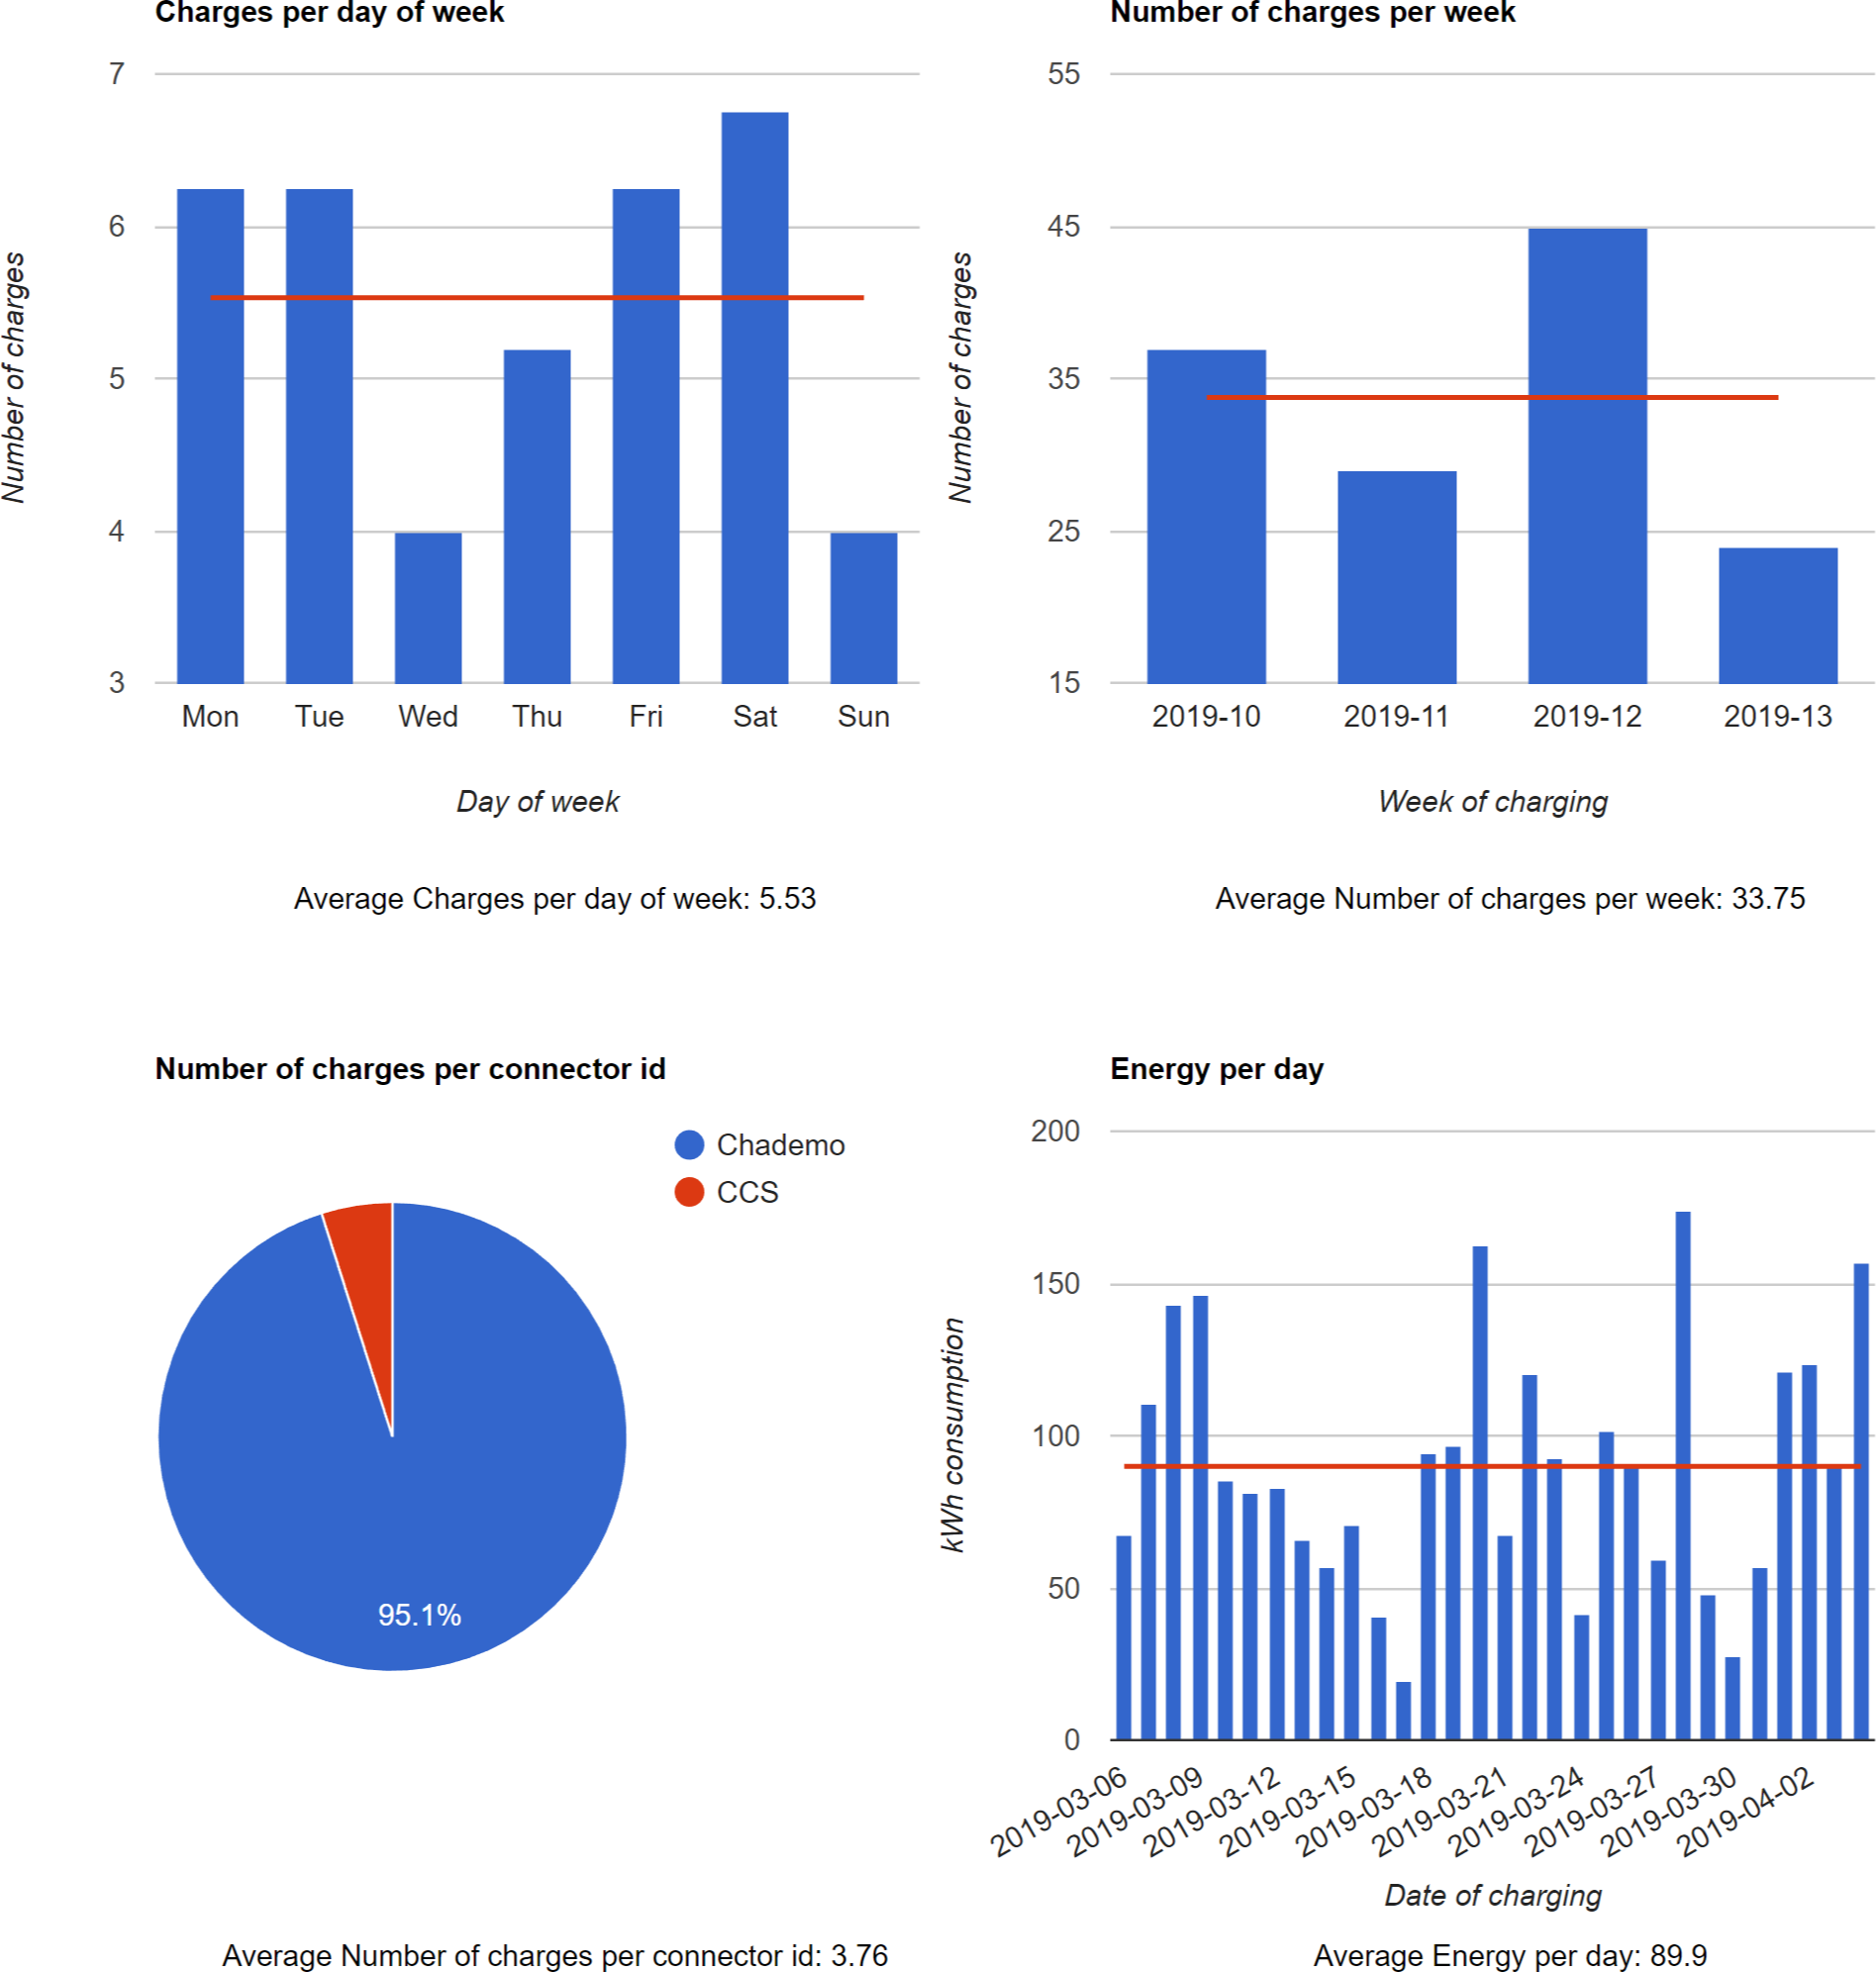
\includegraphics[width=\linewidth]{dc-vis-crop}
	\caption[Examples of visualisations for the DC station]{Examples of visualisations for the DC station given the month ending 5 April 2019.}
	\label{fig:9:dcvis}
\end{figure}

On the other hand, the table visualisation front end as illustrated in Fig.~\ref{fig:9:dctbl} draws an HTML table and fills it with the array obtained from a query that returns data from all DC charging events with the columns storing start and end times, charge duration, energy consumption and type of connector used. Each page is limited to 50 entries as defined in the query. This page supports \textit{*.csv} data exports, whereby the file will be downloaded with the same table headers.

\begin{figure}[H]
	\centering
	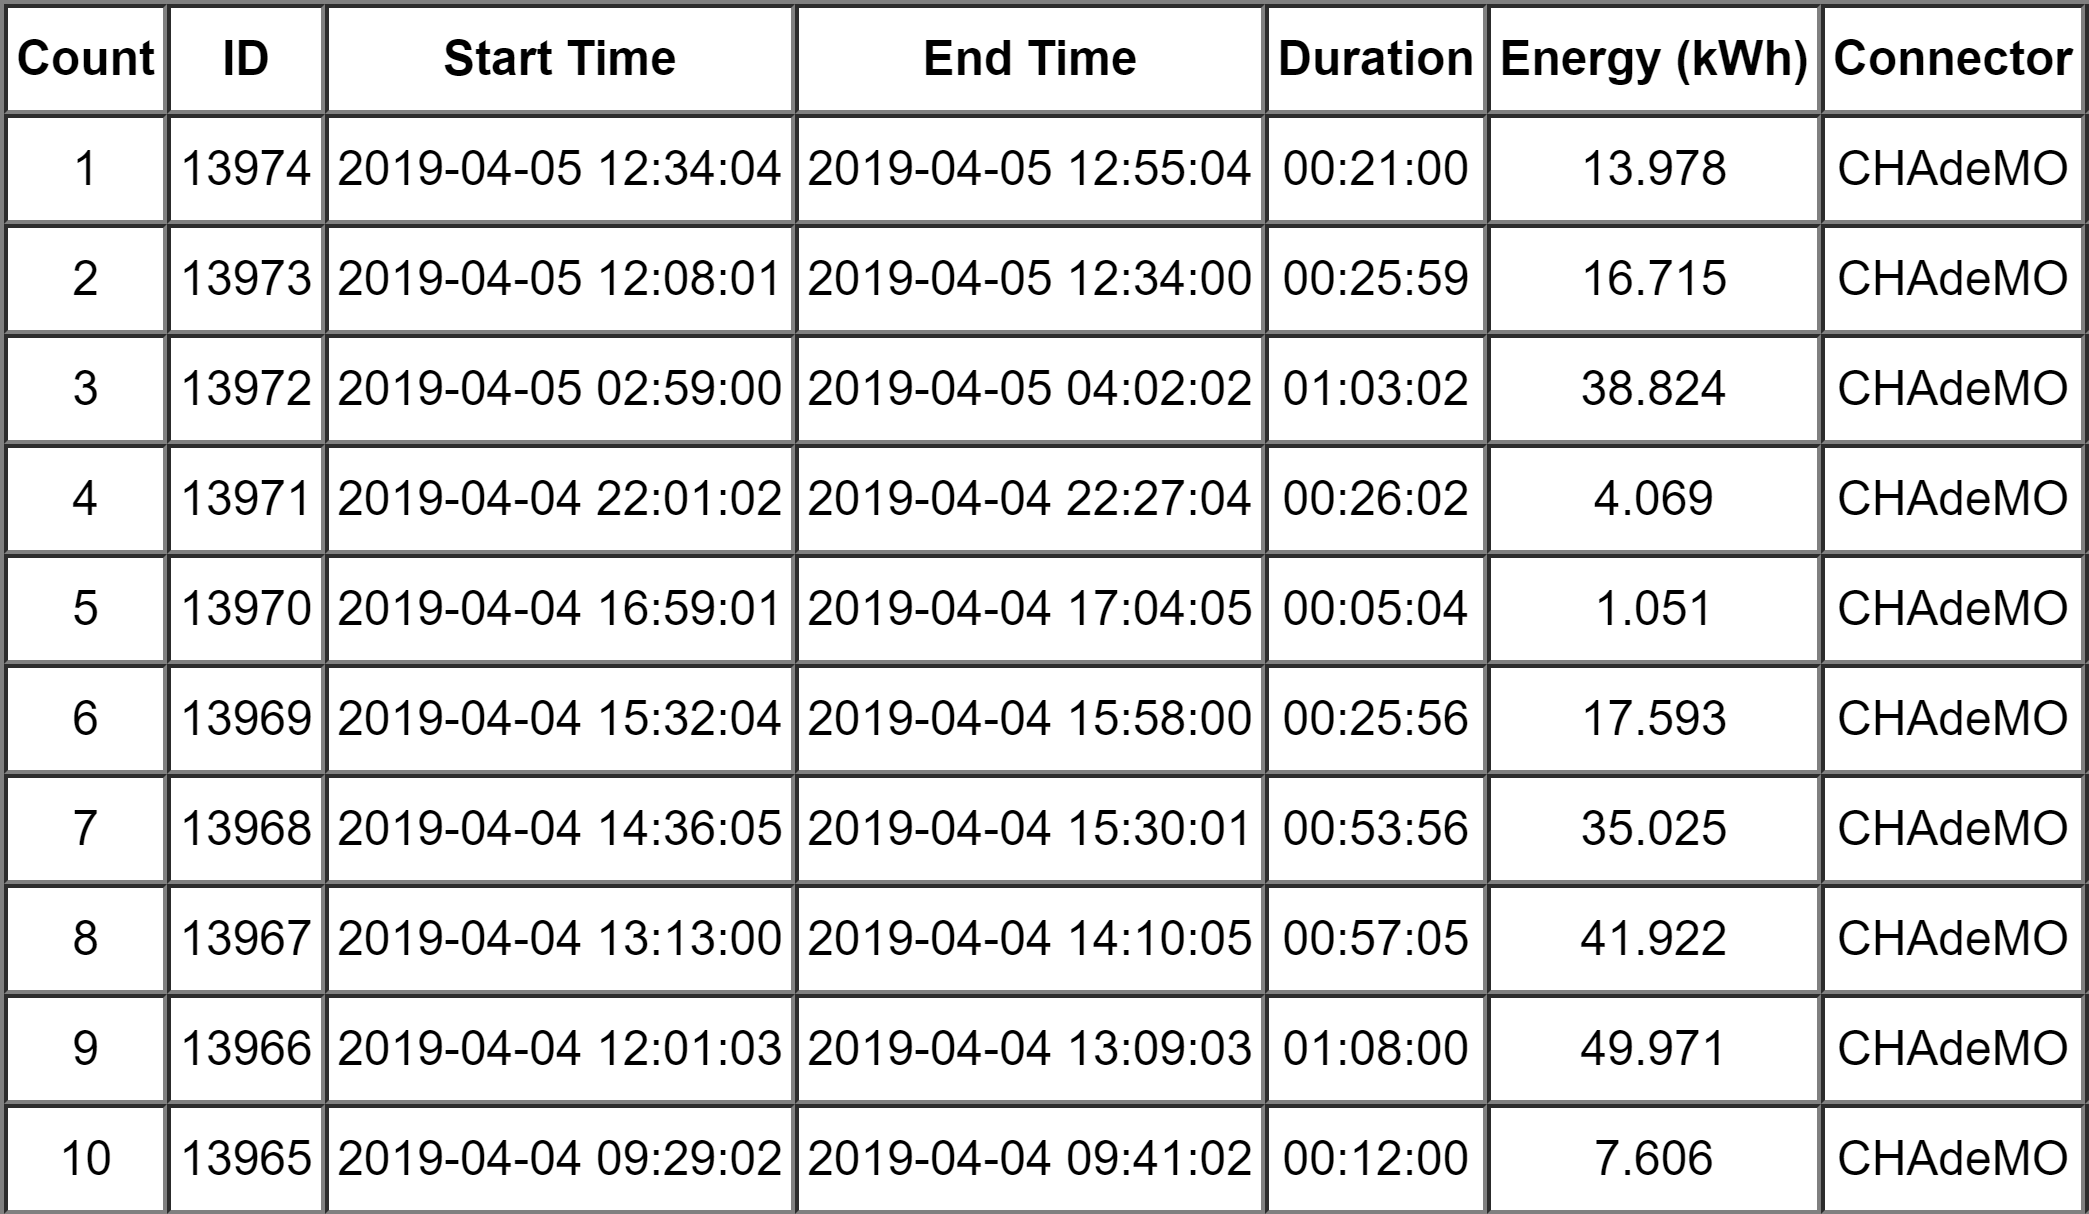
\includegraphics[width=0.8\linewidth]{dc-table-crop}
	\caption[DC charges table]{Screen grab showing the DC charges table on REView with the last ten charges.}
	\label{fig:9:dctbl}
\end{figure}

\subsection{AC Charging}
Our AC charging station network consist of 11 dual outlet (see Fig.~\ref{fig:9:accs}) and one single outlet Elektromotive Elektrobay charging stations, totalling 23 stations. These charging stations act as individual clients and connect to a central server node in a many-to-one configuration. Each charging station is powered through a 7 kW three-phase AC supply and are either wall mounted or floor mounted. The charging outlets support the IEC 62196-2 (Type 2/Mennekes) standard, which is compatible with all recent EVs sold in Australia. The stations are water resistant and fitted with overcurrent protection and RCD switches. The functions of REView on our network are as summarised in the simplified class diagram in Fig.~\ref{fig:9:umlac}, and are elaborated in the respective subsections.

\nomenclature[z-rcd]{RCD}{Residual-current device}

\begin{figure}[H]
	\centering
	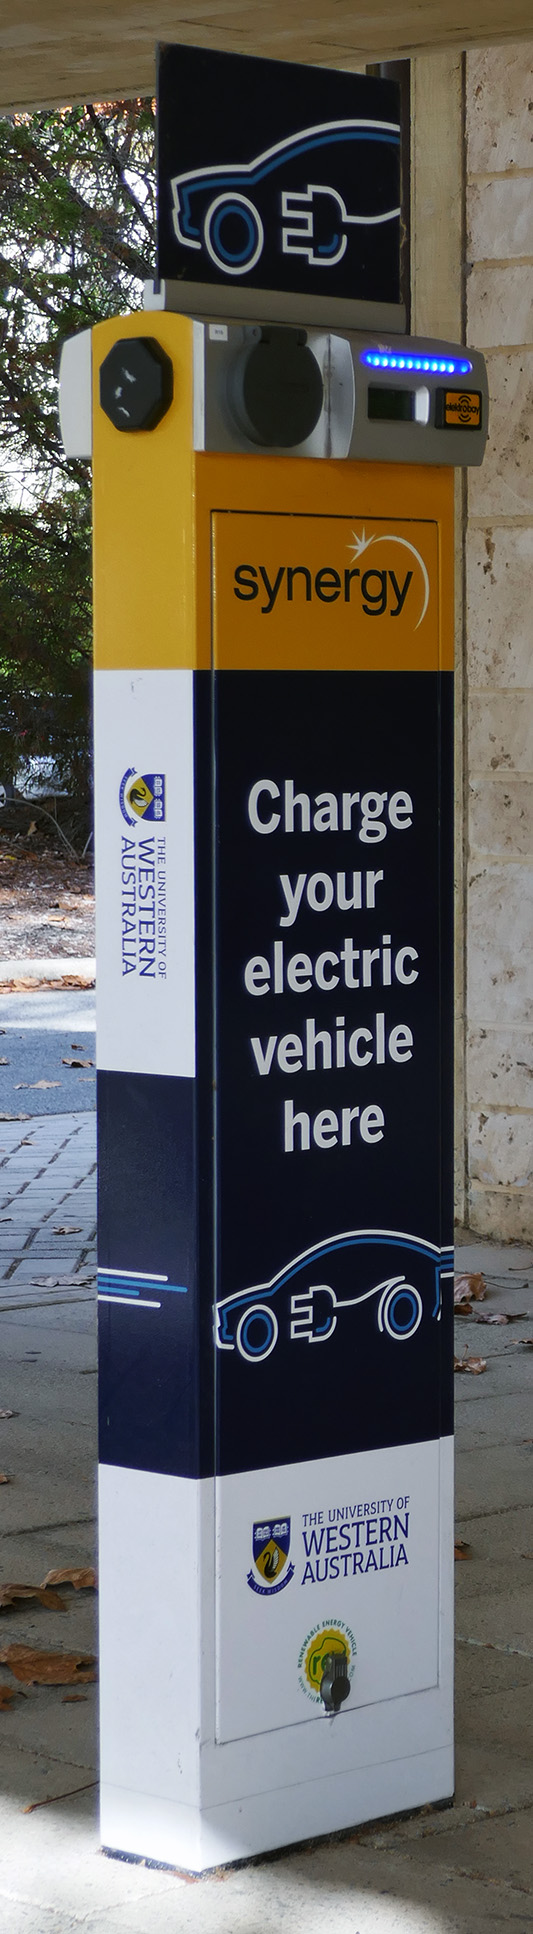
\includegraphics[width=0.17\linewidth]{ac-cs-cropped}
	\caption{UWA’s dual outlet Elektromotive Elektrobay AC charging station.}
	\label{fig:9:accs}
\end{figure}

\begin{figure}[H]
	\centering
	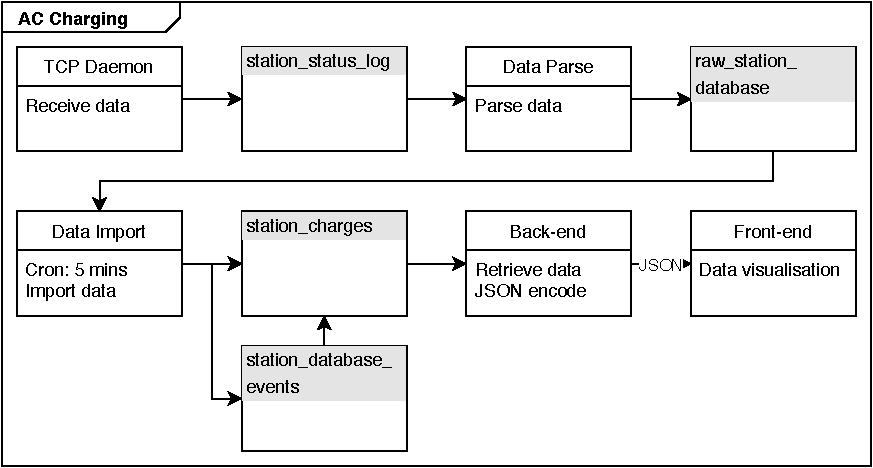
\includegraphics[width=\linewidth]{uml-ac}
	\caption{Simplified class diagram showing REView’s AC station management.}
	\label{fig:9:umlac}
\end{figure}

\subsubsection{Communication Protocols}
The AC station network achieves telemetry through the RS-232 serial standard, wherein for each station, a DE-9 cable connects to a Four-Faith F2414~\cite{xiamen_four-faith_communication_technology_co._ltd._f2414_nodate} High-Speed Downlink Packet Access (HSDPA) M2M modem (see Fig.~\ref{fig:9:acmodem}), transmitting charging data directly to our local server. We configured these modems using AT Commands, which instructs them to connect to our server through its IP address and port number, using TCP for data transmission. These modems establish a perpetual cellular connection upon power on, enabling them to transmit data from the stations on demand. Unlike the DC station, each AC station can be configured directly using the Elektromotive EB Connect software to set station parameters such as authorisation control, energy metering, charge limits, charge event and energy tracking. It also gives the administrator the ability to remotely login to the station or disconnect a user or reset a station.  To allow this software to connect to the station, the server can open a Secure Shell (SSH) tunnel between the station and the administrator PC. This can be used to either remotely configure the station’s modem or the charging station itself. 

\nomenclature[z-hsdpa]{HSDPA}{High Speed Downlink Packet Access}
\nomenclature[z-ssh]{SSH}{Secure Shell}
\nomenclature[z-ip]{IP}{Internet Protocol}

\begin{figure}[H]
	\centering
	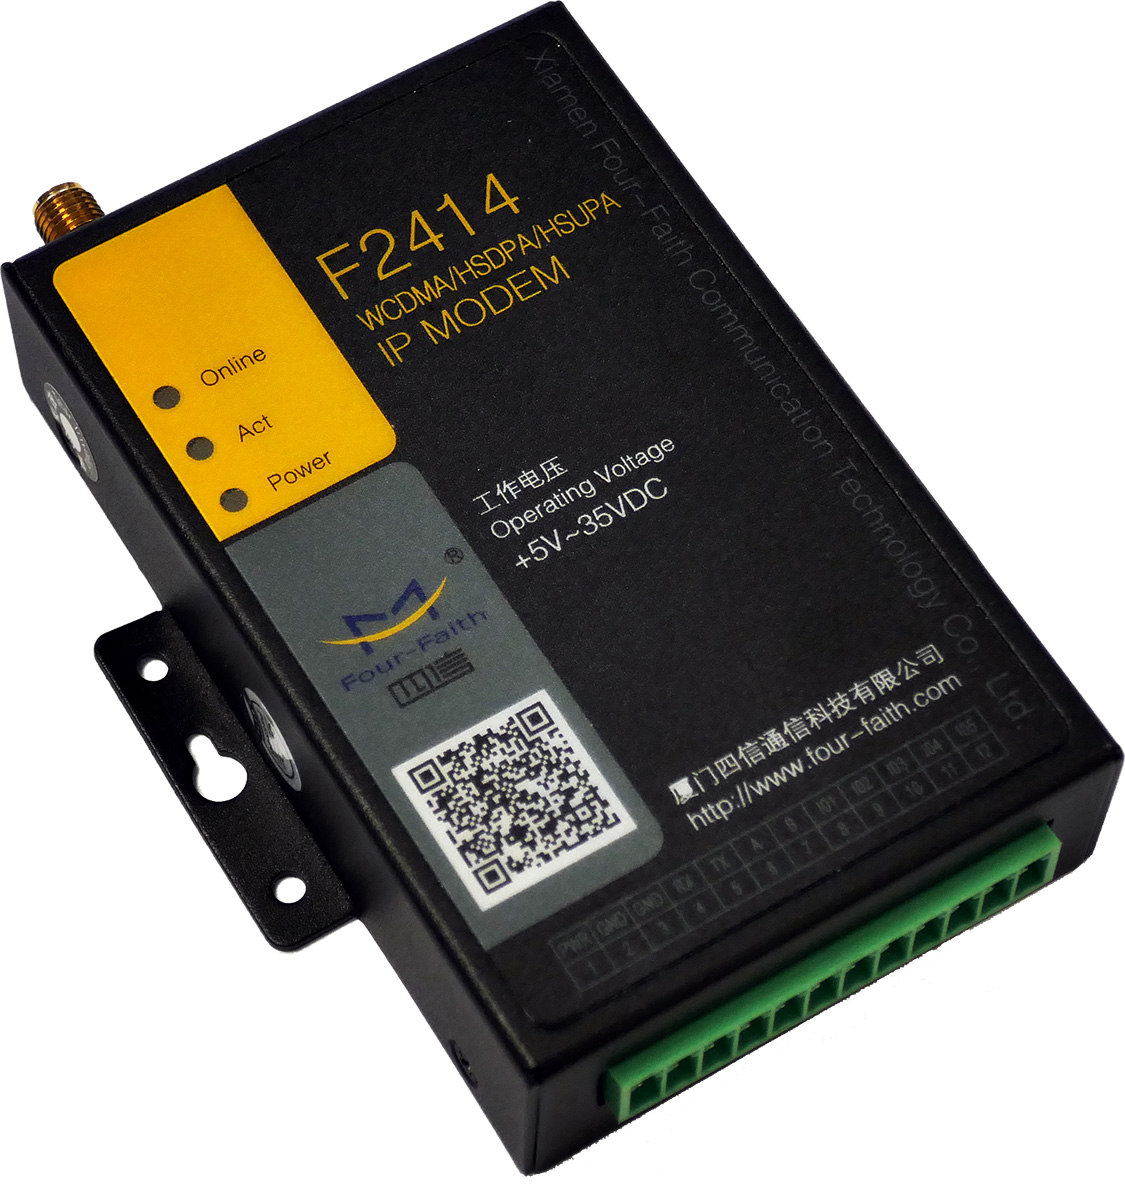
\includegraphics[width=0.4\linewidth]{f2414-rs}
	\caption{A Four-Faith F2414 M2M modem used in AC charging stations.}
	\label{fig:9:acmodem}
\end{figure}

Telemetry data from the AC charging stations follow Elektromotive’s proprietary protocol that transmits a series of concatenated, timestamped hexadecimal strings. In order to append the database, we run a Python-based data parsing script as a daemon that first splits the string into parts that correspond to the database variables, and then converts these parts into intelligible ASCII texts. This script logs all incoming telemetry data from the charging stations, which for every charging station, transmit at five-minute intervals. It also checks and sets the stations real time clock, and requests information from the stations internal database. 

\nomenclature[z-ascii]{ASCII}{American Standard Code for Information Interchange}

The charging station modems are configured to connect to the server, allowing them to use dynamically allocated IP addresses, which are generally a cheaper option to using more convenient static IPs. To distinguish the charging stations, each modem is programmed to transmit its Modem ID as a header for all outgoing TCP messages. The Modem ID is a four-byte alphanumerical variable that is appended into every database entry to uniquely identify the station and its charging outlet (left/right side). In other words, a dual outlet station will consist of two modems, one for each charging outlet. The server then parses all messages and groups them according to their charging stations based on this Modem ID.

Each station keeps a record of several types of events, including charging, disconnect, power failure and reset. When the number of recorded events at the server is less than that at the station, the excess records are downloaded and stored for later statistical analysis. 

\subsubsection{Telemetry Parameters}
In addition to the Modem ID, other relevant parameters are further detailed in their respective paragraphs.

\paragraph{Clock}Each AC charging station keeps a clock which timestamps telemetry messages as they are produced. The stations’ clock differs from the server’s clock whereby the server’s clock is used to timestamp the telemetry messages as they are received. This clock redundancy is particularly useful at times when the UMTS network is unreliable, in which case the charging station will store these messages in memory before transmitting them in series as soon as the UMTS network re-establishes. While the charging stations’ clocks support over-the-air synchronisation, this process occurs intermittently on demand, which implies that the server’s clock, being consistently connected to the Internet, is more accurate. To accommodate this issue, the data parsing script checks for any time discrepancy between the server and the station, setting the message timestamp to the server’s time if it is less than 12 hours apart.

\paragraph{Station Attributes}A \textit{flag} variable transmits station attributes through an array of 16 binary objects that correspond to various station statuses. These array elements are, in sequence, “data erased”, “station restarted”, “no return timer activated”, “no power drain”, “excess power drain”, “power failure”, “door jammed”, “door forced open”, “record trip”, “mains status”, “door status”, “charge time exceeded”, “transaction start”, “transaction end”, “remote event”, and “force end charge cycle”. The values presented in this array are important for data collection and station diagnostics. For example, we use a combination of these station attribute flags to decipher station logs and append them as charging events into the database.

\paragraph{Station Status} The combination of short telemetry intervals with its contained station attributes enables REView to determine the status of each station, where they are classified as “In use”, “Not in use” or “Unknown”, and subsequently visualised on the front end for users to check on the station bays’ occupancy. While the “in use” and “not in use” states can be ascertained from the telemetry logs, an “unknown” state is set for a station when more than 15 minutes have elapsed since its last telemetry message was received, considering that each station is programmed to transmit messages every five minutes. A station that is “in use” will also display its current charging time and allowing registered users to track their charging status on their phones via a mobile website.

\subsubsection{User Authentication}
AC charging station users have been supplied with RFID tags for identification to allow monitoring and future billing. This also reduces the risk of cable theft, as only the correct tag can release the charging cable. Other identification methods used elsewhere include smartphone login, credit card swipe and in-vehicle identification, but these require higher security standards (in case of credit card readers) and constant Internet connection, which makes these methods more expensive.

\begin{figure}[H]
	\centering
	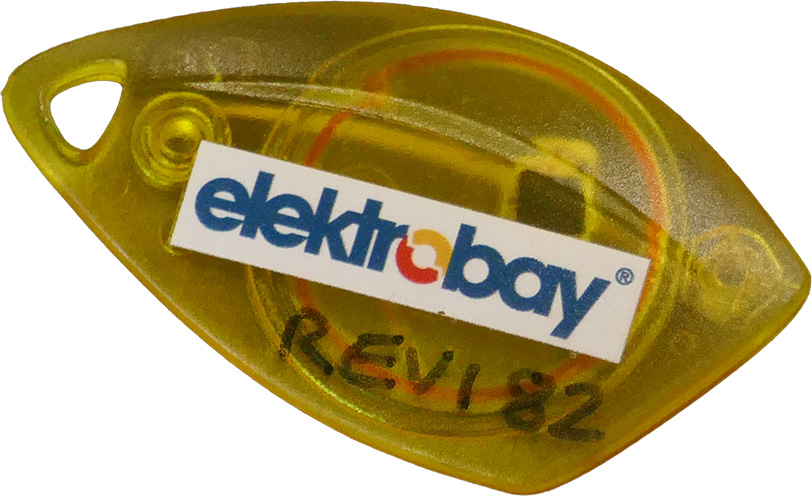
\includegraphics[width=0.35\linewidth]{tag}
	\caption[An RFID token used for our AC charging station network]{An RFID token used for our AC charging station network. Pictured here is the tag for the User ID REV182.}
	\label{fig:9:actag}
\end{figure}

User authentication on our AC charging station network is established through Elektromotive-supplied RFID tokens (see Fig.~\ref{fig:9:actag}). Each charging station is fitted with an RFID tag reader that conforms to the MIFARE DESFire~\cite{nxp_semiconductors_mifare_nodate} standard. These RFID tokens also communicate through the 13.56 MHz band and are also compatible with the DC charging station. Users intending to charge their vehicle at our charging station network are required to register their details and consent to having their charging data collected for research purposes. We issue the Electromotive RFID tokens to all registered users, and each RFID tag number uniquely identifies the user through the storing of the tag’s user ID.

\subsubsection{Database}
The database stores charging data from the charging station network in a normalised manner across three redundant tables shown in Figure 1.8, namely \texttt{raw\_station\_database}, \texttt{station\_database\_events} and \texttt{station\_charges}. This redundancy not only protects the data from accidental deletions, it also enables us to experiment and modify filter and merging rules for the tables while preserving data integrity. 

Noting the longer average charge duration of Level 2 stations (the location of AC stations sees most users leaving their vehicle charging while at work), we have set up REView to feature per-hour and per-day-of-week data recordings for charging duration and energy consumption. For instance, a size 24 array represents each hour of the day; a size 7 array represents each day of the week. By segregating these analyses into a time series, we can therefore visualise and model the stations’ utilisation as time progresses. The longer charge duration will often also imply that vehicles are left plugged into the charging stations even after they are fully charged. These vehicles are therefore subjected to a trickle charging state where their batteries are charged at their self-discharging rate, where the charging stations are \textbf{maintaining} charge at an \textbf{idle} state. To differentiate and analyse this charge maintaining state, we classify all charging instances that draw less than 1 kWh per hour as one that maintains charge, and that of more than 1 kWh per hour as one that is actively charging. 

We present Algorithms~\ref{algo:9:acimport1} and~\ref{algo:9:acimport2} for the importation of data between tables, each representing a different parsing script. 

\begin{algorithm}[H]
	\begin{flushleft}
		\caption{\texttt{station\_status\_log} to \texttt{raw\_station\_database}}\label{algo:9:acimport1}
		\begin{algorithmic}[1]
			\Procedure{ACAppend1}{incoming telemetry message}
			\State open Connection to database and table \textit{station\_status\_log}\
			\State read incoming \textit{NumRecords}, \textit{ModemID}\
			\State fetch lastEntry from \textit{station\_status\_log}\
			\While{incoming.\textit{NumRecords} $<$ lastEntry.\textit{NumRecords}}
			\State \textit{amount} = incoming.\textit{NumRecords} $-$ lastEntry.\textit{NumRecords}\
			\State fetch past \textit{amount} record from \textit{station\_status\_log}\
			\For{each \textit{amount} record}
			\State append into \textit{raw\_station\_database} with values \textit{StationID}, \textit{Flags}, \hspace*{18mm}\textit{ServerTime}, \textit{StationTime}, \textit{MeterReading}, \textit{EnergyReading}, \textit{Index}, \textit{UserID}, \hspace*{18mm}\textit{ModemID}
			\EndFor
			\EndWhile
			\State close Connection to table \textit{station\_status\_log}\
			\EndProcedure
		\end{algorithmic}
	\end{flushleft}
\end{algorithm}

\begin{algorithm}[H]
	\begin{flushleft}
		\caption{\texttt{raw\_station\_database} to \texttt{station\_charges}}\label{algo:9:acimport2}
		\begin{algorithmic}[1]
			\Procedure{ACAppend2}{incoming header}
			\State open Connection to database and table \textit{station\_database\_events}\
			\For{each \textit{ModemID} in \textit{station\_database\_events}}
			\State \textit{lastEvent} = max(\textit{endtime}) from \textit{station\_database\_events} at \textit{ModemID}
			\State get first \textit{event}
			\For{each \textit{event} where \textit{StartTime} $<$ \textit{lastEvent}}
			\If{not \textit{stationRestarted} and \textit{transactionStart} and \textit{serverTime} 
				$<$ \textit{currentTime} \hspace*{18mm}}
			\If{not \textit{chargeStart}}
			\State \textit{chargeStart} = \textit{event}
			\EndIf
			\State lastEvent = \textit{event}
			\EndIf
			\If{chargesStart and (transactionStart and transactionEnd) or 
				\hspace*{18mm}(chargeRestart and not transactionStart)}
			%\State \textit{duration} = \textit{EndTime} - \textit{StartTime}
			\State \textit{kWh} = \textit{EndMeterReading} - \textit{StartMeterReading}
			\State append into \textit{station\_database\_events} with values \textit{stationID}, \hspace*{25mm}\textit{StartTime}, \textit{EndTime}, \textit{kWh}, \textit{UserID}, \textit{rightSide}, \textit{ModemID}
			\EndIf
			\EndFor
			\State open Connection to table \textit{station\_charges}
			\For{each appended \textit{event}}
			\State append into \textit{station\_charges}
			\EndFor
			\EndFor
			\State close Connection to all tables and database
			\EndProcedure
		\end{algorithmic}
	\end{flushleft}
\end{algorithm}

We improve data integrity by setting charging limitations on the charging stations. These include a 12-hour charge duration limit, and an energy threshold between 3 Wh and 14.4 kWh. The charge duration limit ensures that users who forget to tag off after a charge, or subject their vehicles to extended periods of trickle charge are not accounted for data collection; similarly, current limits protect the charging stations from overloading and the charging event is properly terminated as soon as the vehicle’s battery is fully charged. On the database, we have programmed the data import script to filter for extremes and negative values. These filters ensure that 
\begin{enumerate}
	\item Energy values are between 0 kWh to 200 kWh. This upper limit is, at the time of writing, higher than the battery capacity of any commercially available EV.
	\item Charging durations are between 0 to 12 hours, to ensure that the charge duration limits are coherent with those set at the charging stations.
\end{enumerate}
Any entry that does not satisfy the filter boundaries are not imported into the \texttt{station\_charges} table.

\subsubsection{Data Visualisation}
Unlike the DC charging station’s architecture, data from the AC charging station network is stored entirely on the same local server and does not involve any communication between servers. Having all data eventually consolidated into a single table also enables us to condense, query and retrieve all data that is required for visualisation into a single SQL query that combines data from charging events with its tag owner. The result is encoded as a JSON representation that is subsequently sent to the front end that calls it.

Data visualisation at the front end is similar to the DC charging station’s whereby it generates a series of charts and a page delimited table. However, the added complexity of a charging station network, along with the increased variety of collectable data from it implies a differentiation from our descriptions in Section~\ref{sec:9:dcvis}. The Google Visualisation API is again used to render charts for the AC stations. The difference, however, is that data parsing is performed directly on a single SQL query result, as compared to sending multiple queries for the DC station. A JavaScript function is written to parse the decoded JSON representation and group them into multiple charts based on their headers. Users can select a specific time period for visualisation periods, as well as specific charging stations. In addition to time series charts describing energy usage and charge duration, having per-station and per-user data also enables cost patterns and energy usage to be visualised for each user and station in the form of pie charts. An example of these visualisations is given as Fig.~\ref{fig:9:acvis}.

\begin{figure}[H]
	\centering
	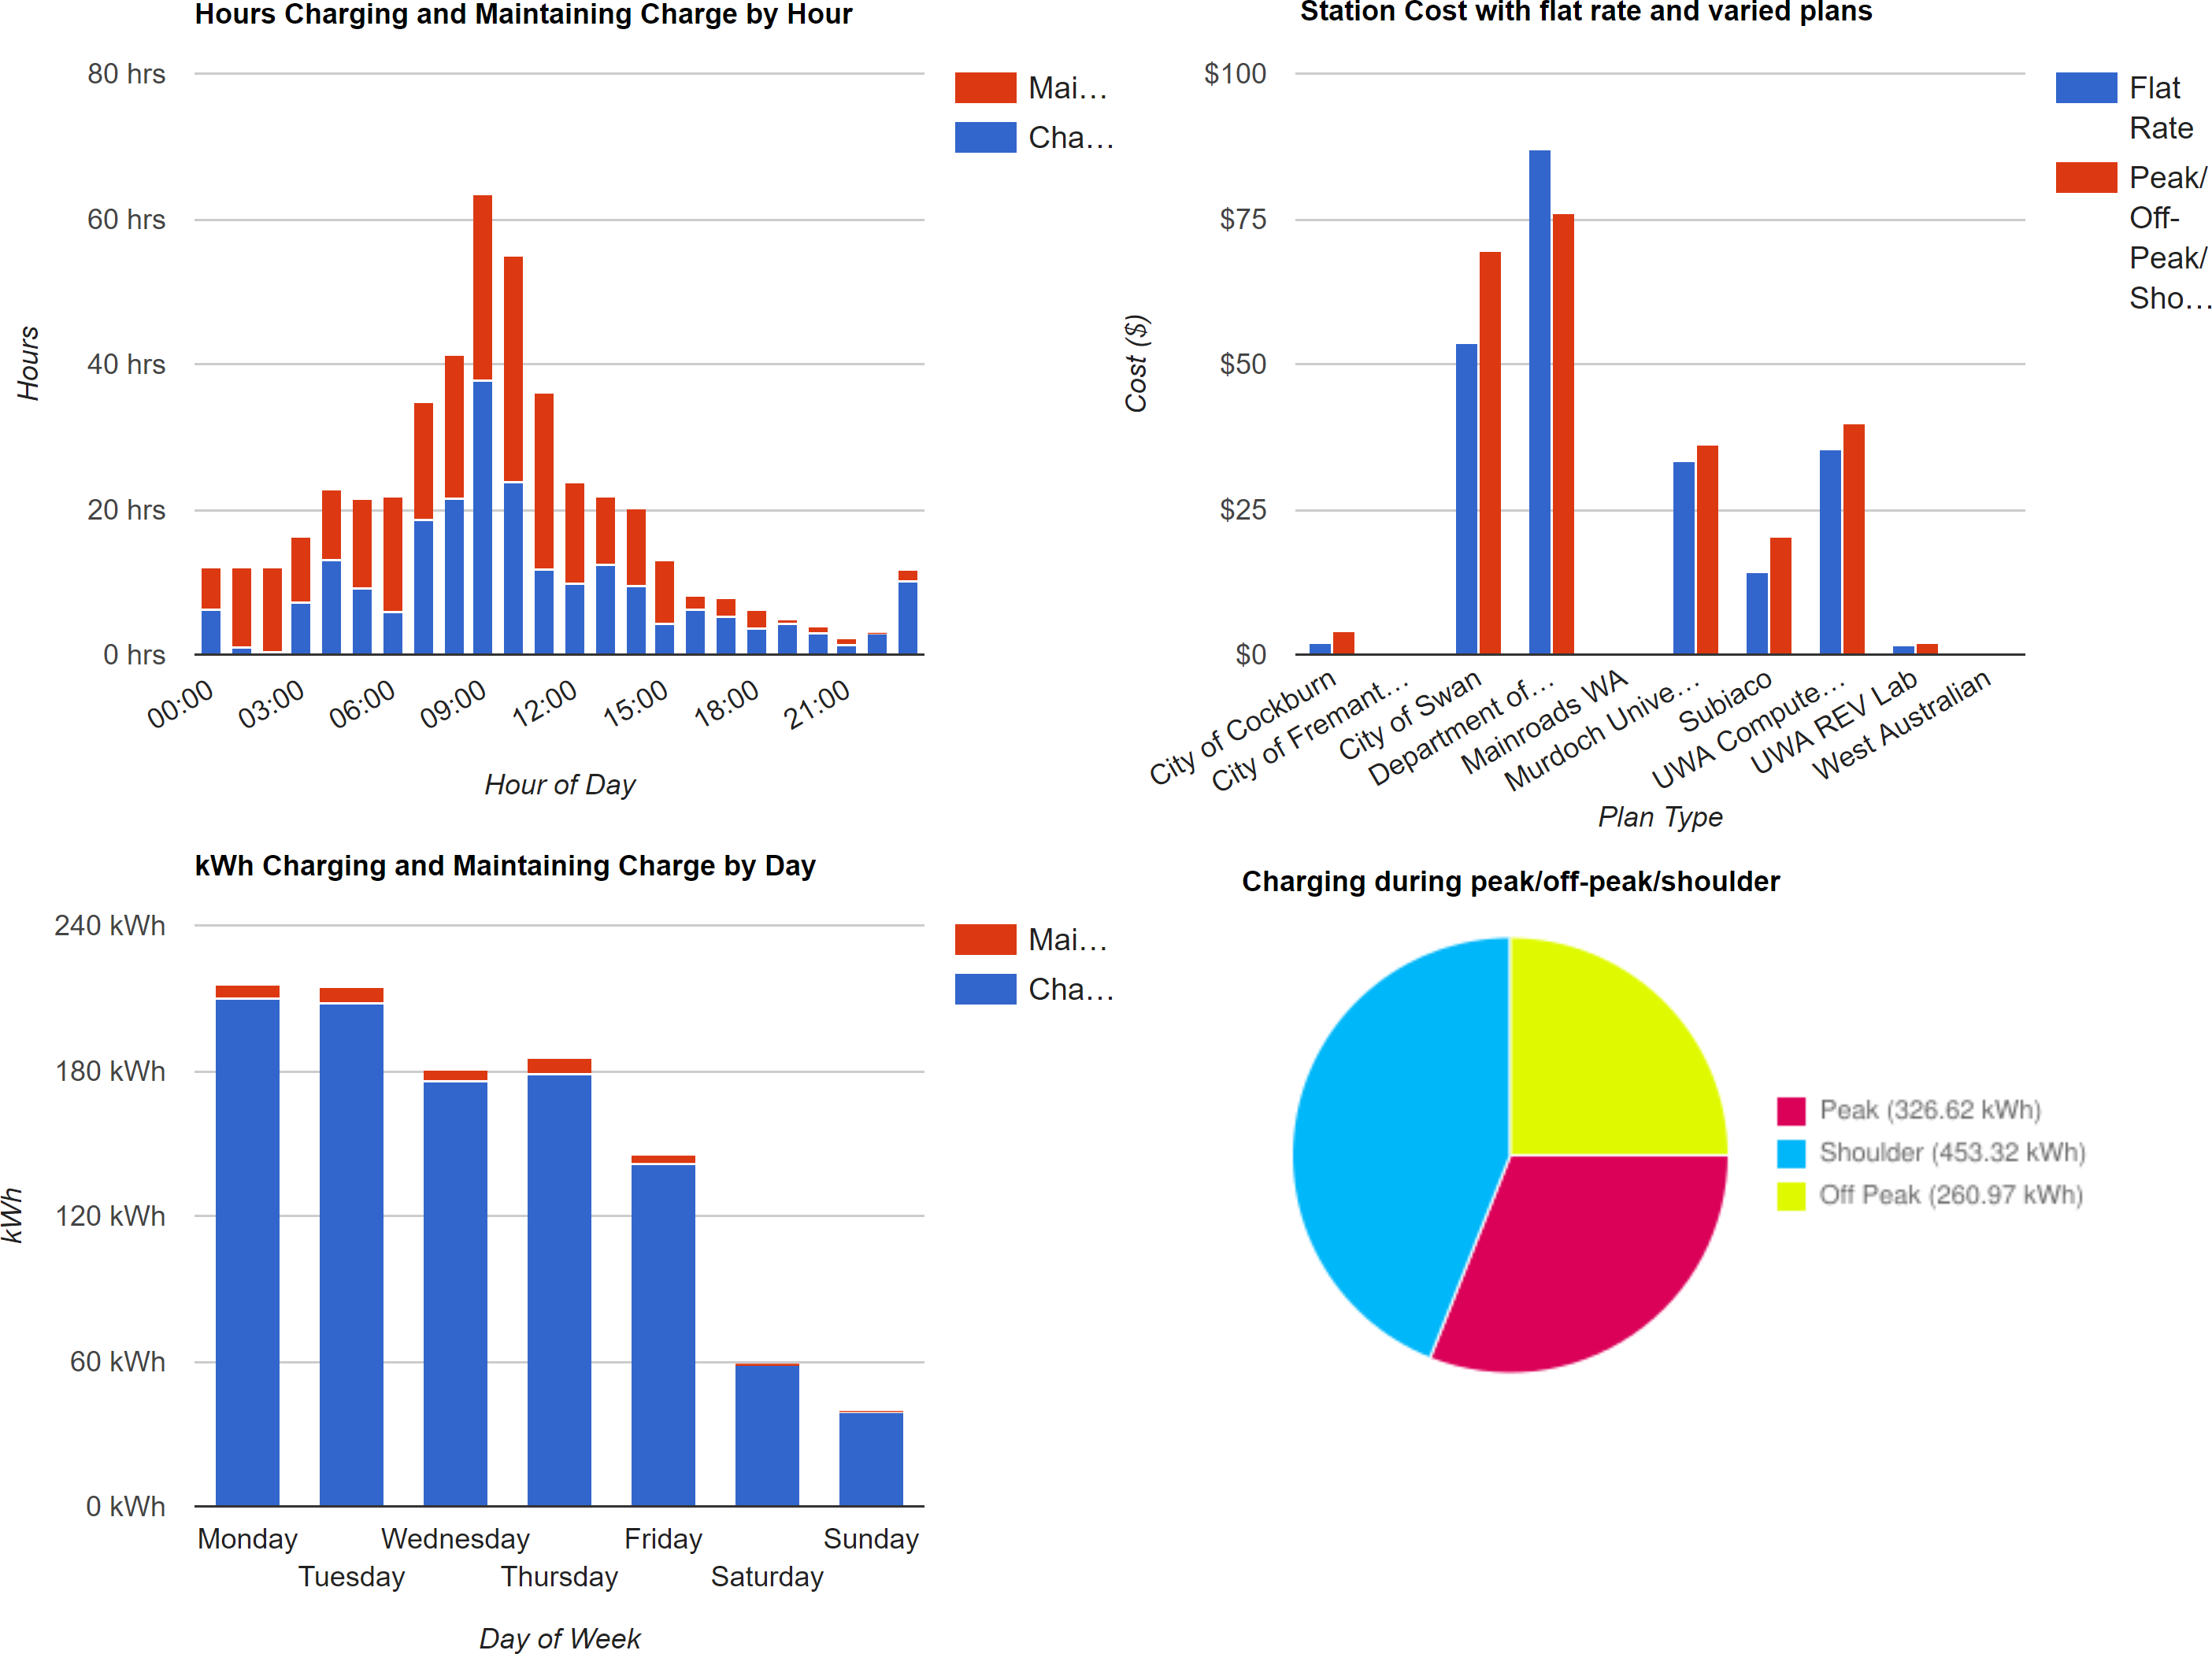
\includegraphics[width=\linewidth]{ac-vis-crop}
	\caption[Examples of visualisations for the AC station]{Visualisation examples for the AC stations given the month ending 5 April 2019.}
	\label{fig:9:acvis}
\end{figure}

Furthermore, using this query approach along with a visualisation period selection enables the front end to include a summary table for each charging station and its network. This table summarises, for any selected period, its total energy consumption, estimated running cost (peak and off peak), number of charges, total plugged-in time, total charging and maintaining charge time, average charge duration, average charging and maintaining charge duration, percentage of time in use and power used for peak, shoulder and off-peak times. Each of the statistics generated is useful to charging station operators.  The table shows:
\begin{itemize}
	\item Which electricity plan is more useful, displaying the cost of a flat rate of electricity price (e.g. 21.87¢ per kWh) and a tiered rate (peak/shoulder/off-peak, e.g. 42.15¢, 21.44¢ and 11.32¢ per kWh respectively), which charges more during peak times and less during off-peak times.
	\item Time spent charging the vehicle (drawing more than 1 kW) and the time spent plugged in and not charging as a percentage. This shows if a station is more used for charging or if a location is more used as a parking spot. 
	\item Time spent on a transaction (how long the vehicle is plugged in on average).
	\item Amount of time the station is actually in use versus its total time installed. Showing how often the stations are utilised as an average over all locations.
\end{itemize}

\section{Vehicle Monitoring}
\label{sec:9:vm}
REView’s electric vehicle tracking functionality was first established and presented as part of The REV Project’s WA Electric Vehicle trial in 2011, whereby a fleet of 11 electric-converted Ford Focuses were fitted with mobile GPS tracking units, which tracks the vehicles’ movement patterns, battery level, charging, headlight, heater, air conditioning and ignition status. 2.7 million data points were collected over the trial period, which includes 5,000 independent journeys averaging 9.3 km per trip and 1,600 charges. Since then, our vehicle tracking platform has expanded to include our electric Jet Ski, electric boat and autonomous driving projects. The incorporating of EV tracking onto REView enables us to better analyse usage behaviours of EVs and to model future commute habits. Results stemming from our vehicle tracking system are published in~\cite{speidel_analysis_2012}. Vehicle tracking on REView is performed according to the class diagram in Fig.~\ref{fig:9:umlvt}, and is detailed in the subsections.

\begin{figure}[H]
	\centering
	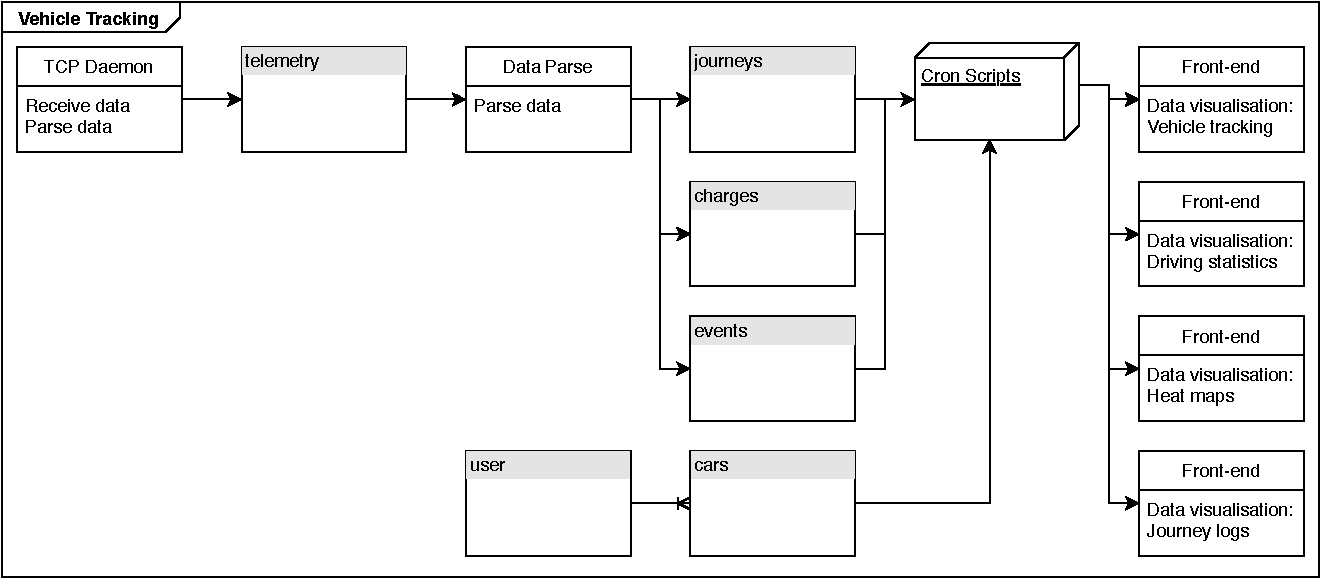
\includegraphics[width=\linewidth]{uml-vt}
	\caption{Simplified class diagram showing REView’s vehicle tracking system.}
	\label{fig:9:umlvt}
\end{figure}

\subsection{Communication Protocols}
Our fleet network was initially fitted with Astra Telematics’ AT110~\cite{astra_telematics_limited_at110_nodate} tracking devices, which were then upgraded to the AT240 (version 8.5)~\cite{astra_telematics_limited_at240_nodate} to support the 3G UMTS network. These tracking devices communicate with the server via an internal UMTS modem, using a SIM card with machine-to-machine (M2M) capabilities. 

\nomenclature[z-sim]{SIM}{Subscriber identity module}

\begin{figure}[H]
	\centering
	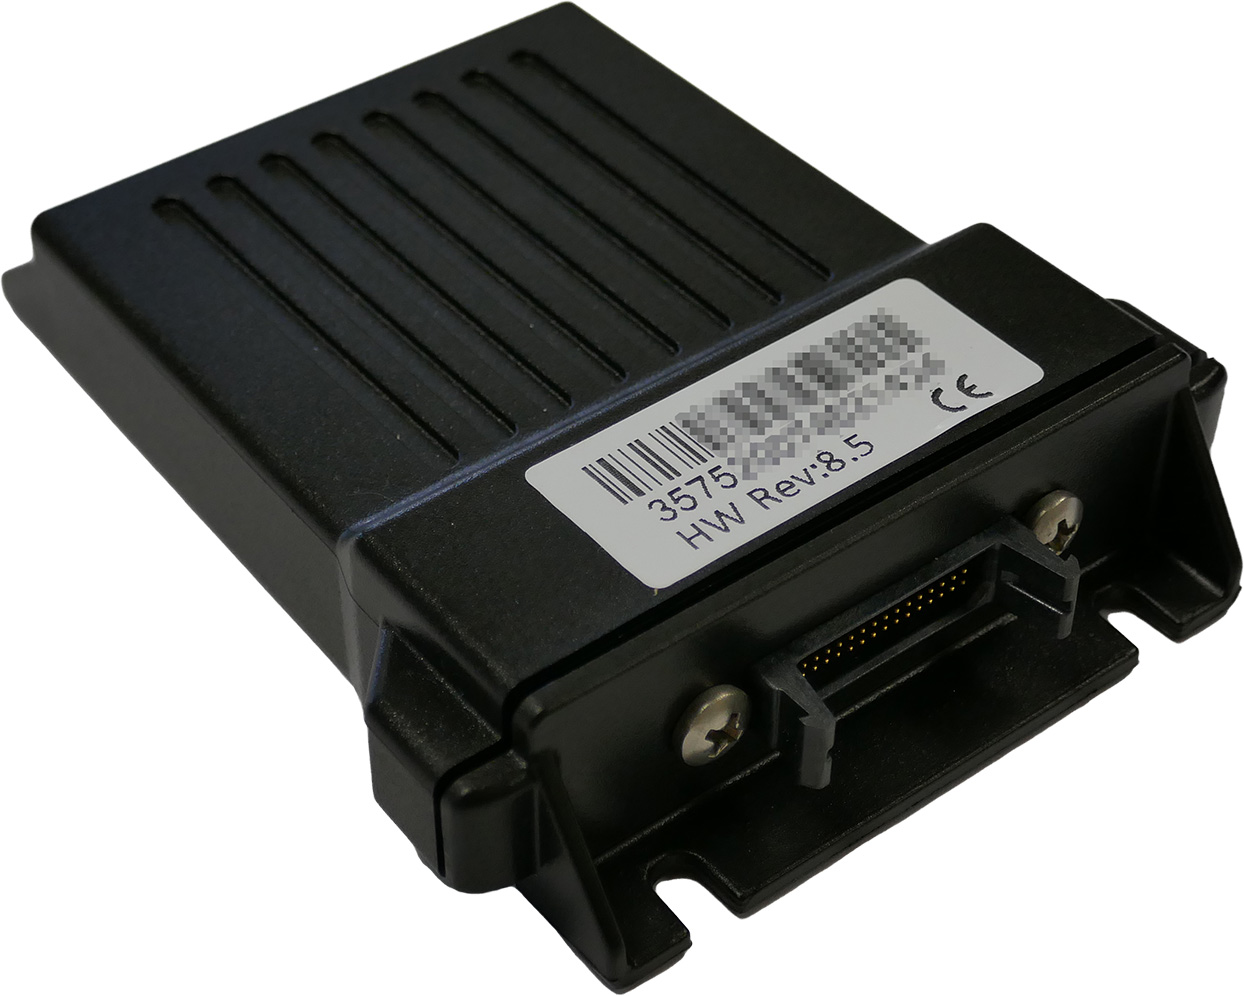
\includegraphics[width=0.4\linewidth]{at240-rs}
	\caption[Astra Telematics AT240 vehicle tracking device]{An Astra Telematics AT240 vehicle tracking device used in our vehicle fleet network.}
	\label{fig:9:vtmodem}
\end{figure}

The AT240 (shown in Fig.~\ref{fig:9:vtmodem}) are capable of vehicle tracking through a Global Navigation Satellite System (GNSS) over the ublox EVA-M8M module~\cite{u-blox_ag_eva-m8_2016}, and are IP67 waterproof rated, making them suitable for our watercraft projects. Each tracking device is based on a Cortex M3 microcontroller~\cite{yiu_armv8-m_2015}, which is powered by a 510 mAh battery that is able to sustain three days of hourly updates, and a three-axis accelerometer to detect motion and driving behaviours. Input/output options include six digital inputs and five digital outputs, as well as two inputs connected to an analogue-to-digital converter. 

\nomenclature[z-gnss]{GNSS}{Global Navigation Satellite System}
\nomenclature[z-can]{CAN}{Controller Area Network}
\nomenclature[z-obd]{OBD}{On-board diagnostics}

The five digital input lines of the tracking devices are connected to the air conditioning, ignition, headlights, radio and, heater statuses. The analogue input line is connected to a battery level logging device that outputs the battery level percentage as an analogue voltage. The battery meter counts the energy flowing in and out of the main electric vehicle battery pack using a current sensor. Serial communications are facilitated through the RS232 standard. In the case of our road vehicles, these connect through OBD-II over a CAN bus, which transmits the vehicle’s journey information to the tracking device. This journey information supplements the sensor readings from the device which are then packaged and transmitted over to our server.

The charging system monitoring is done with a Python daemon running the Threading Socket server library. This library listens for TCP connections on a defined port and creates a new thread for each one, which can handle the processing of the data received. The processing is done by parsing the incoming message from the byte stream into Python variables, connecting to the database and inserting the new data points. Each vehicle connects to our local server via a dedicated port over TCP, where the vehicles are identified through the devices’ IMEI number. The tracking devices transmit telemetry messages to the server using Astra’s proprietary Protocol A. This script connects to the same database and deciphers each incoming packet from the vehicles. 

\nomenclature[z-imei]{IMEI}{International Mobile Equipment Identity}

The tracking devices’ reporting frequency is determined by the vehicle’s ignition state. In other words, a vehicle that is running (positive ignition) will transmit data every minute; whereas a vehicle that is parked (negative ignition) will transmit data every half hour. Charging is facilitated through the vehicle’s 12 V rail, which is connected in line over a 1 A fuse to the vehicle’s battery.

\subsection{Database}
\label{sec:9:vt:db}
Our server’s vehicle tracking daemon receives and parses all incoming telemetry data from the vehicles, which is subsequently appended into the \texttt{telemetry} table in the PostgreSQL database. The following information is recorded in the database for each data point --- latitude, longitude, time logged on device, time received at server, vehicle speed, vehicle heading, altitude, journey max speed, journey max acceleration, journey distance, journey idle time, ignition status, alarm line status (unused), air-conditioning status, headlights status, heater status, charging status, and car battery level The GPS positions and line inputs are uploaded onto the server either at every minute or at every ten meters, whichever comes first.

The server runs a separate parsing script, scheduled as a cron job, to further process and classify the variables into three separate and redundant tables.
\begin{enumerate}
	\item The \texttt{journeys} table records data pertaining to journeys made with the condition that the device records an increase in distance travelled. Entries are appended at one-minute intervals.
	\item The \texttt{charges} table is appended from any telemetry data that whenever the vehicle is charging, are appended at one-minute intervals.
	\item The \texttt{events} table logs and timestamps any appends pertaining to charges and journeys, summarising and batching each data parsing event according to the vehicle’s IMEI number.
\end{enumerate}
This is followed by ten cron-scheduled Python scripts that calculate and update the imported entries for these tables, activating every 30 minutes. These scripts perform the following:
\begin{itemize}
	\item Generate vehicle journeys, charging events, idle events, missing data events.
	\item Generate charging station events.
	\item Combine similar charging station and vehicle charging events based on user tag, time and location.
	\item Compress data, such as air conditioning, heater, headlights into a data point for a journey.
	\item Compress charging data into charging/maintaining charge, divide into by-hour and by-week arrays.
	\item Generate heat maps.
\end{itemize}

As separate scripts are used for different functions, adding new functionality or statistics can be easily done by adding an additional script. This limits the need for modifying existing software and reduces integration problems and helps in isolating errors.

The following paragraphs detail notable information that the data import relates:

\paragraph{Charging places} By assuming that each charging event will take place at either the trial participant’s workplace, home or a public charging station, each participant nominates a work and home location for charging. Charging places are hence classified as charging stations, workplaces and homes with their data stored in a separate table in the database.

\paragraph{Data loss} As each tracking device is programmed to transmit data at every minute when the vehicle is running, and every 30 minutes when the vehicle is parked or idle, any subsequent data packets that arrive later than 30 minutes will be identified as a data loss, these are recorded into a \texttt{data\_loss} table.

\paragraph{Time series modelling} Data from the telemetry table are parsed into day/week time series representation through scripts 8 and 10. This is done by selecting and grouping telemetry data from day and week segments. Travelling distances and energy consumption is summed as they are appended into the \texttt{charges} and \texttt{journeys} tables. Time series modelling is vital for the visualisation of our vehicles’ data as they are disclosed to trial participants to gauge and understand their driving habits.

\subsection{Data Visualisation}
REView visualises vehicle data across four categories --- vehicle tracking, driving statistics, heat maps and journey logs, as detailed in their subsections. All visualisations are presented on REView’s front end, which is presented through a PHP script that connects to any of the three related tables on the database through SQL queries. Users wanting to view their vehicle’s data on REView are required to log in with their credentials, which is linked to their registered vehicles. In this context, we establish a one-to-many relationship between the User and Cars tables in the database. We use a one-month sampling period to represent the figures in this section.

\subsubsection{Vehicle Tracking}
The vehicle tracking page looks up a list of vehicles that corresponds to the user viewing it. The user can select an individual vehicle or all vehicles in a fleet and the time period to display. The graph is interactive, allowing the user to drag and zoom in on the time scale. 

This page uses PHP scripts to supply the information to JavaScript code on the page using several free-to-use libraries including JQuery~\cite{noauthor_jquery_2019} for communication with the server, Google Maps for the map and Dygraph~\cite{vanderkam_interactive_2019} for the interactive graph. The Dygraph library is open source and was modified for use in the website. 

To display the GPS data, the map has the ability to show individual interactive points that can be clicked on for additional information or an image that is generated by a PHP script on the server. The number of interactive points is limited to 150, as too many points can cause instability in the browser. However, the image overlaid over the map can contain any number of points, which allows users to see data over longer time periods. Generating an image at the server is also useful, because the information sent from the server to the user is significantly less. The server caches all images generated and generates differently scaled images for different map zoom levels.

For performance and stability reasons, the graph below the map is limited to displaying 2,000 points at a time. To reduce the load on the server, the graph caches data and only requests additional information when necessary. When a user pans the graph to the left or right, only the missing information is requested. The granularity of the data is also important, and the server is designed to send sub-divided data when the time period selected has more than the 2,000-point maximum. When the user zooms on a section of the graph, the server is asked for sub-divided or raw information for this smaller time period. 

A query reads all IMEIs associated to that user and retrieves a list of related vehicles from the Cars table, which is subsequently presented as a selectable radio button list. For each selected vehicle, the vehicle tracking page visualises the vehicle’s position and its trajectory from the selected time period, which is displayed using the Google Maps JavaScript API. The vehicle’s current location is given as a colour-coded pin that corresponds to the selected vehicle, whereas its trajectory is plotted through an array of markers obtained from the vehicle’s historical location data from the telemetry table. 

Additionally, the vehicle tracking page also includes a chart that allows users to check, by defining a sampling period, the vehicle’s driving behaviour as a time series, which is also exportable as a \textit{*.csv} file. REView plots multiple line graphs on this chart, which includes battery levels, vehicle speed, travelled distance, as well as air conditioning, headlights and heater usage. Fig.~\ref{fig:9:vt:vis:vt} shows an example of this visualisation.

\begin{figure}[H]
	\centering
	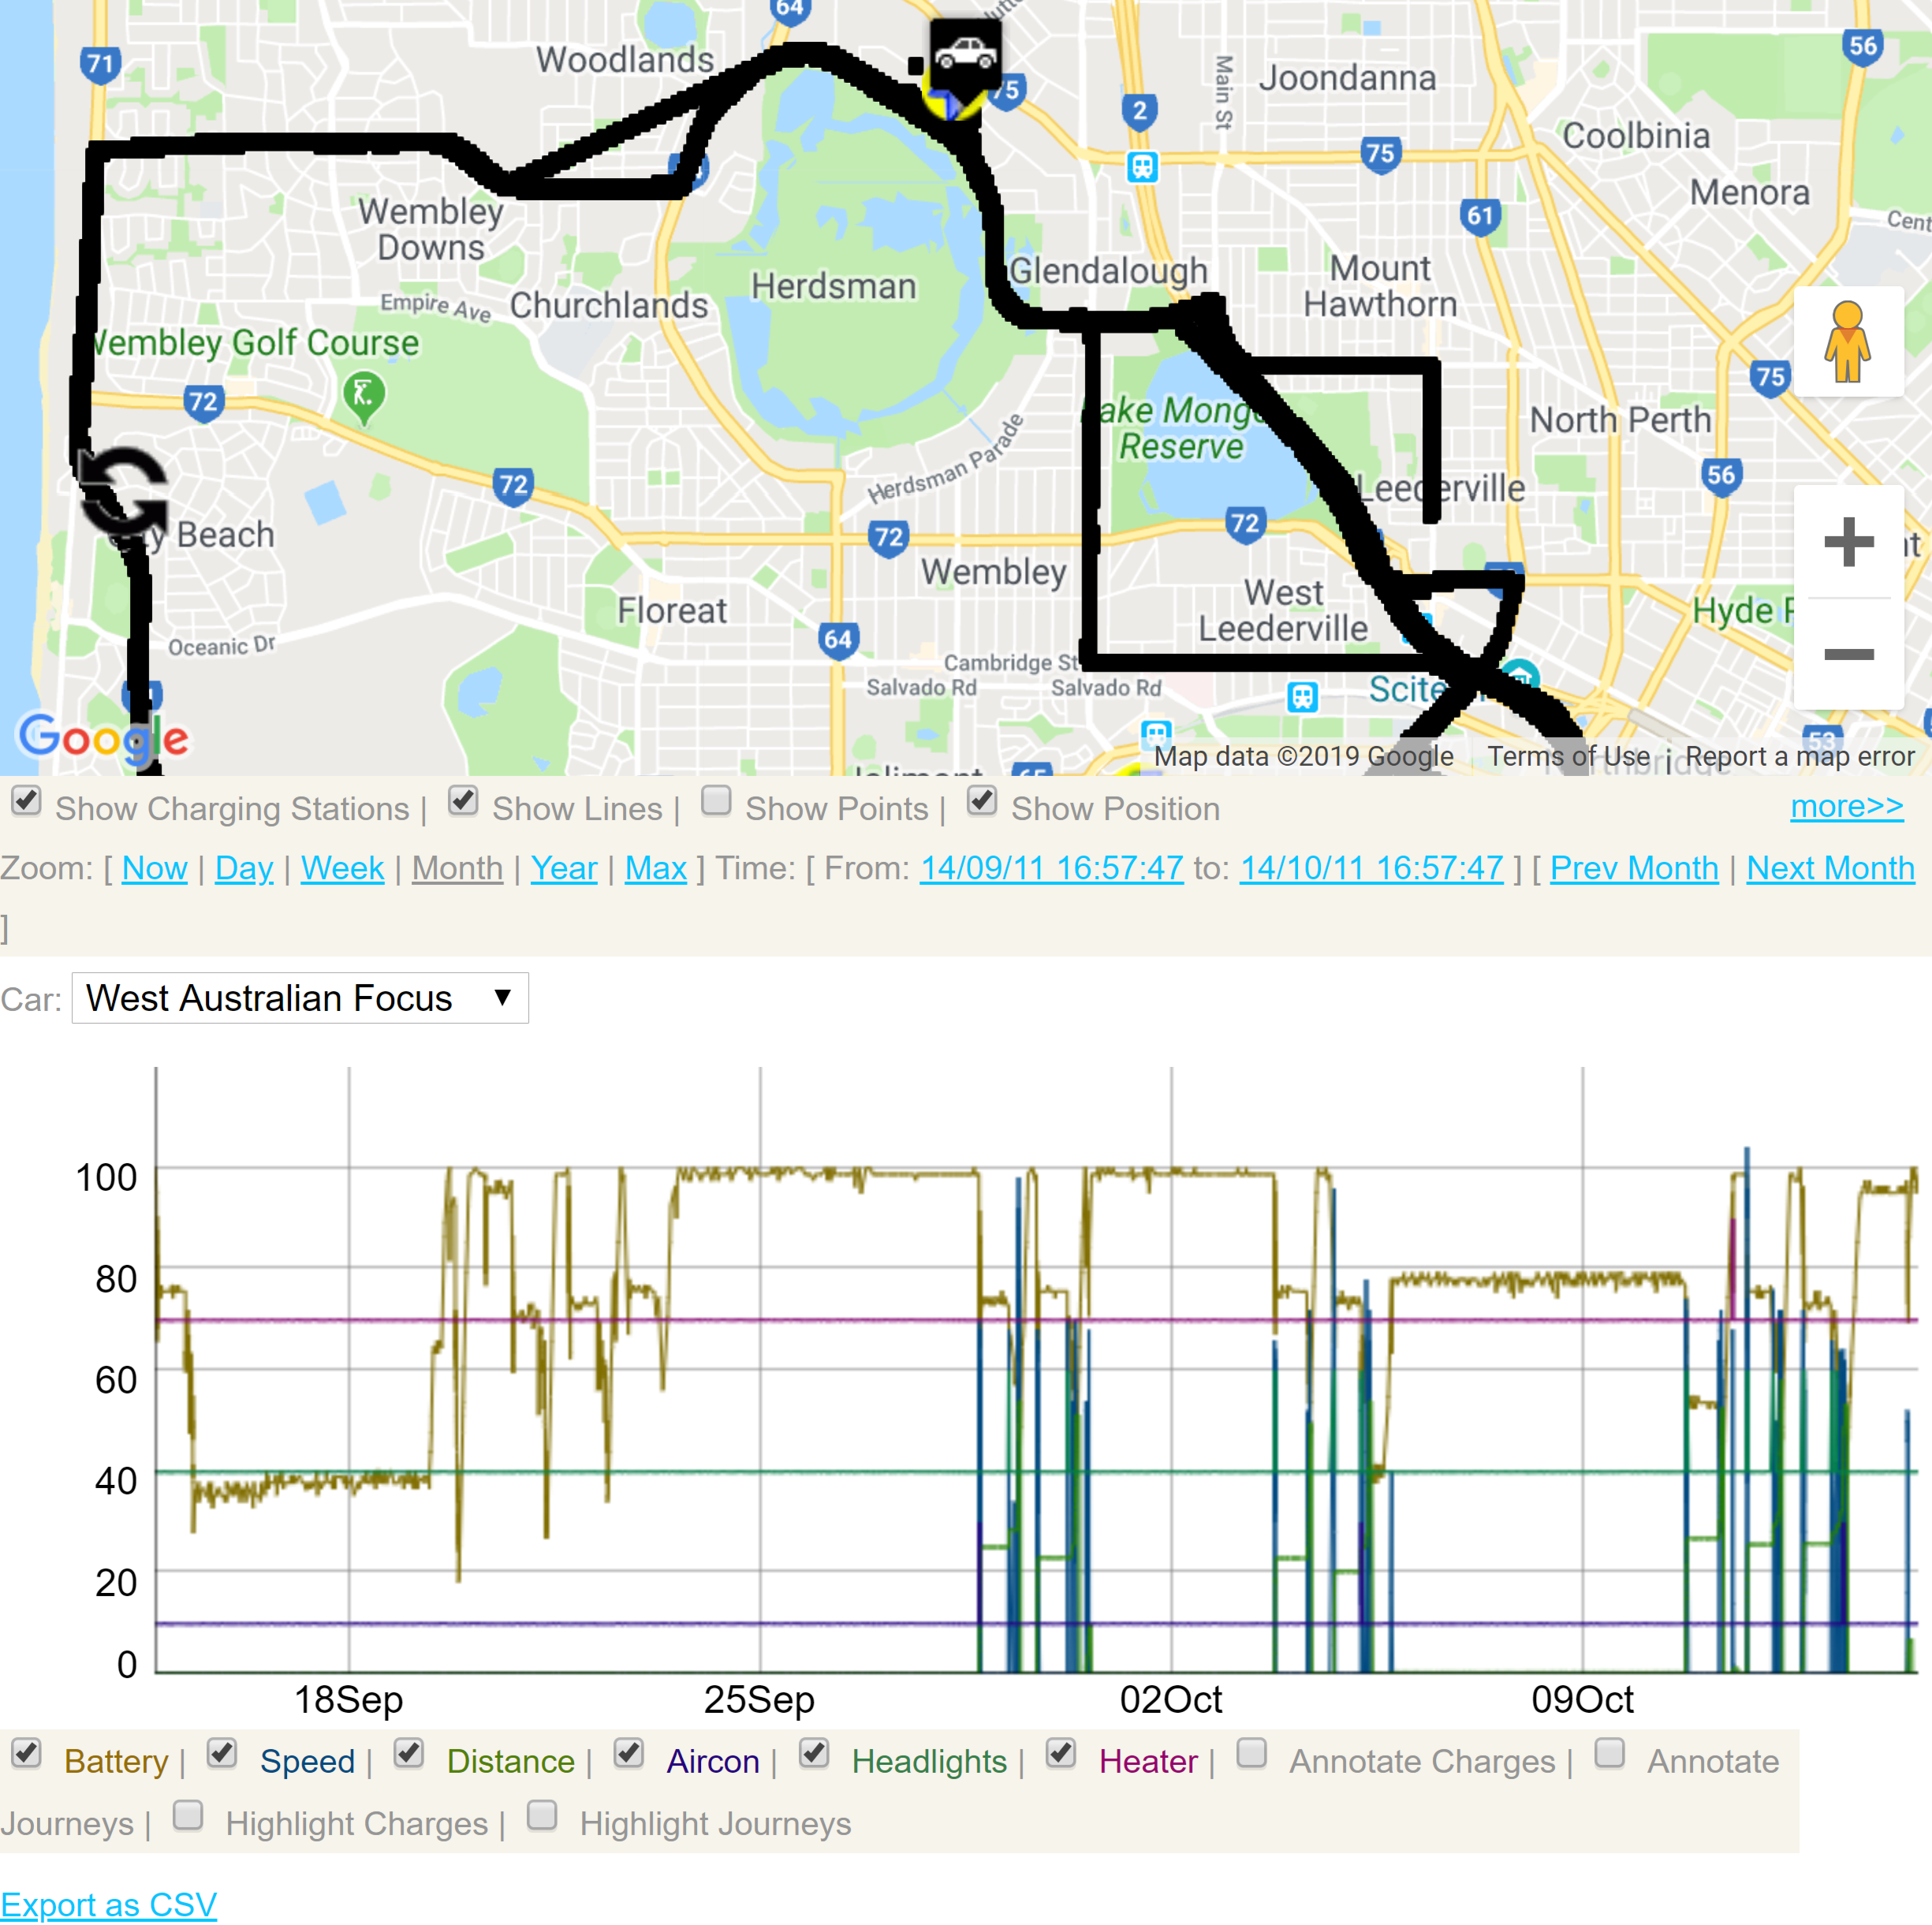
\includegraphics[width=0.9\linewidth]{vt-t-vis-vt}
	\caption[Vehicle tracking page screen grab]{Partial screen grab of the vehicle tracking page showing its historical trajectories on Google Maps, and its driving behaviours in the bottom chart.}
	\label{fig:9:vt:vis:vt}
\end{figure}

\subsubsection{Driving Statistics}
Visualisation for driving stations is presented in two modes --- one as an overview for all vehicles, and another for a detailed analysis of driving patterns. The overview page consolidates statistics across all vehicles, and for a specific range of dates, with examples as shown in Fig.~\ref{fig:9:vt-t-vis-ds1}.

\begin{figure}[H]
	\centering
	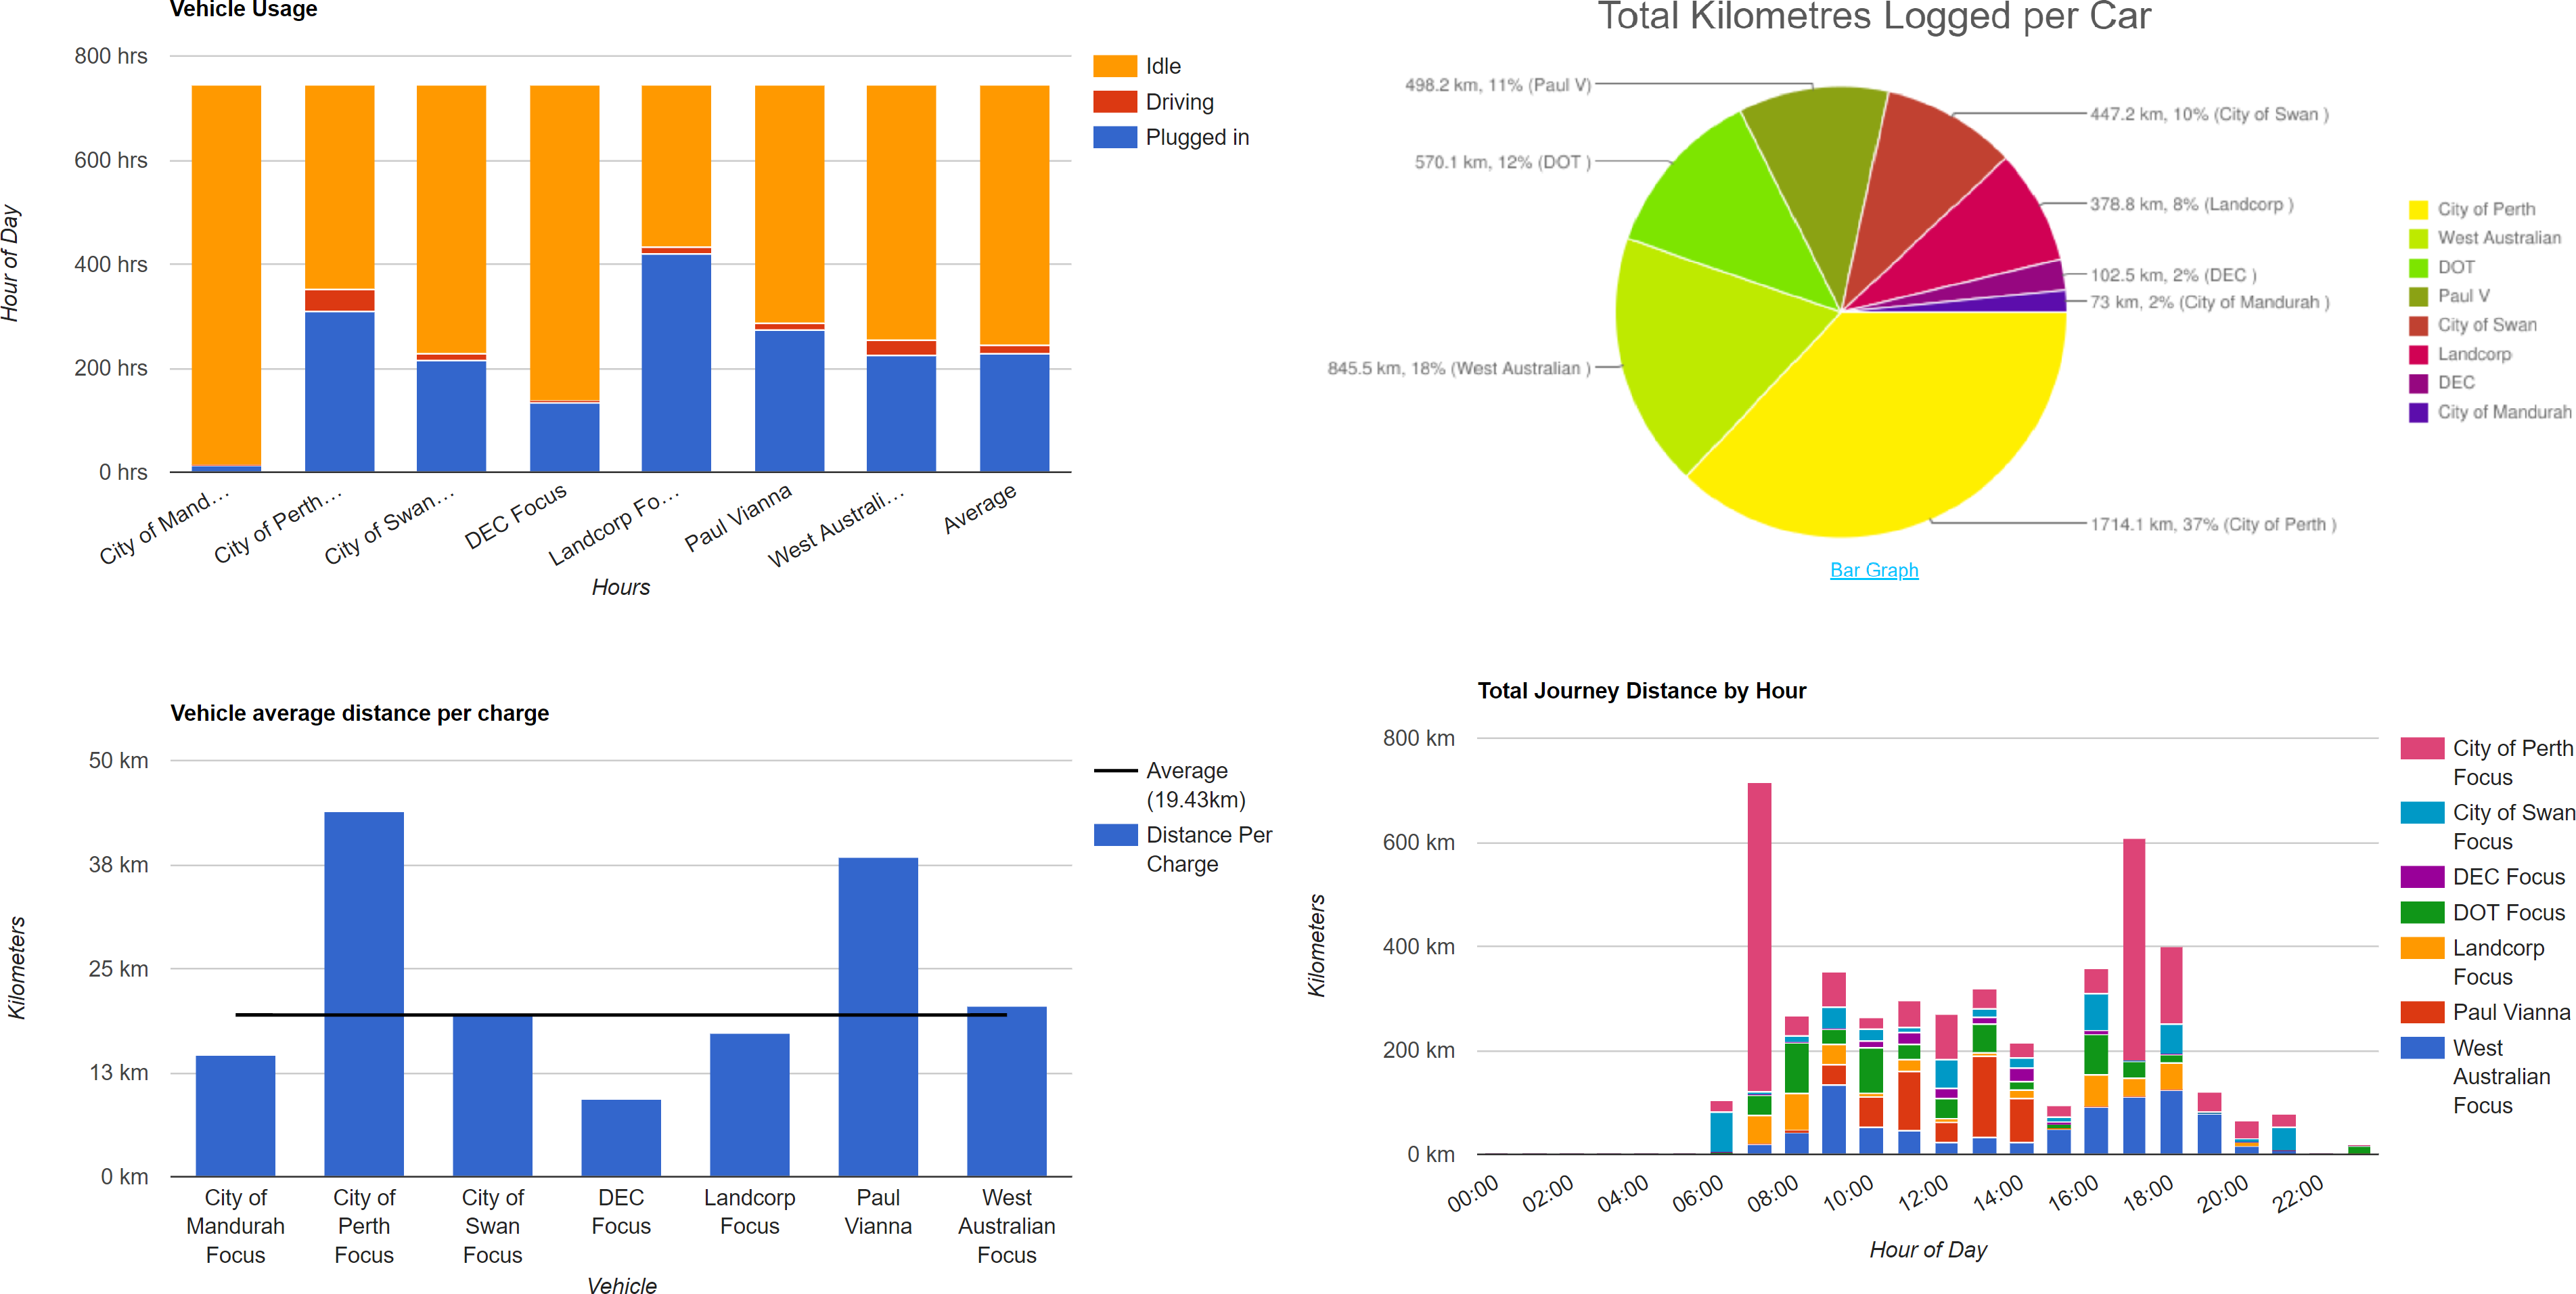
\includegraphics[width=\linewidth]{vt-t-vis-ds1-crop}
	\caption{Examples of charts showing driving data.}
	\label{fig:9:vt-t-vis-ds1}
\end{figure}

\paragraph{Leaderboard} The leaderboard table ranks the vehicles according to their distance travelled and compares them alongside the other vehicles. The table also lists the vehicles’ driving times, total number of journeys, average journey distance and average journey time. An example of the leaderboard is shown in Fig.~\ref{fig:9:vt-leaderboard}.

\begin{figure}[H]
	\centering
	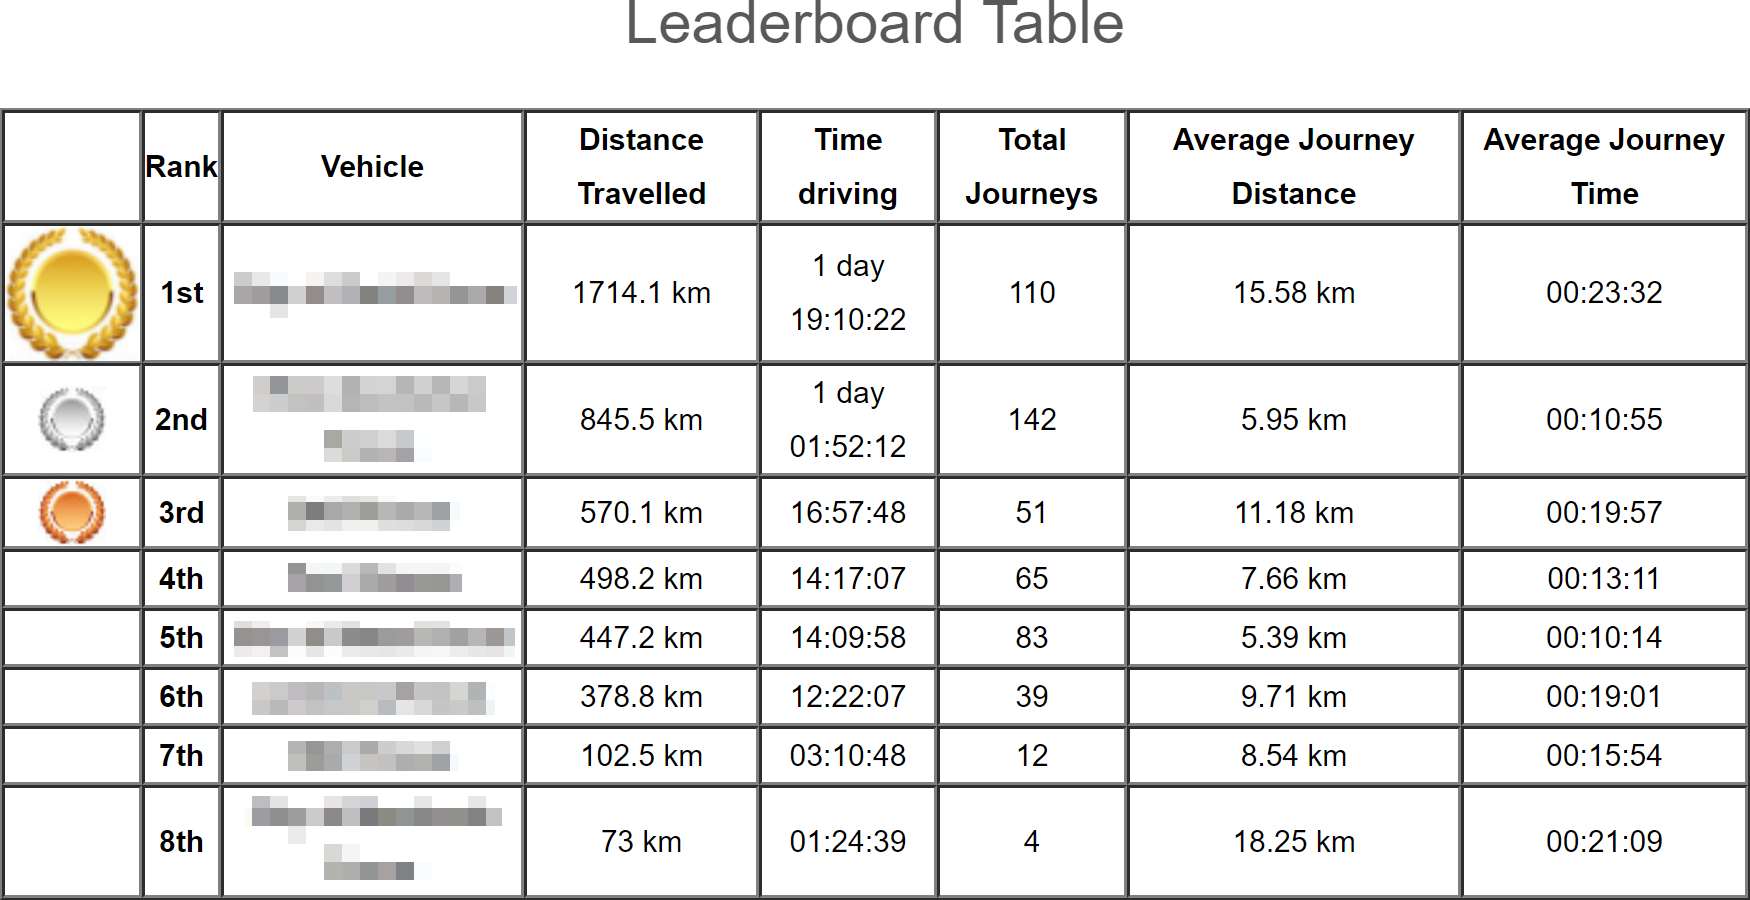
\includegraphics[width=\linewidth]{vt-leaderboard-crop}
	\caption[Sample leaderboard displaying driving statistics for the trial vehicles]{A sample leaderboard displaying driving statistics for the trial vehicles for an average month. Vehicle names have been pixelated to preserve privacy.}
	\label{fig:9:vt-leaderboard}
\end{figure}

\paragraph{Chart legends} Legends used in the charts are described according to their:
\begin{itemize}
	\item Vehicle name: Name of vehicle e.g. UWA Lotus, UWA Getz etc.
	\item Location type: Type of charging station location e.g. home, business or public station.
	\item Vehicle state: Vehicle status e.g. idle, driving or plugged in.
	\item Plug type: Charging current e.g. 32 A, 15 A or 10 A.
	\item Daily distance travelled in km, with an average plot.
\end{itemize}

Likewise, driving statistics for the individual vehicles are presented across three sections --- distance, charging and journeys, as shown in Fig.~\ref{fig:9:vt-t-vis-ds2}. For each statistic, results from each vehicle are compared against the average results from the rest of the vehicles (community). This, along with the leaderboard, is a gamification feature, which we find useful to keep monthly reports interesting for the users. These are mostly presented in bar charts of grouped pairs to illustrate the statistical difference between that vehicle and the community.

\begin{figure}[H]
	\centering
	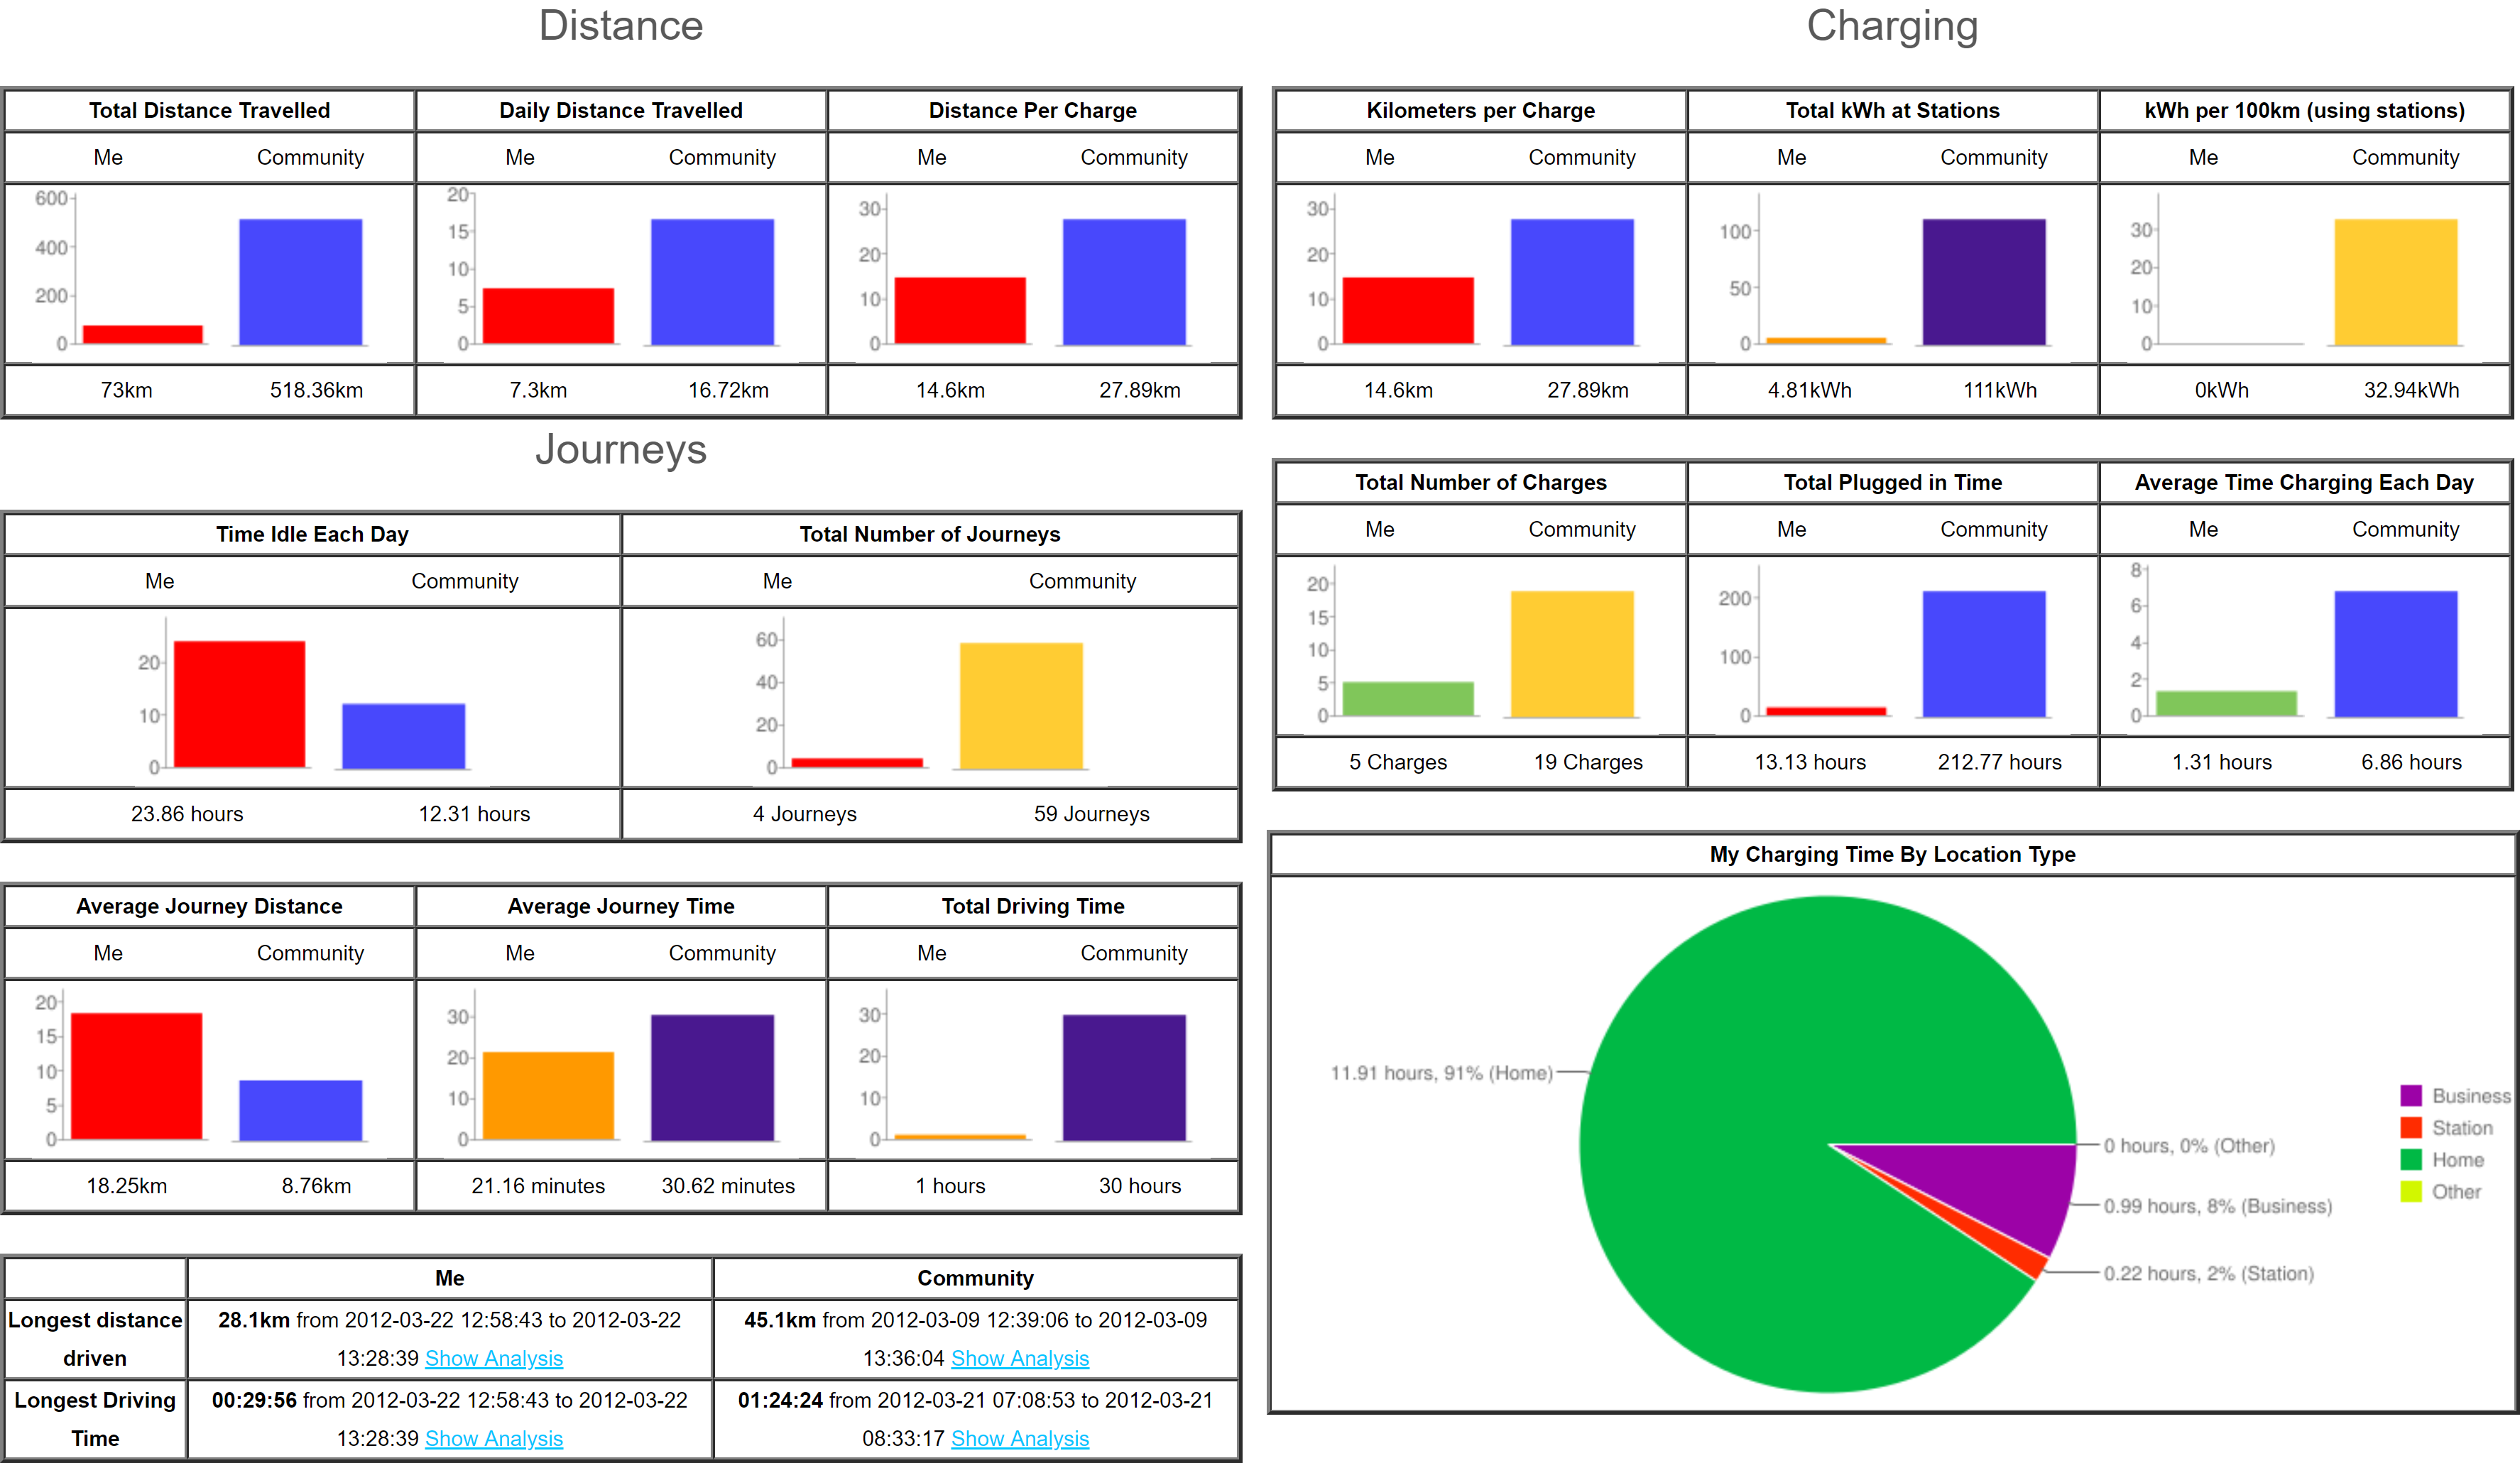
\includegraphics[width=\linewidth]{vt-t-vis-ds2}
	\caption[Individual driving statistics]{Individual driving statistics are presented in distance, journeys and charging sections.}
	\label{fig:9:vt-t-vis-ds2}
\end{figure}

\subsubsection{Heat Maps}
REView generates heat maps of the tracked vehicles through the aggregation of their GPS coordinates and location type geofencing. They are automatically generated and can show areas where vehicles drive, park and charge within certain time periods. The server periodically runs a heat map generating Python script as a cron job, which searches through the journeys, charges, telemetry and any low charges from the journeys table, eventually generating a \textit{*.kml} file that contains the location of the heat maps.

The Python script imports Jeffrey Guy’s heatmap library~\cite{guy_python_2019}, which utilises the Python Imaging Library (PIL) to generate a heat map \textit{*.kml} file along with a \textit{*.png} file containing an image overlay that corresponds to the heat maps. Areas with increasing overlapping entries from the database will progress from a navy to a red hue, as shown in Fig.~\ref{fig:9:vt-t-vis-hm}. These heat maps can be generated according to the user’s selection, which includes the type of heat map (places parked, charged or driven), time frame (year or month) and time period.

\nomenclature[z-pil]{PIL}{Python Imaging Library}

\begin{figure}[H]
	\centering
	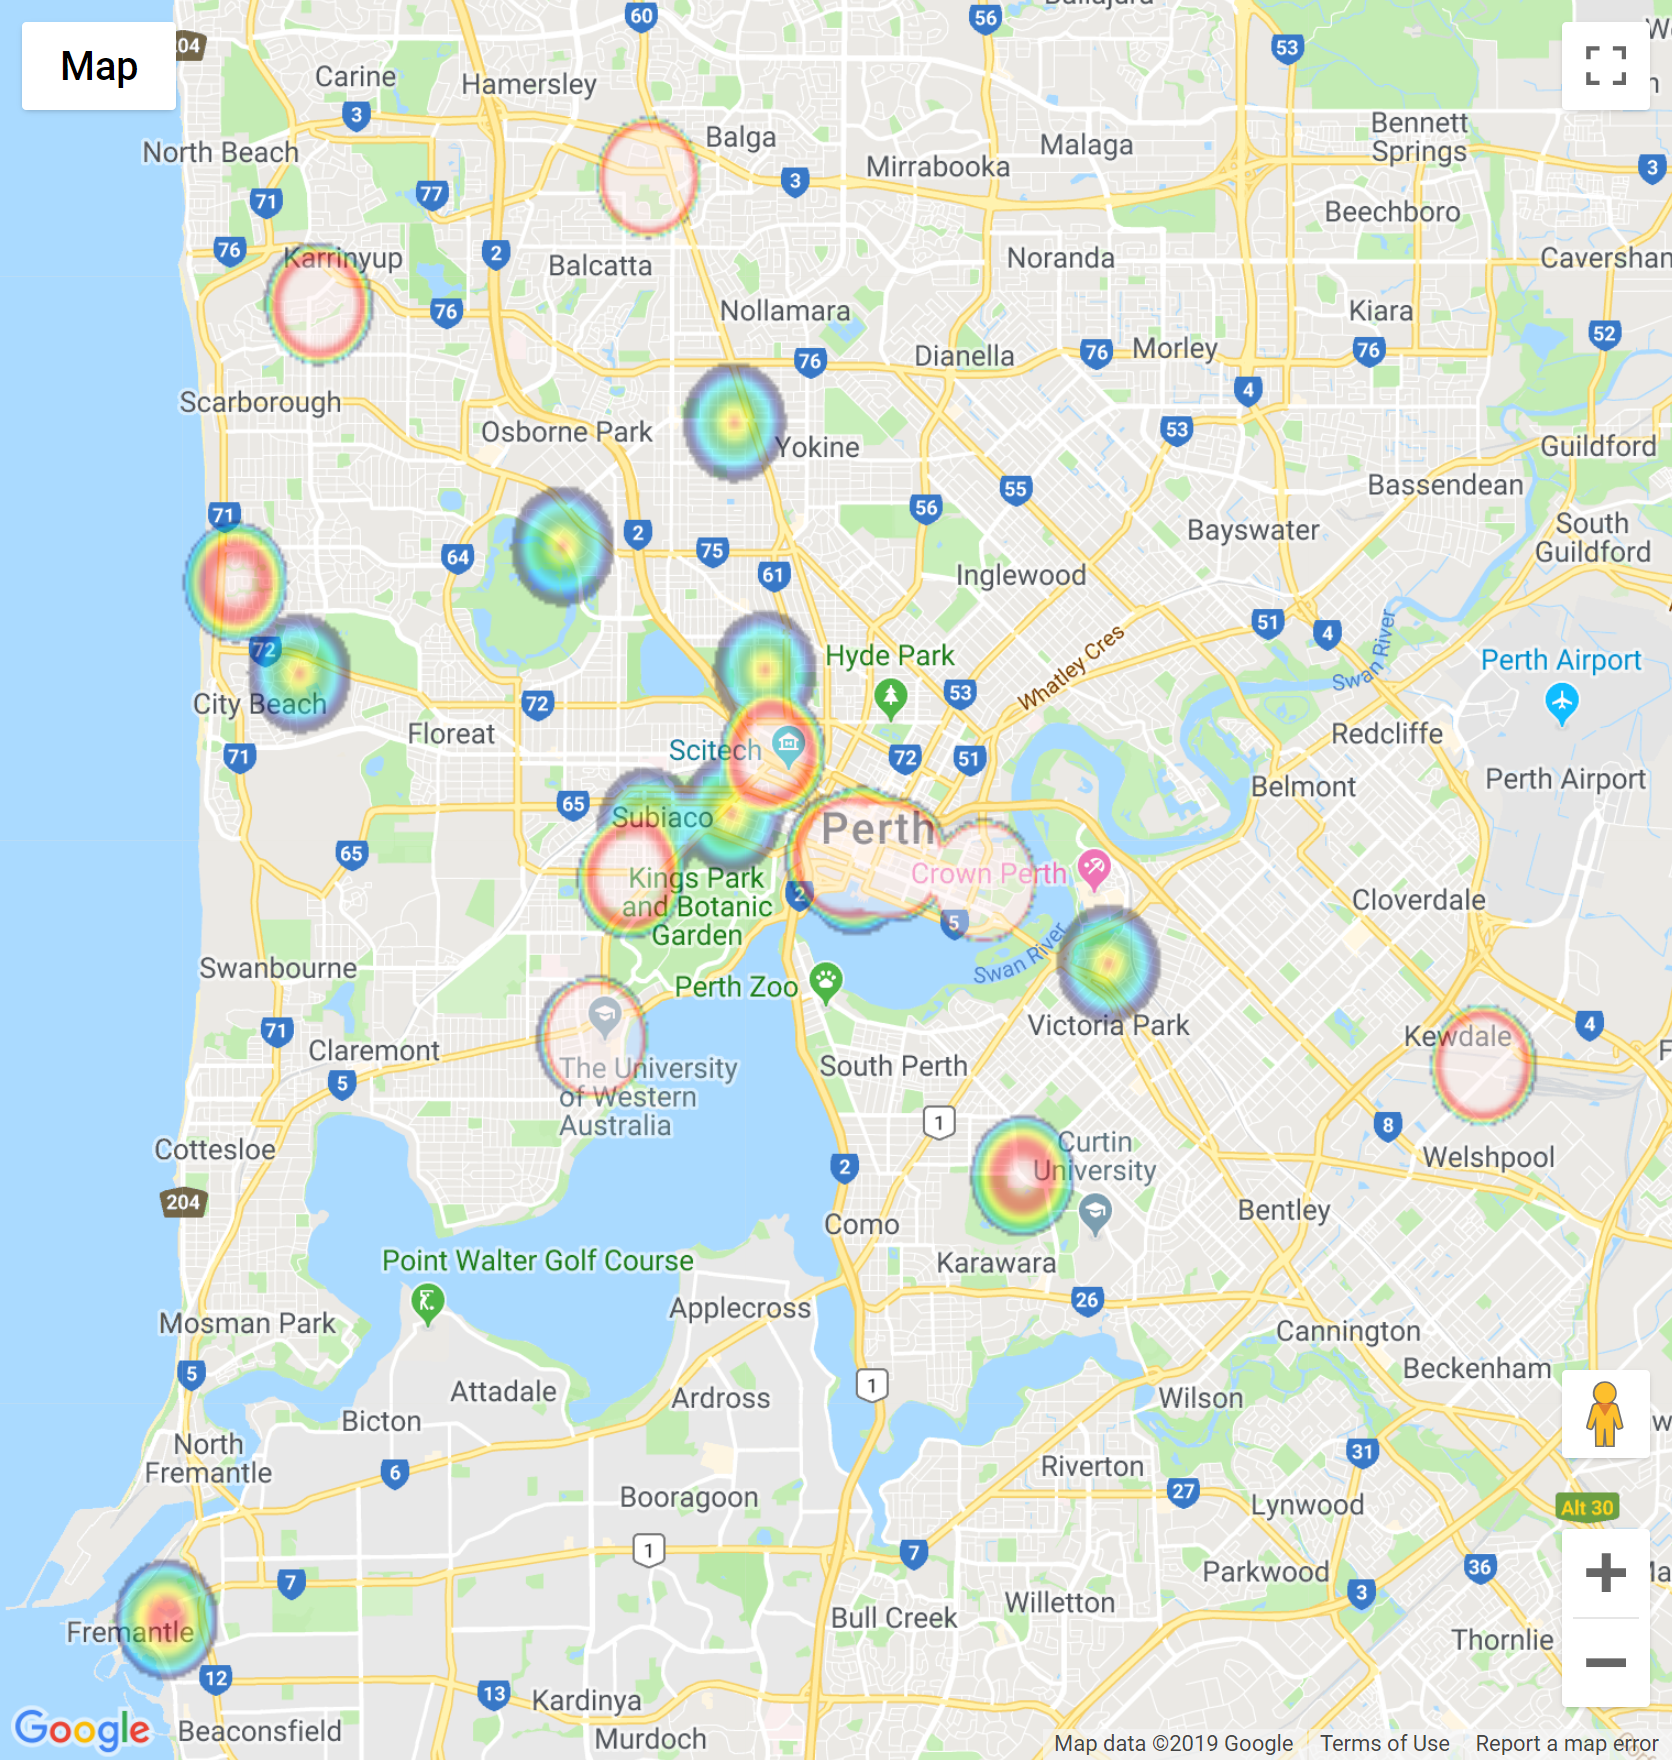
\includegraphics[width=0.8\linewidth]{vt-t-vis-hm}
	\caption[Heat map of the vehicle fleet tracked over a month]{Heat map of the vehicle fleet tracked over a month for possible charging locations that are utilised during the day (7 am to 6 pm).}
	\label{fig:9:vt-t-vis-hm}
\end{figure}

\subsubsection{Journey Logs}
The completion of any drive routine from a tracked vehicle will result in the tabulation and display of its journey log onto REView as shown in Fig.~\ref{fig:9:vt-t-vis-j}.

The cost of equivalent petrol, electricity and carbon emissions are calculated based on the distance travelled, which is 10.43 cents, 3.47 cents and 168 g per kilometers respectively. These values were taken off the Carbon Dioxide Emissions from New Australian Vehicles 2013 information paper~\cite{national_transport_commission_carbon_2014} by the Australian National Transport Commission along with current electricity tariffs as an average. The monetary savings are calculated as a difference between petrol and electricity cost. Importing options for \textit{*.csv} data is also available.

\begin{figure}[H]
	\centering
	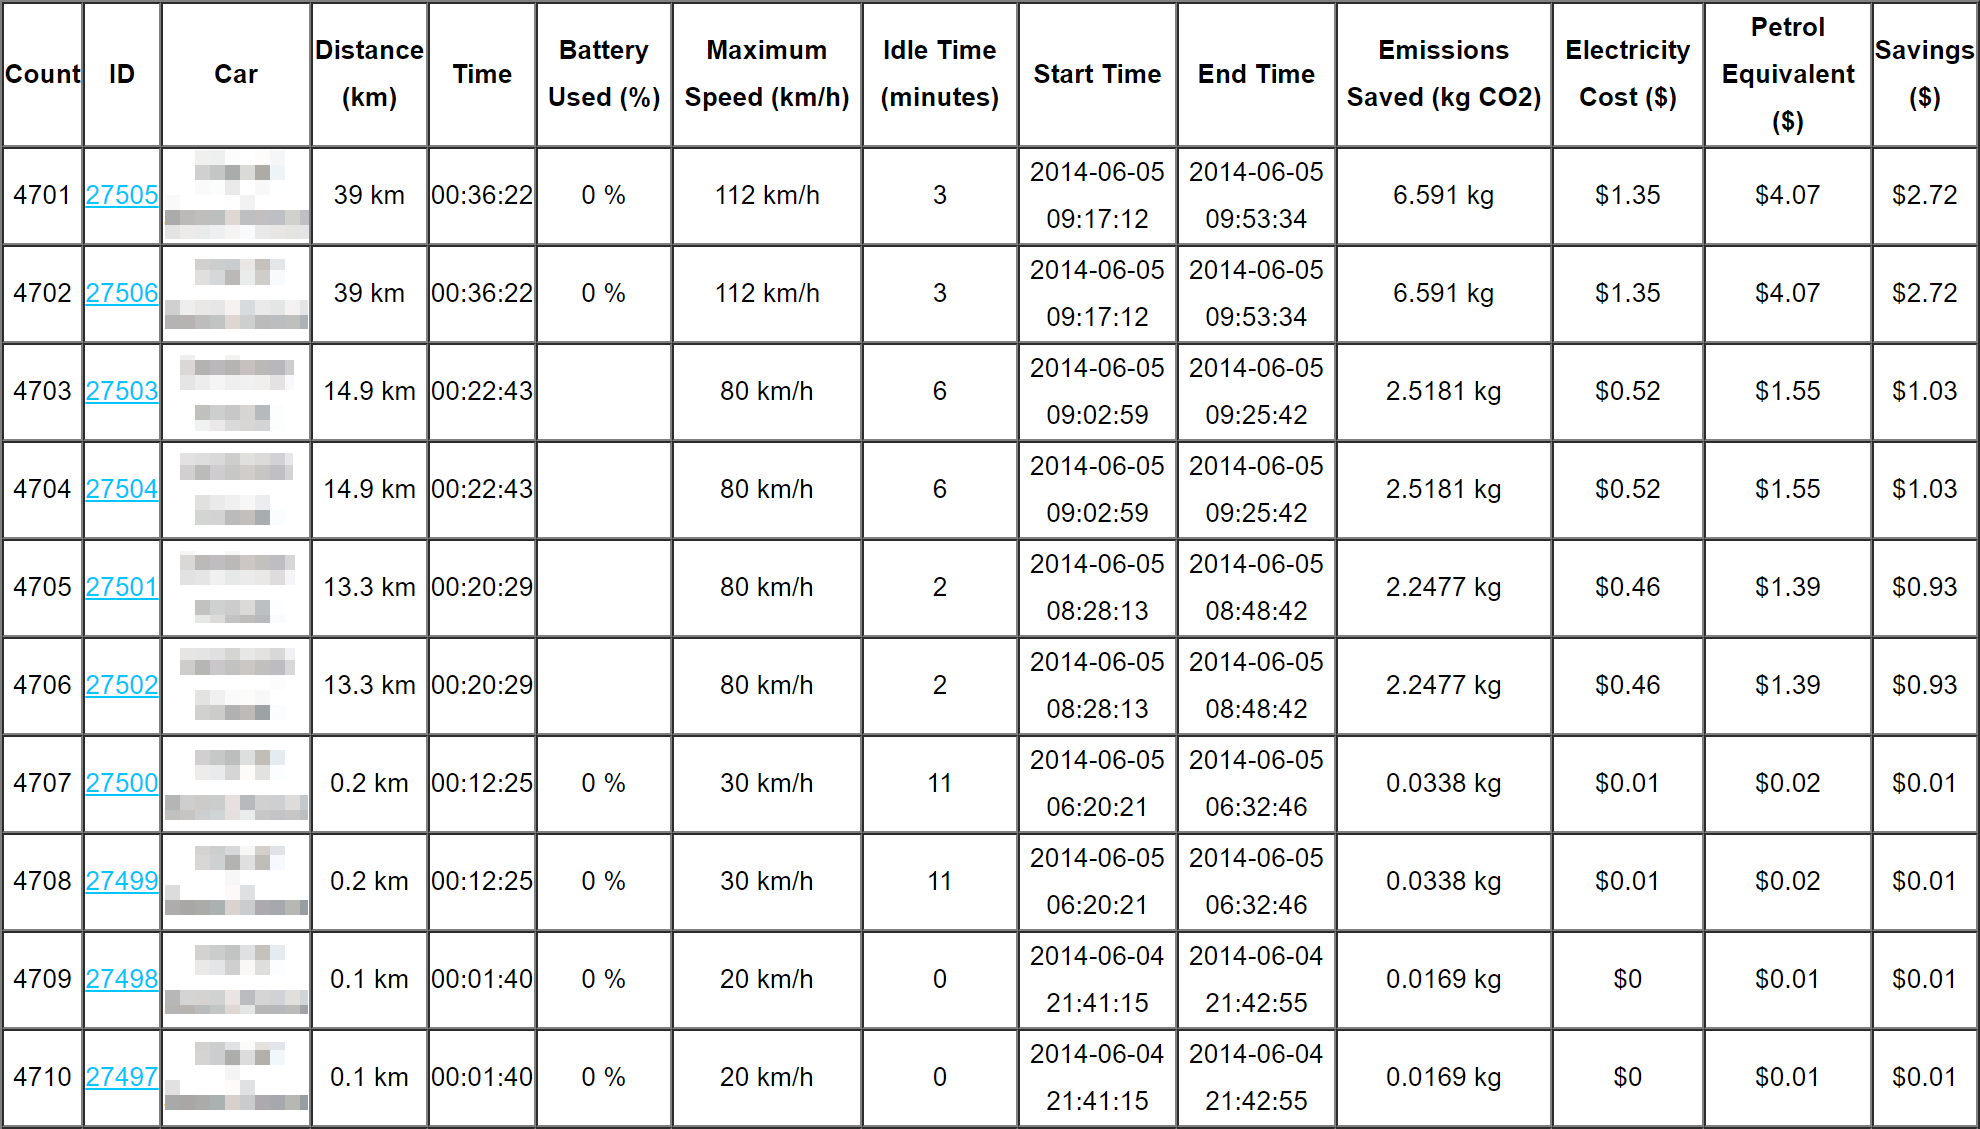
\includegraphics[width=\linewidth]{vt-t-vis-j-crop}
	\caption[Journey logs of a tracked vehicle]{Table showing the journey logs of a tracked vehicle. Vehicle names have been pixelated to preserve privacy.}
	\label{fig:9:vt-t-vis-j}
\end{figure}

\section{EV Charging Power Generation}
\label{sec:9:evpg}
UWA's AC chargers are powered through a solar PV array installed on the roof of the Human Movement building. This is a dual inverter PV plant that is rated at 20 kWp and collectively generates 114.1 kWh per day, which is greater than the combined usage of all our AC chargers. This plant uses two Sunny STP 10000TL-10~\cite{sma_solar_technology_ag_sunny_2017} 10 kW three-phase inverters with a maximum efficiency of 98.1\% at a nominal 600 V. Monitoring on the solar plant is done through SMA's Sunny WebBox~\cite{sma_solar_technology_ag_sunny_nodate}, which provides a web interface for configuration, including that for telemetry data transmission to our local server at up to one-minute intervals. The average instantaneous measurement of the plant is tabulated in Table~\ref{tbl:9:pg}. REView processes data from this infrastructure according to the class diagram in Fig.~\ref{fig:9:uml-pg}.

\begin{table}[H]
	\centering
	\caption{The average instantaneous measurements of the solar PV plant}
	\label{tbl:9:pg}
	\begin{tabular}{ll}
		\toprule
		DC Current        & 1 A                  \\
		DC Voltage        & 510 V                \\
		DC Power          & 1000 W (2 inverters) \\
		AC Grid Frequency & 50 Hz                \\
		AC Grid Power     & 1600 W               \\
		AC Phase Current  & 1.1 A                \\
		AC Phase Voltage  & 225 V                \\
		AC Phase Power    & 500 W                \\
		AC Day Yield      & 56.67 kWh            \\ \bottomrule
	\end{tabular}
\end{table}

\begin{figure}[H]
	\centering
	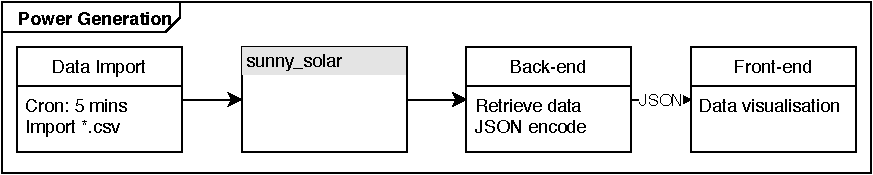
\includegraphics[width=\linewidth]{uml-pg}
	\caption{Simplified class diagram showing REView’s energy generation system.}
	\label{fig:9:uml-pg}
\end{figure}

\subsection{Data Visualisation}
Data from the Sunny WebBox is pushed daily to our server via FTP as a series of \textit{*.csv} spreadsheets, containing timestamped entries at five-minute intervals that record each inverter's instantaneous measurements, similar to Table~\ref{tbl:9:pg}. We subsequently wrote a Python script that imports this data into our server's PostgreSQL database as the \texttt{sunny\_solar} table, which runs on a five-minute cron schedule. This script reads the last event in the table and imports every successive data from the spreadsheet, synchronising the data between the two entities. The data from the solar system includes time stamps, power generated, voltages at the panels and grid and operation health flags. PV systems are connected to and scanned every 15 minutes for data download.

\nomenclature[z-ftp]{FTP}{File Transfer Protocol}

This data in the \texttt{sunny\_solar} table is, in turn, visualised as a series of line graphs on REView's front end, which can be selected through a day, week or month period. Visualisations are given in the solar plant's power and energy generation and consumption, as accumulated from the selected period. We achieve this visualisation by importing the JpGraph~\cite{asial_corporation_jpgraph_nodate} library, whereby a back-end PHP script calls all related SQL queries which then encodes it as a JSON representation for the front end, as Fig.~\ref{fig:9:solar} illustrates.

\begin{figure}[H]
	\centering
	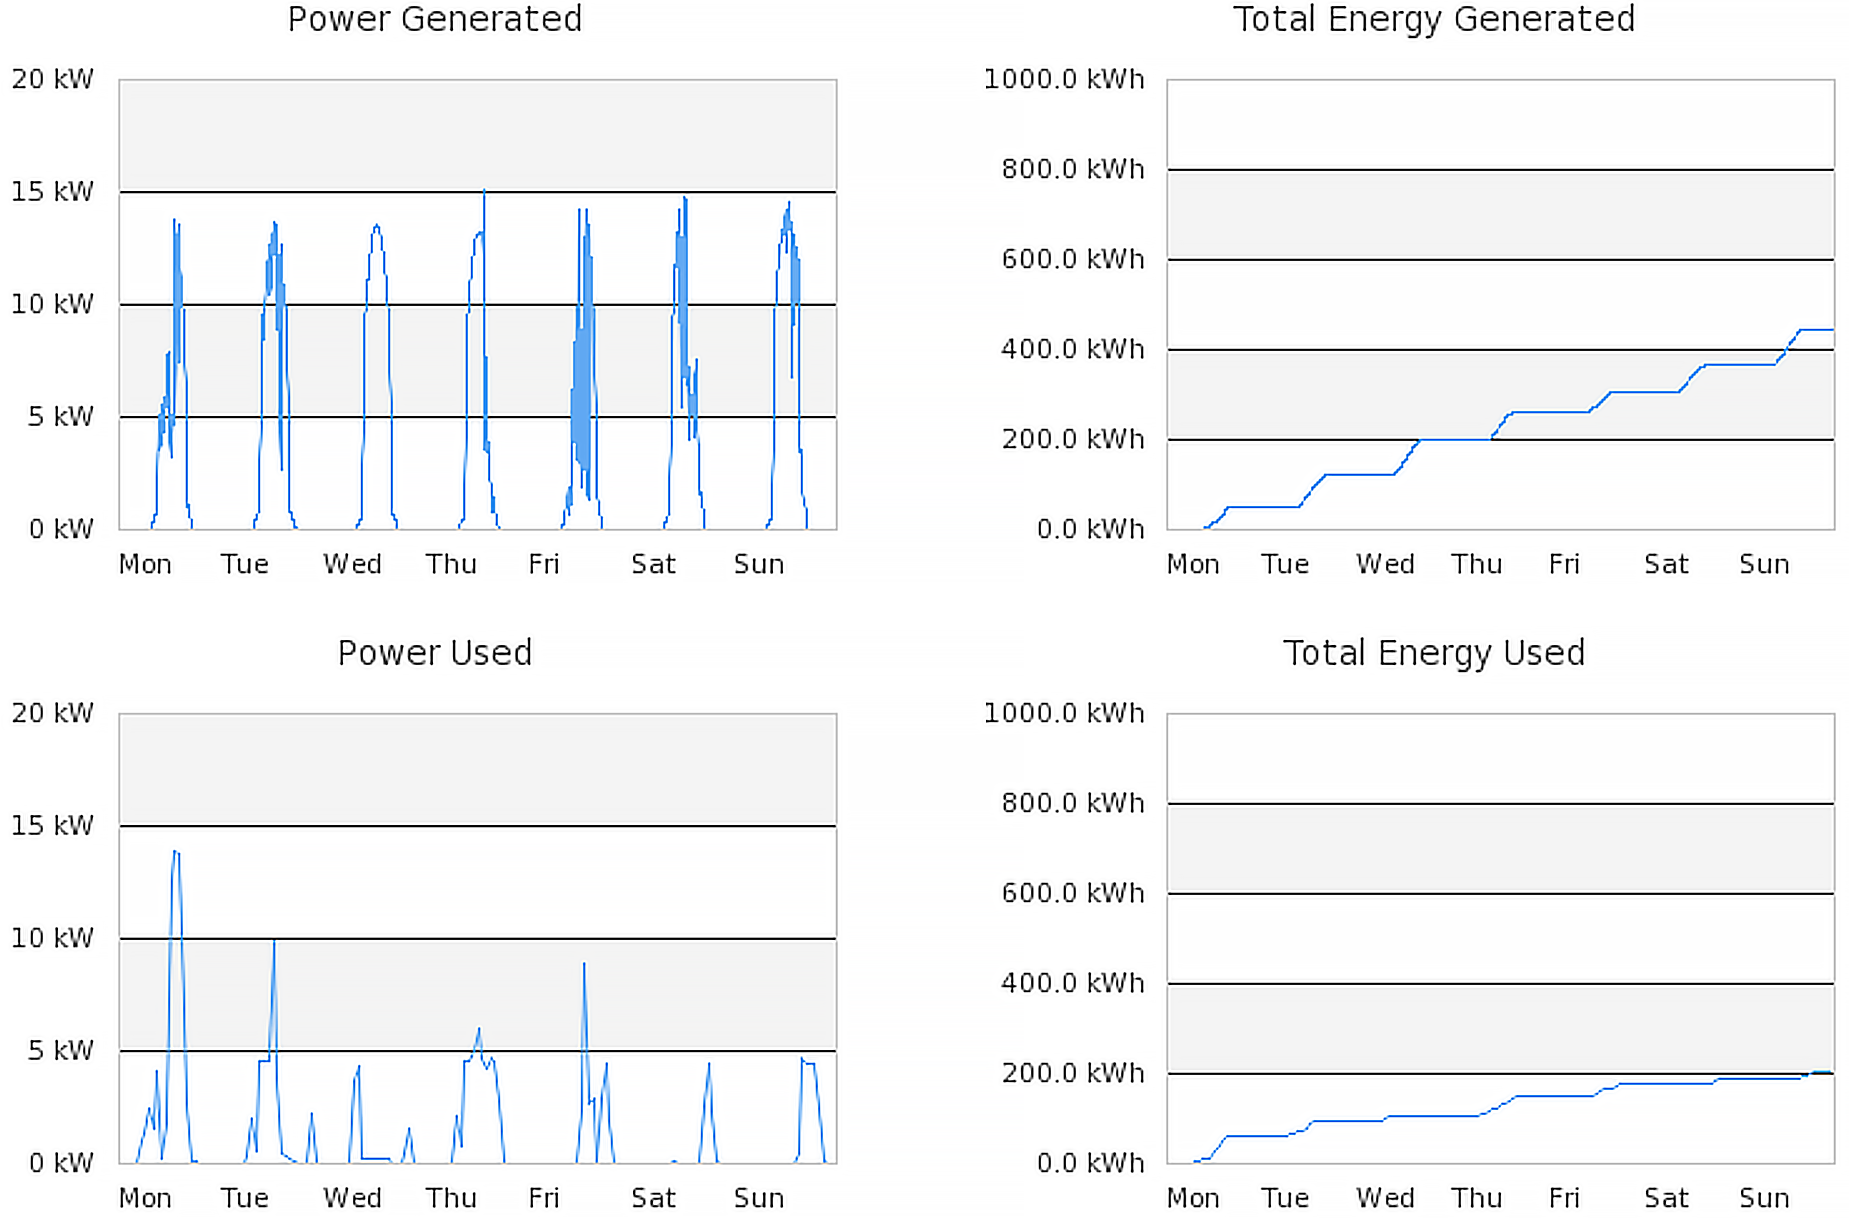
\includegraphics[width=\linewidth]{solar}
	\caption{Graphs generated from solar PV data over a typical week.}
	\label{fig:9:solar}
\end{figure}

\section{Usage Billing}
\label{sec:9:ub}
The billing page allows an EV user to view his or her monthly mobility cost. It also lets station operators view utilisation and energy usage of their stations. In both cases summaries as well as itemised bills are generated. All bills are automatically generated with several informative graphs, including distance travelled, distance per charge and kWh per km of the individual versus the community. Also, a time-of-use energy graph is generated.

To provide users and charging station owners with a summarised update, bills are generated at every first Monday of the month through a scheduled cron job, which is then emailed to related users who opt into this service, where they are classified as either vehicle owners or station operators. For this purpose, we have configured a CSS script that enables the printing of the contents directly through HTML as a Tax Invoice. This is presented as a combination of charts and tables that are dependent on the type of bill presented --- Vehicle/User (User Billing), Charging Station (Station Operator Billing) or Summary (Network Overview). Each bill type is generated through individual PHP back ends that encode SQL queries as a JSON representation as detailed in the subsections.

\subsection{User Billing}
An itemised bill enables users to individually monitor and track their charging behaviours, which is displayed as a line graph followed by three tables (see Fig.~\ref{fig:9:uib}). If the vehicle is part of our tracked fleet in Section~\ref{sec:9:vm}, its driving statistics (total distance travelled, distance per charge and kWh per km) will be presented above the line graph and compared against the rest of the community. REView obtains these data by running a query for each graph or table for a given bill. This query is applied for the \texttt{station\_charges} table according to the accessing user and its selected sampling timeframe, which returns the charging timestamps, duration, location and per-hour energy usage to the front end.

\begin{figure}[H]
	\centering
	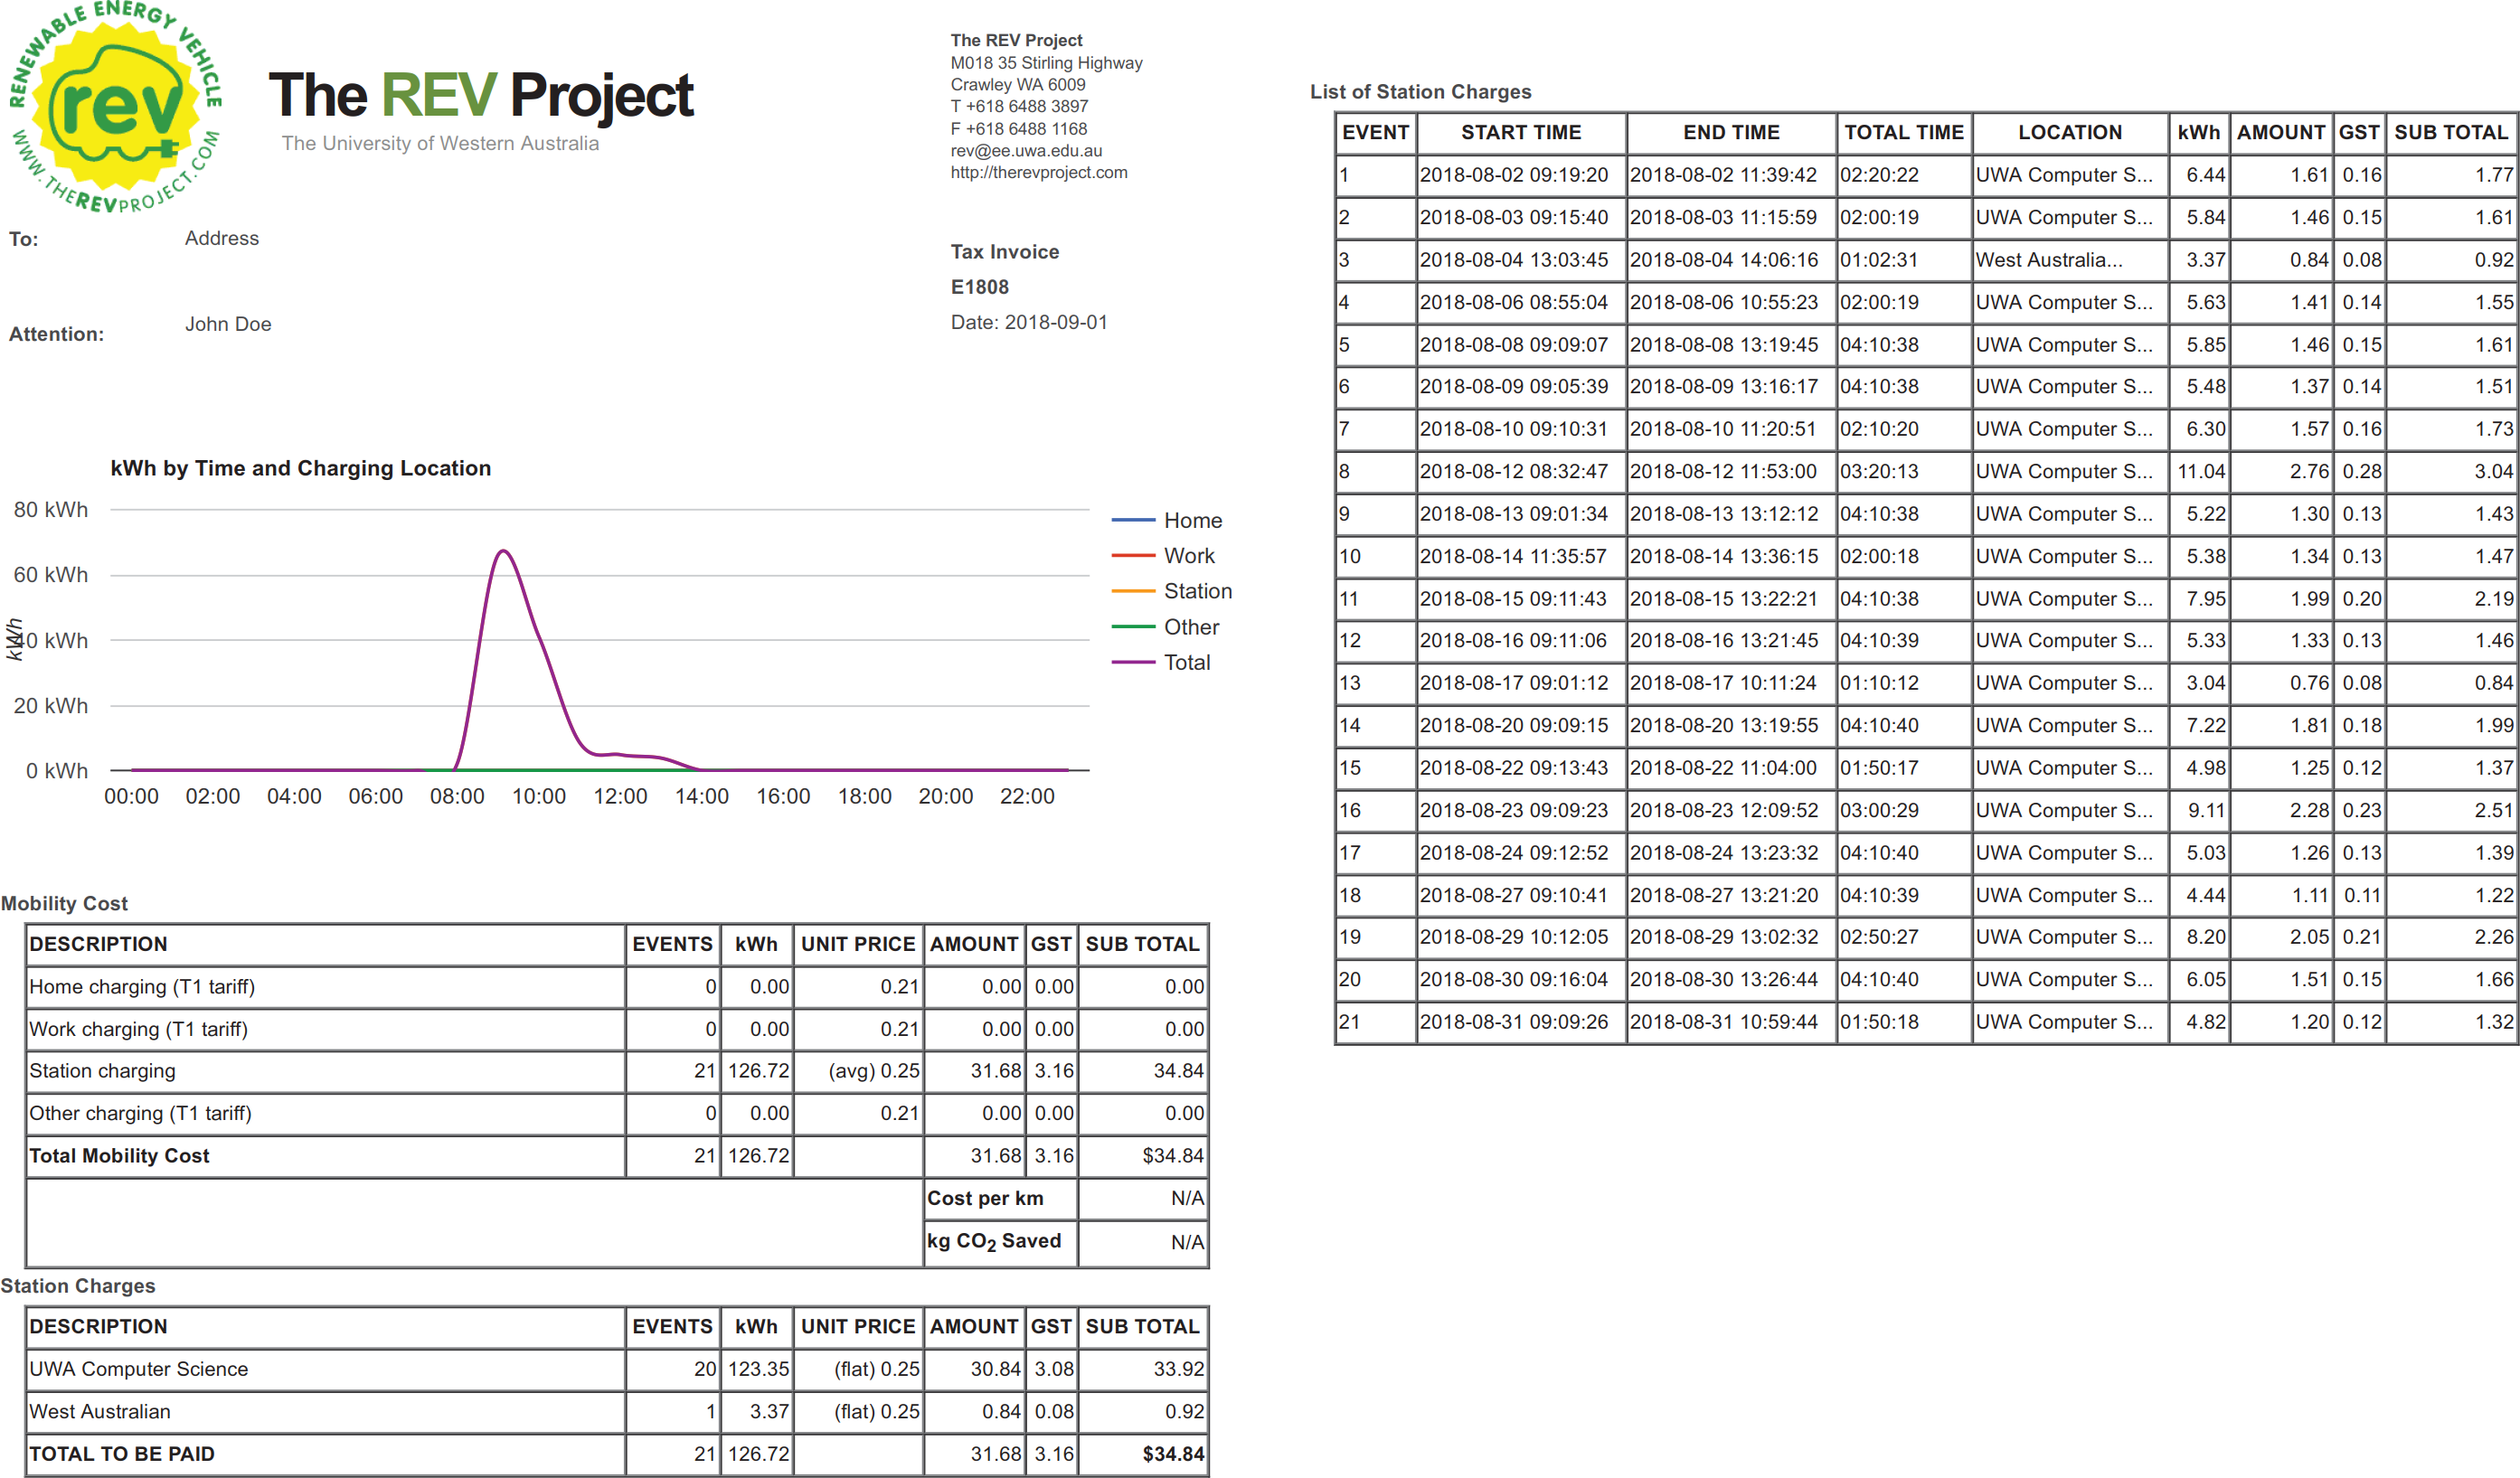
\includegraphics[width=\linewidth]{bill-user_1_crop}
	\caption{Itemised bill generated for a station user for August 2018.}
	\label{fig:9:uib}
\end{figure}

The line graph illustrates the cumulative charging energy consumption per hour for the vehicle according to the charging places from Section~\ref{sec:9:vt:db}, which is individually labelled as different coloured lines. The data used is summed through the per-hour energy usage data obtained in the query as mentioned in the first paragraph. To achieve this, the system uses an incremental function to individually increment the energy consumption for each location type at each hour of the day. 

The mobility cost is the first table presented following the line graph, which tabulates the cost of charging based on the user's charging location. Headers are given as the charging locations, number of events per location, energy consumption in kWh, tariff units and totals with GST, which is calculated as 10\% of the total price. We use a standard tariff of 25 cents per kWh for charging stations and 21 cents per kWh for other locations. When presented for a tracked fleet vehicle, it also calculates the cost per kilometres travelled and the amount of CO\textsubscript{2} saved. 

\nomenclature[z-gst]{GST}{Goods and services tax}

The second table presents station charges using the same headers found in the first table, which itemises the charging cost according to the charging stations used, detailing the individual station charging events found there. 

The third table further itemises the second one by listing each charging event of that vehicle on charging stations, listing each event using headers that correspond to its starting and ending timestamps, duration, station location, energy consumption, and amount totals with GST.

\subsection{Station Operator Billing}
Bills are also sent to station operators to summarise the monthly usage of their charging stations. Station operator bills consist of a community comparison, a line graph and an itemised table (see Fig.~\ref{fig:9:sob}). Data is obtained from the \texttt{station\_charges} table through a query that returns the charging user, starting and ending timestamps, energy consumption, per-hour charging and maintaining energy consumption, charging duration and connector side (left or right). 

\begin{figure}[H]
	\centering
	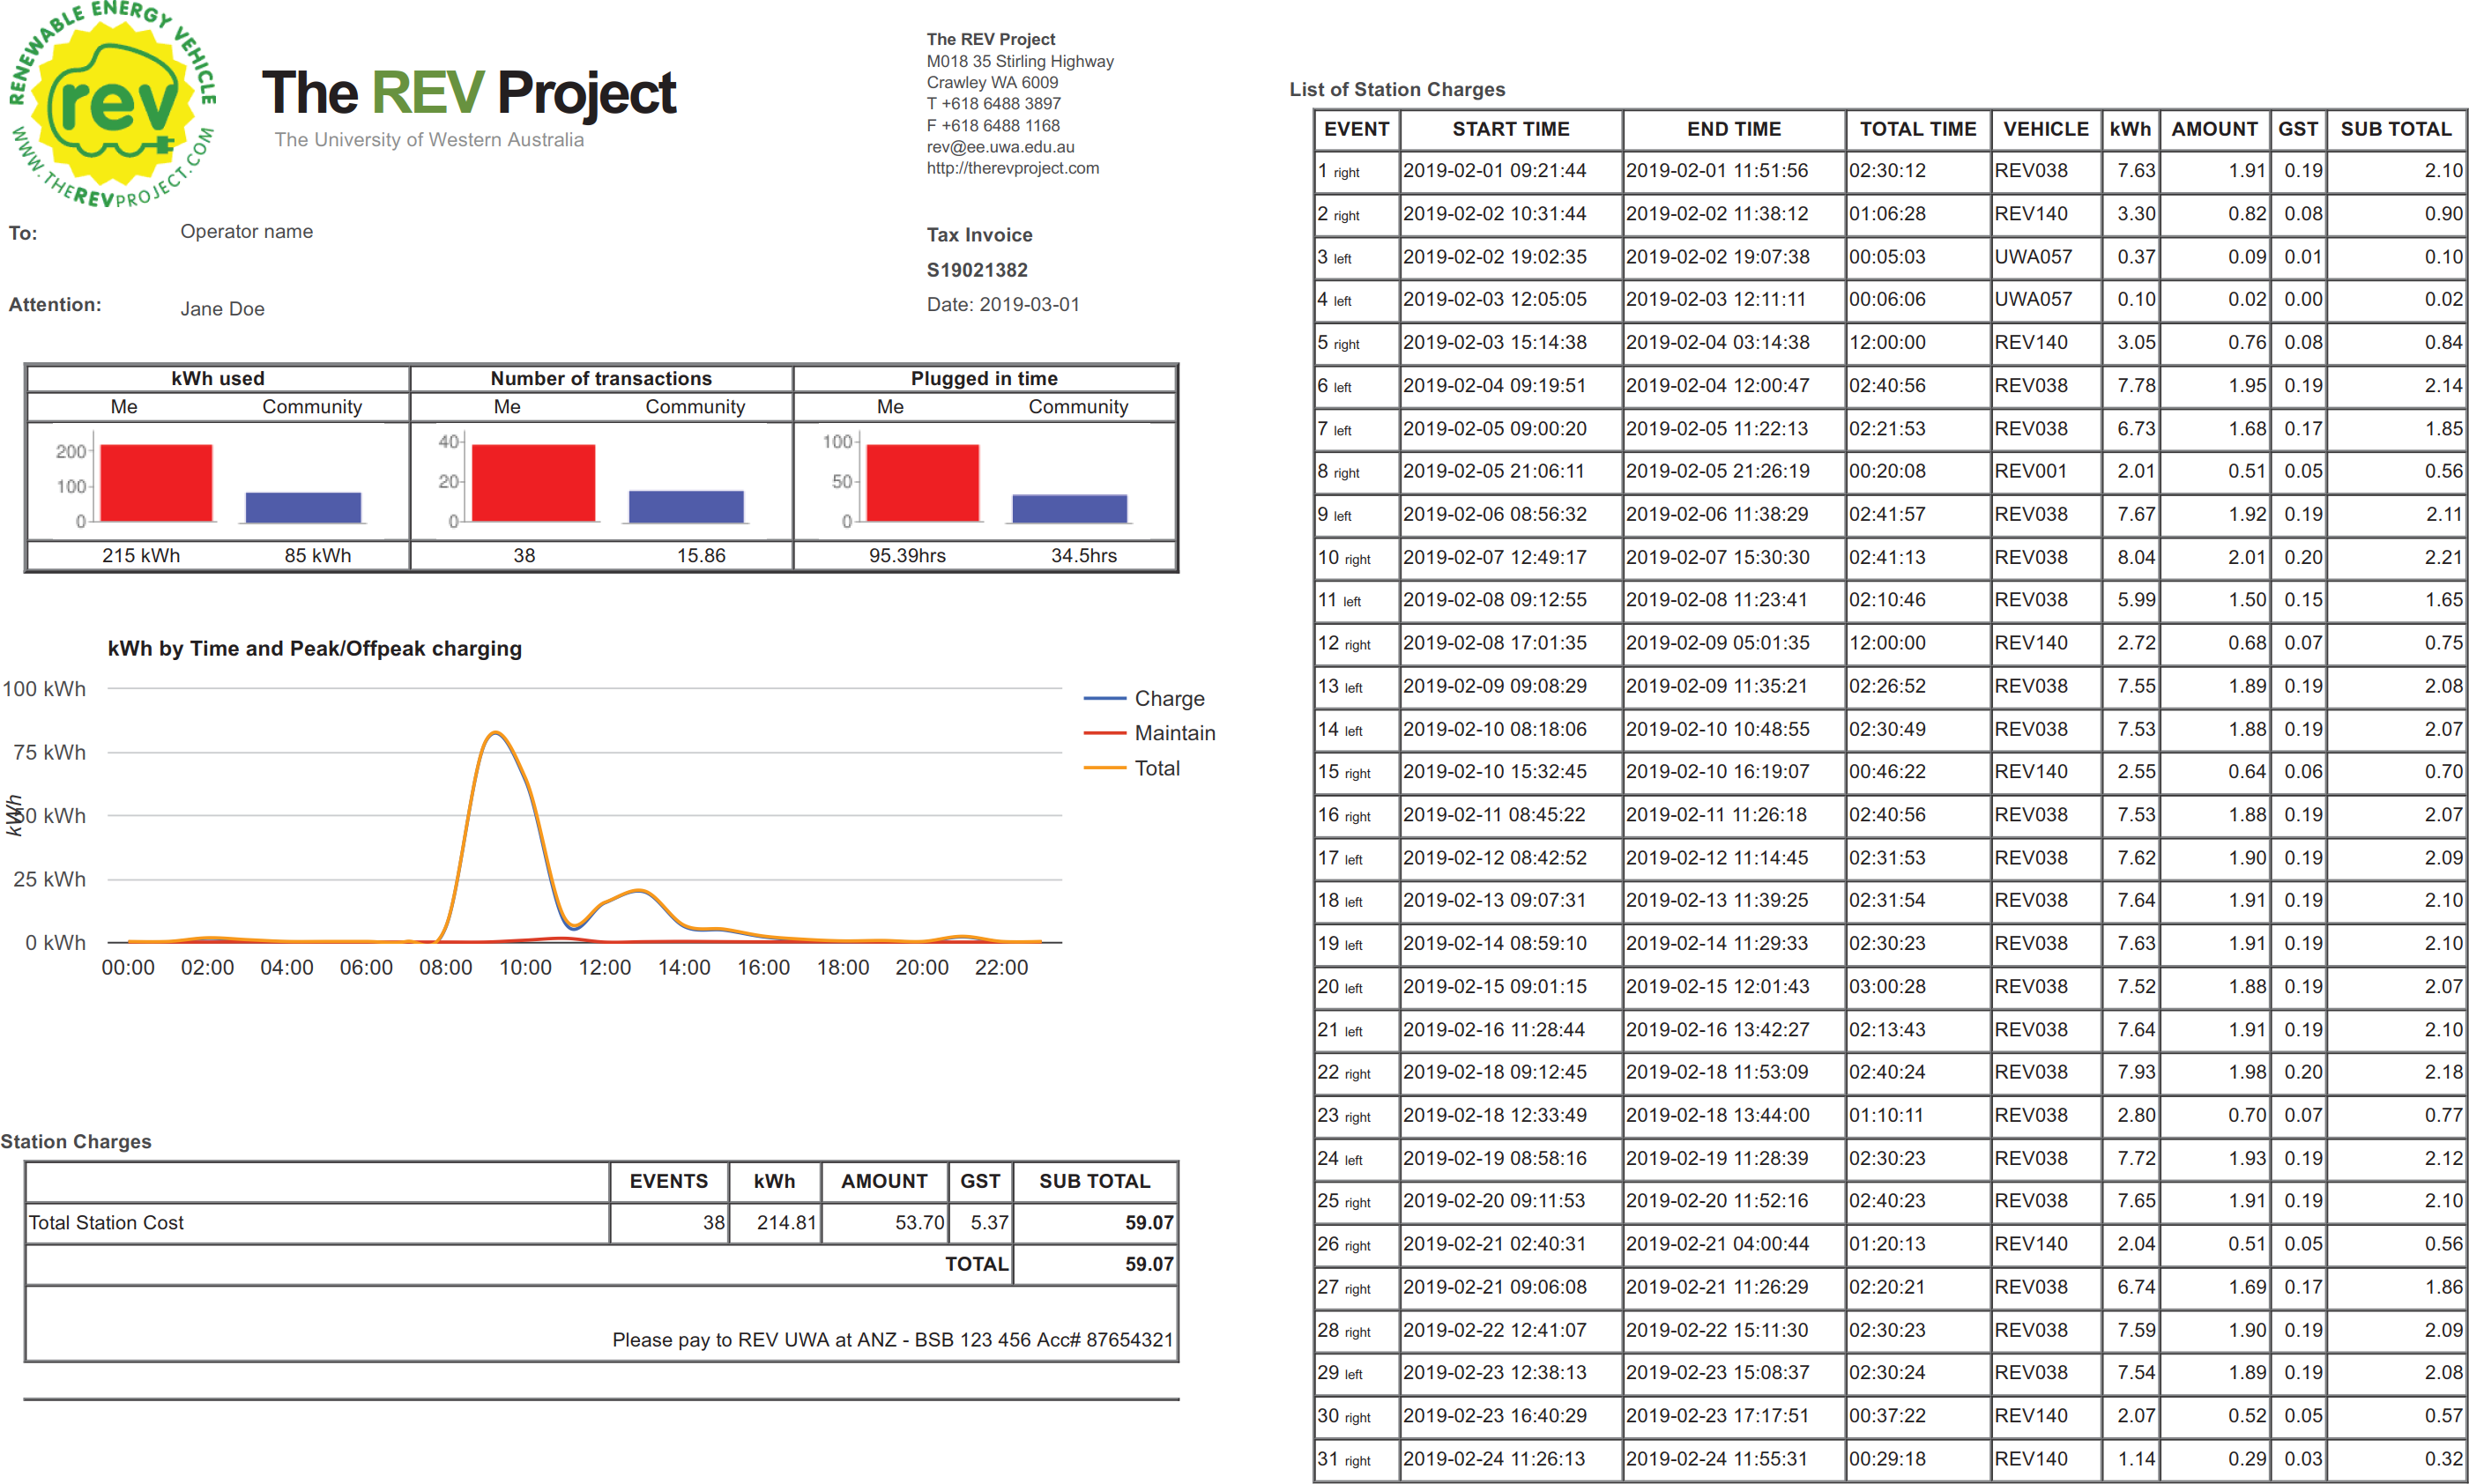
\includegraphics[width=\linewidth]{bill-station_1_crop}
	\caption{Itemised bill generated for station operators for February 2019.}
	\label{fig:9:sob}
\end{figure}

Community comparisons are drawn through the billing station against the average charging parameters of the other charging stations, where these parameters are given as their energy consumption in kWh, number of transactions and plugged in time. These are illustrated as a pair of colour bar charts for each parameter.

The line graph plots the per-hour energy consumption of the charging station on an average day, separated by its charging, maintaining and total plots. The total plot is the instantaneous sum of the “charge” and “maintain” energy consumption per hour. 

Finally, the \texttt{station\_charges} table begins by listing the total operating cost for the selected billing period, which lists the number of charging events and total energy consumption for that period, followed by the total energy costs on a 25 cents per kWh tariff. Another table chronologically itemises each charging event under the headers: connector side, starting and ending timestamps, charging duration, vehicle tag, energy consumption and charging price with GST.

\subsection{Network Overview}
REView displays an overview of the charging station network and vehicle's usages, which is accessible only to project administrators. This bill is generated for a selected period through a drop-down menu that evokes a query that produces a usage summary for our entire AC charging station network. Data on the network overview bill is presented as a line graph that is followed by two tables (see Fig.~\ref{fig:9:sum}). Data for this bill is obtained through a query that returns individual events under the following headers: station name, vehicle tag, energy consumption and per-hour energy usage (charging and maintaining charge). 

\begin{figure}[H]
	\centering
	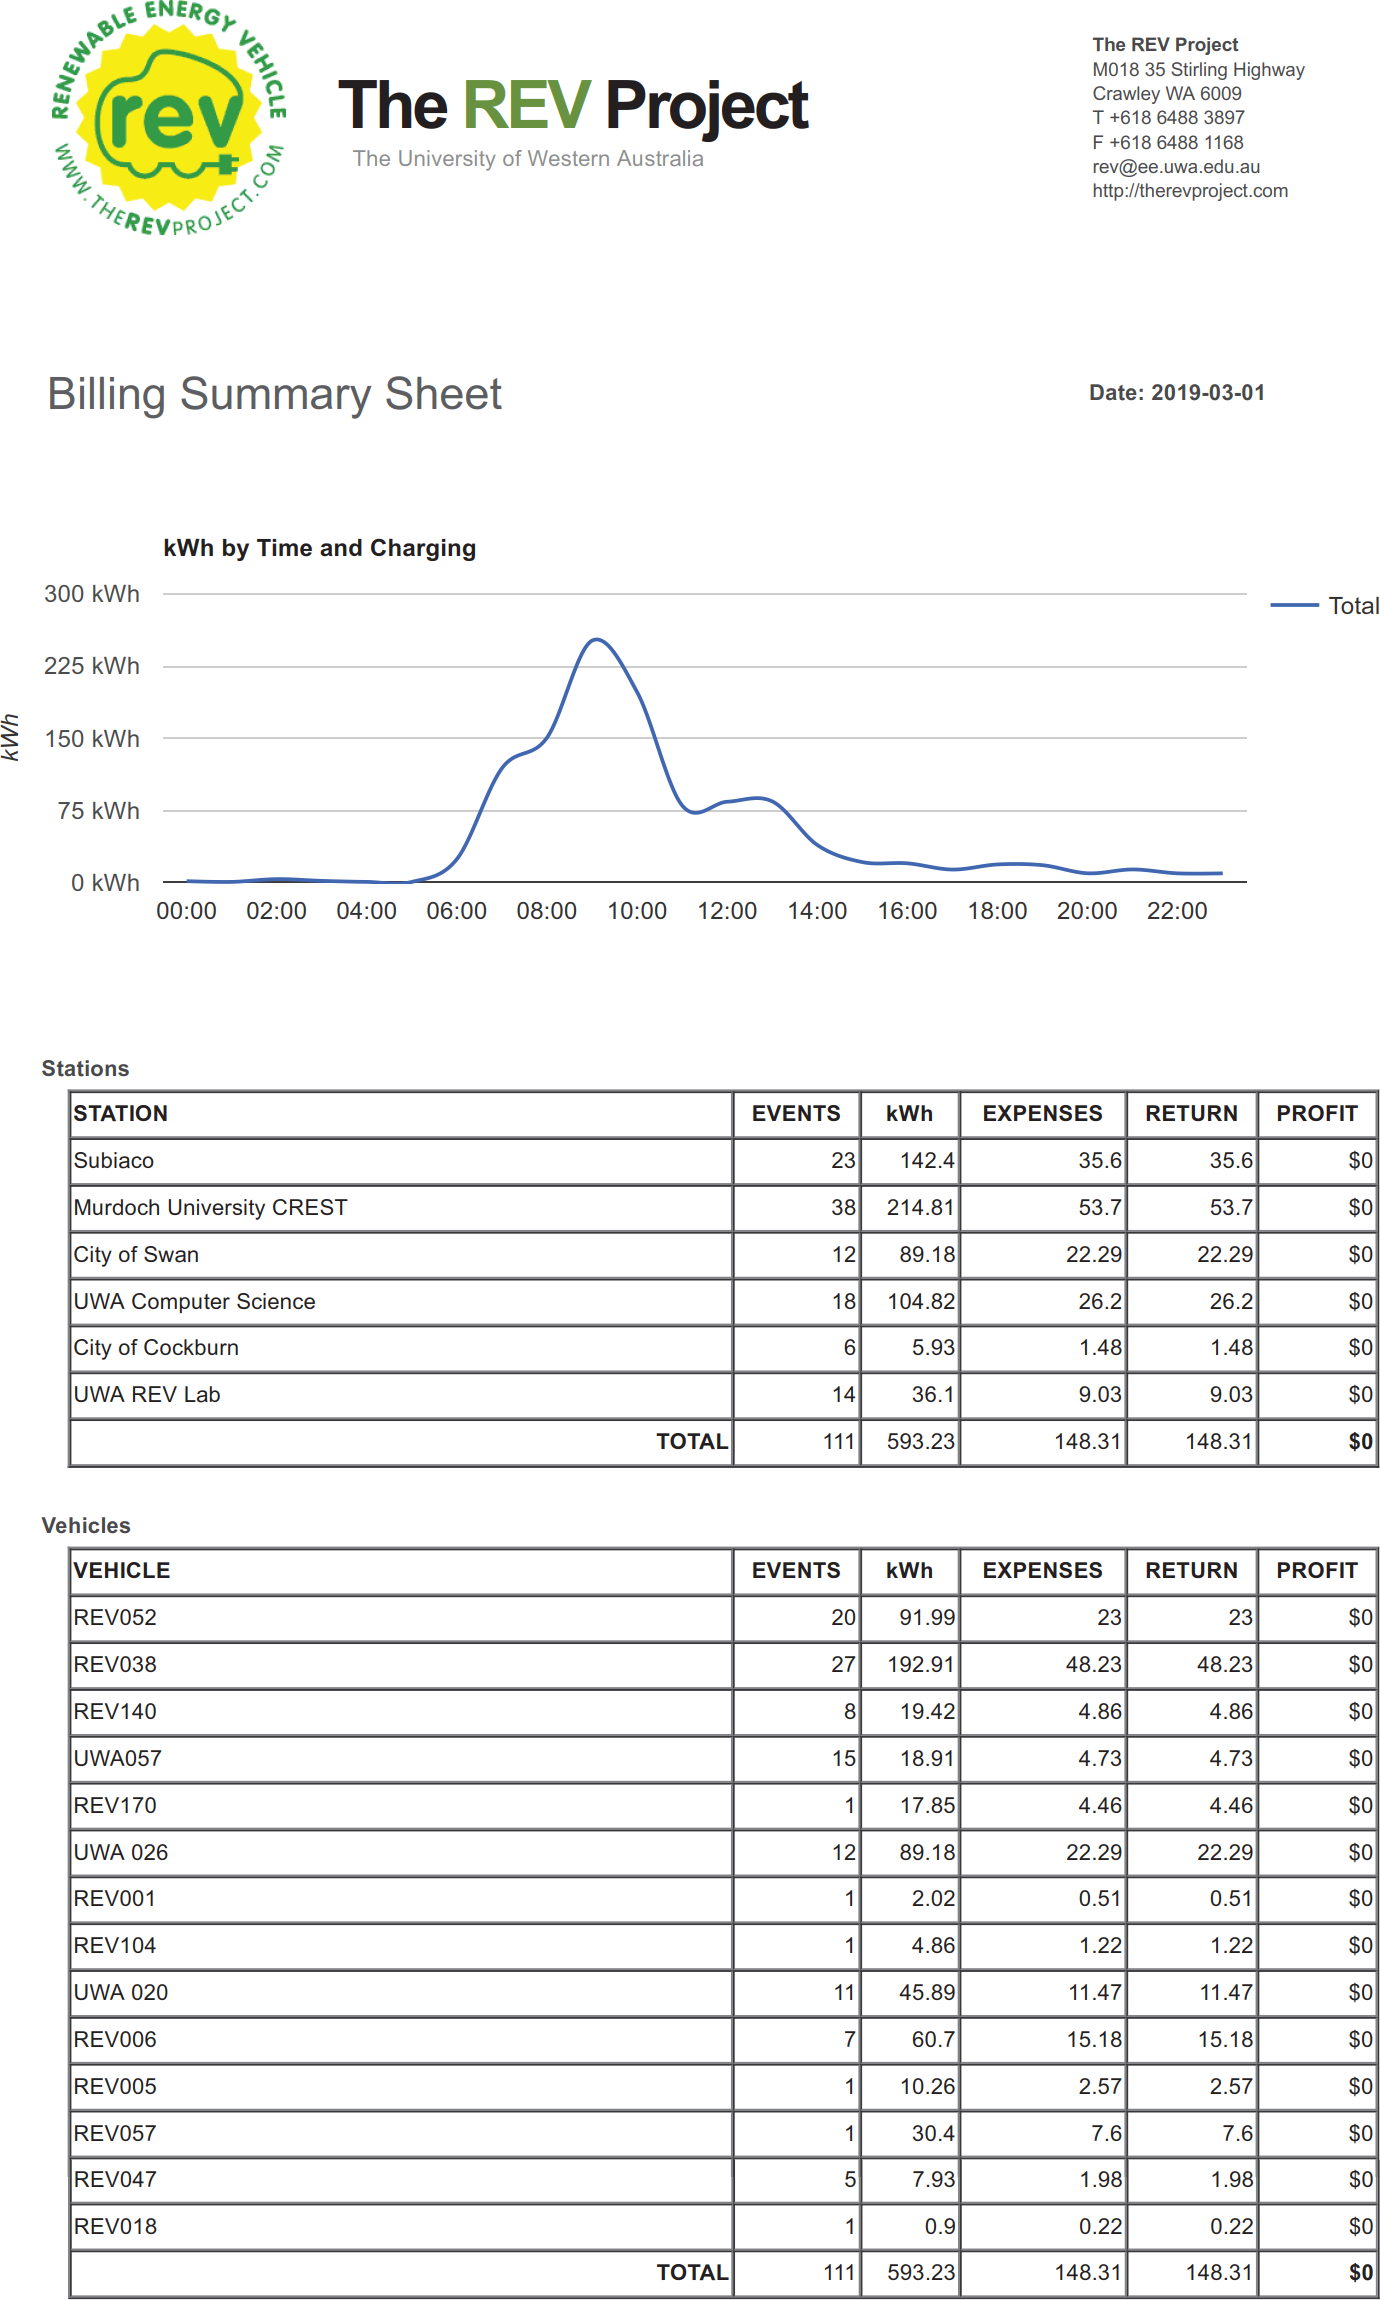
\includegraphics[width=0.5\linewidth]{bill-sum_1_crop}
	\caption{Network overview bill generated for March 2019.}
	\label{fig:9:sum}
\end{figure}

The line graph plots the cumulative per-hour energy usage across all stations for each hour of the day. This graph consolidates data under the per-hour energy usage header from the query, adds the energy usage for charging and maintaining charge across each hour of the day, and subsequently presents it as a sum of energy consumption for each event in the selected period. 

Each of the two tables aggregate charging events, one for the charging stations, and the other for the vehicles. These tables tabulate, for each charging station or vehicle, its number of charging events and total energy consumption in kWh. Additionally, this bill also includes cost (expenses), revenue (return) and profit generated from each event. (At the time of writing, our expenses and return tariffs are equally set as we are operating on a non-profit model). Data from the query is processed through a PHP back end that calculates values for an aggregated number of events and energy usage, as well as its associated costs. For each charging station and vehicle, an incremental function finds and increments the number of events and its associated energy usage, and subsequently its operating costs, revenues and profits, before encoding the entire table as a JSON representation.

\section{Mobile Application}
\label{sec:9:app}
REView has two mobile phone applications for EV drivers and station users as illustrated in Fig.~\ref{fig:9:app}. The first allows users to view their vehicle status on their mobile phone, showing location, status and battery level. The second allows station user s to see if their vehicle is still drawing power or if their EV is fully charged. It also allows users to check remotely if a station is occupied or free, allowing EV drivers to plan their trip ahead. These applications helped ease ‘range anxiety’ where drivers fear their vehicle will not have enough energy left in the battery to make it to a destination.

\begin{figure}[H]
	\centering
	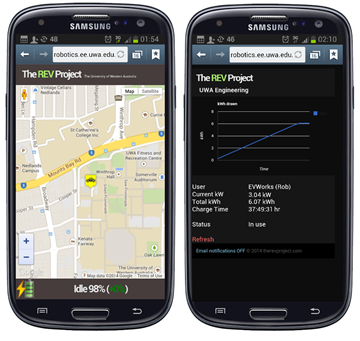
\includegraphics[width=0.7\linewidth]{smartphone}
	\caption{Smartphone application running REView.}
	\label{fig:9:app}
\end{figure}

Designing mobile web pages instead of apps makes sure they can be used for every smartphone or tablet model. The pages were developed as lightweight web pages using HTML 5 and JavaScript, which communicate periodically with the server for data updates. Each of the charging stations are listed in a page, with their availability indicated by a blue or green icon.

\section{Results}
\label{sec:9:results}
In this section, we will discuss results from the WA Electric Vehicle Trial, represented in REView graphs. We also present usage analyses and forecasts for the charging infrastructures.

\subsection{Overall Energy Usage}
Fig.~\ref{fig:9:overalle} shows the energy consumed charging EVs by hour of day and location. This information can be used for analysing EV grid impacts and the usage of renewable energy. The locations are defined as followed:
\begin{itemize}
	\item Home: A residential area.
	\item A commercial or industrial area.
	\item An EV charging station.
	\item An undefined area.
\end{itemize}

\begin{figure}[H]
	\centering
	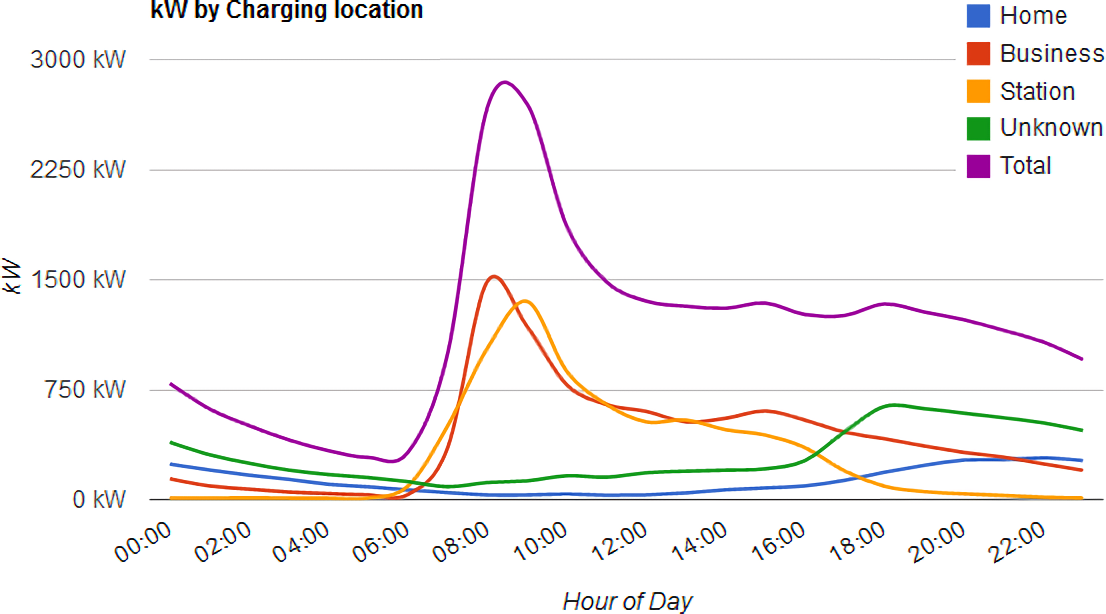
\includegraphics[width=0.8\linewidth]{overalle}
	\caption{Power drawn by hour of day for EV charging at various location types.}
	\label{fig:9:overalle}
\end{figure}

The peak of the energy supplied for charging vehicles (averaged over all locations) is during the morning hours around 9--10 am. This means, EVs are commuting from home to work and use a charging facility at work (most likely free of charge). It is worth noting that the majority of energy supplied is during sunshine hours especially for station charging and business charging. For unknown and home charging, there is a much smaller peak at around 6 pm, as vehicles are returning home and charging there. This also suggest that the majority of unknown locations are unlabelled home locations.

From this information and solar information gathered (see Fig.~\ref{fig:9:ac2hours1}) we can show that typical charging scenarios can be offset almost ideally by solar technology. Most of the charging occurs during the day, which differs fundamentally from the scenario propagated by some energy suppliers, which shows all EVs charging around 6pm when they return to home. 

\subsection{Charging Infrastructure Usage}
The statistics in this subsection are taken from REView’s Stations page showing the summary of all charging stations as a part of the WA Charging Station Network, from the beginning in June 2012 through March 2019.

In Figs.~\ref{fig:9:ac2kwh1}~and~\ref{fig:9:ac2hours1} we discuss the difference between charging and maintaining charge. It is common that an EV charger will draw a large amount of power until the battery pack is full, at which point the charger will continue to draw power at a significantly lower rate. When drawing power at the lower rate the EV can be doing several things including maintaining the charge of the battery pack, pre-conditioning the interior of the vehicle with heating or cooling or maintaining the temperature of the battery pack to improve driving efficiency. To distinguish between charging at maintaining charge, we define a vehicle to be charging if it is drawing more than 1 kW of power; otherwise we define it as “maintaining”.

\begin{figure}[H]
	\centering
	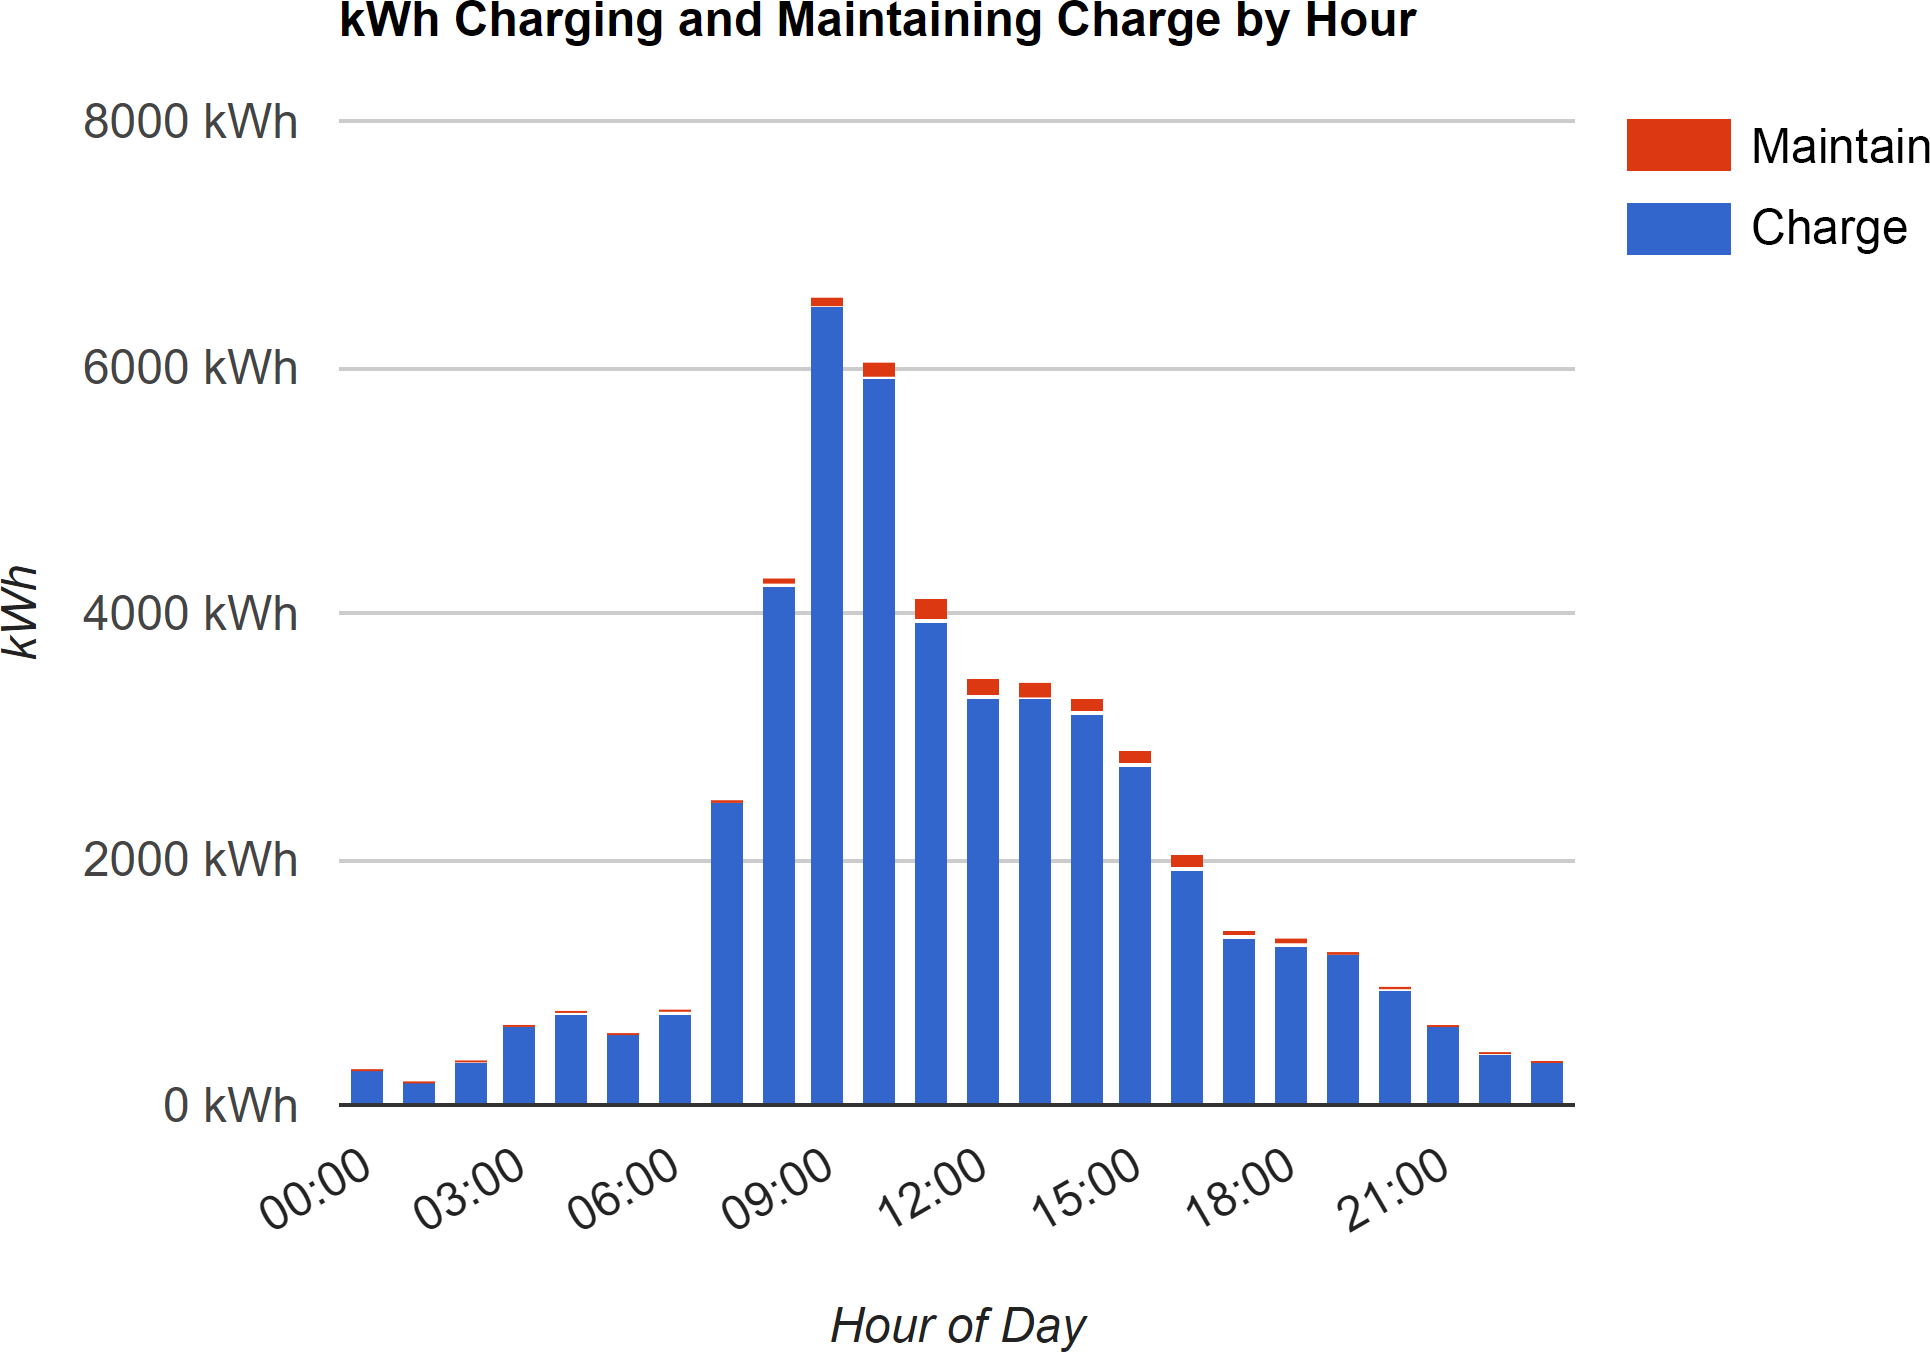
\includegraphics[width=0.8\linewidth]{ac2kwh1}
	\caption[Energy drawn by hour of day]{Energy drawn (in kWh) by hour of day stacked with power drawn for charging versus power drawn for maintaining charge.}
	\label{fig:9:ac2kwh1}
\end{figure}

\begin{figure}[H]
	\centering
	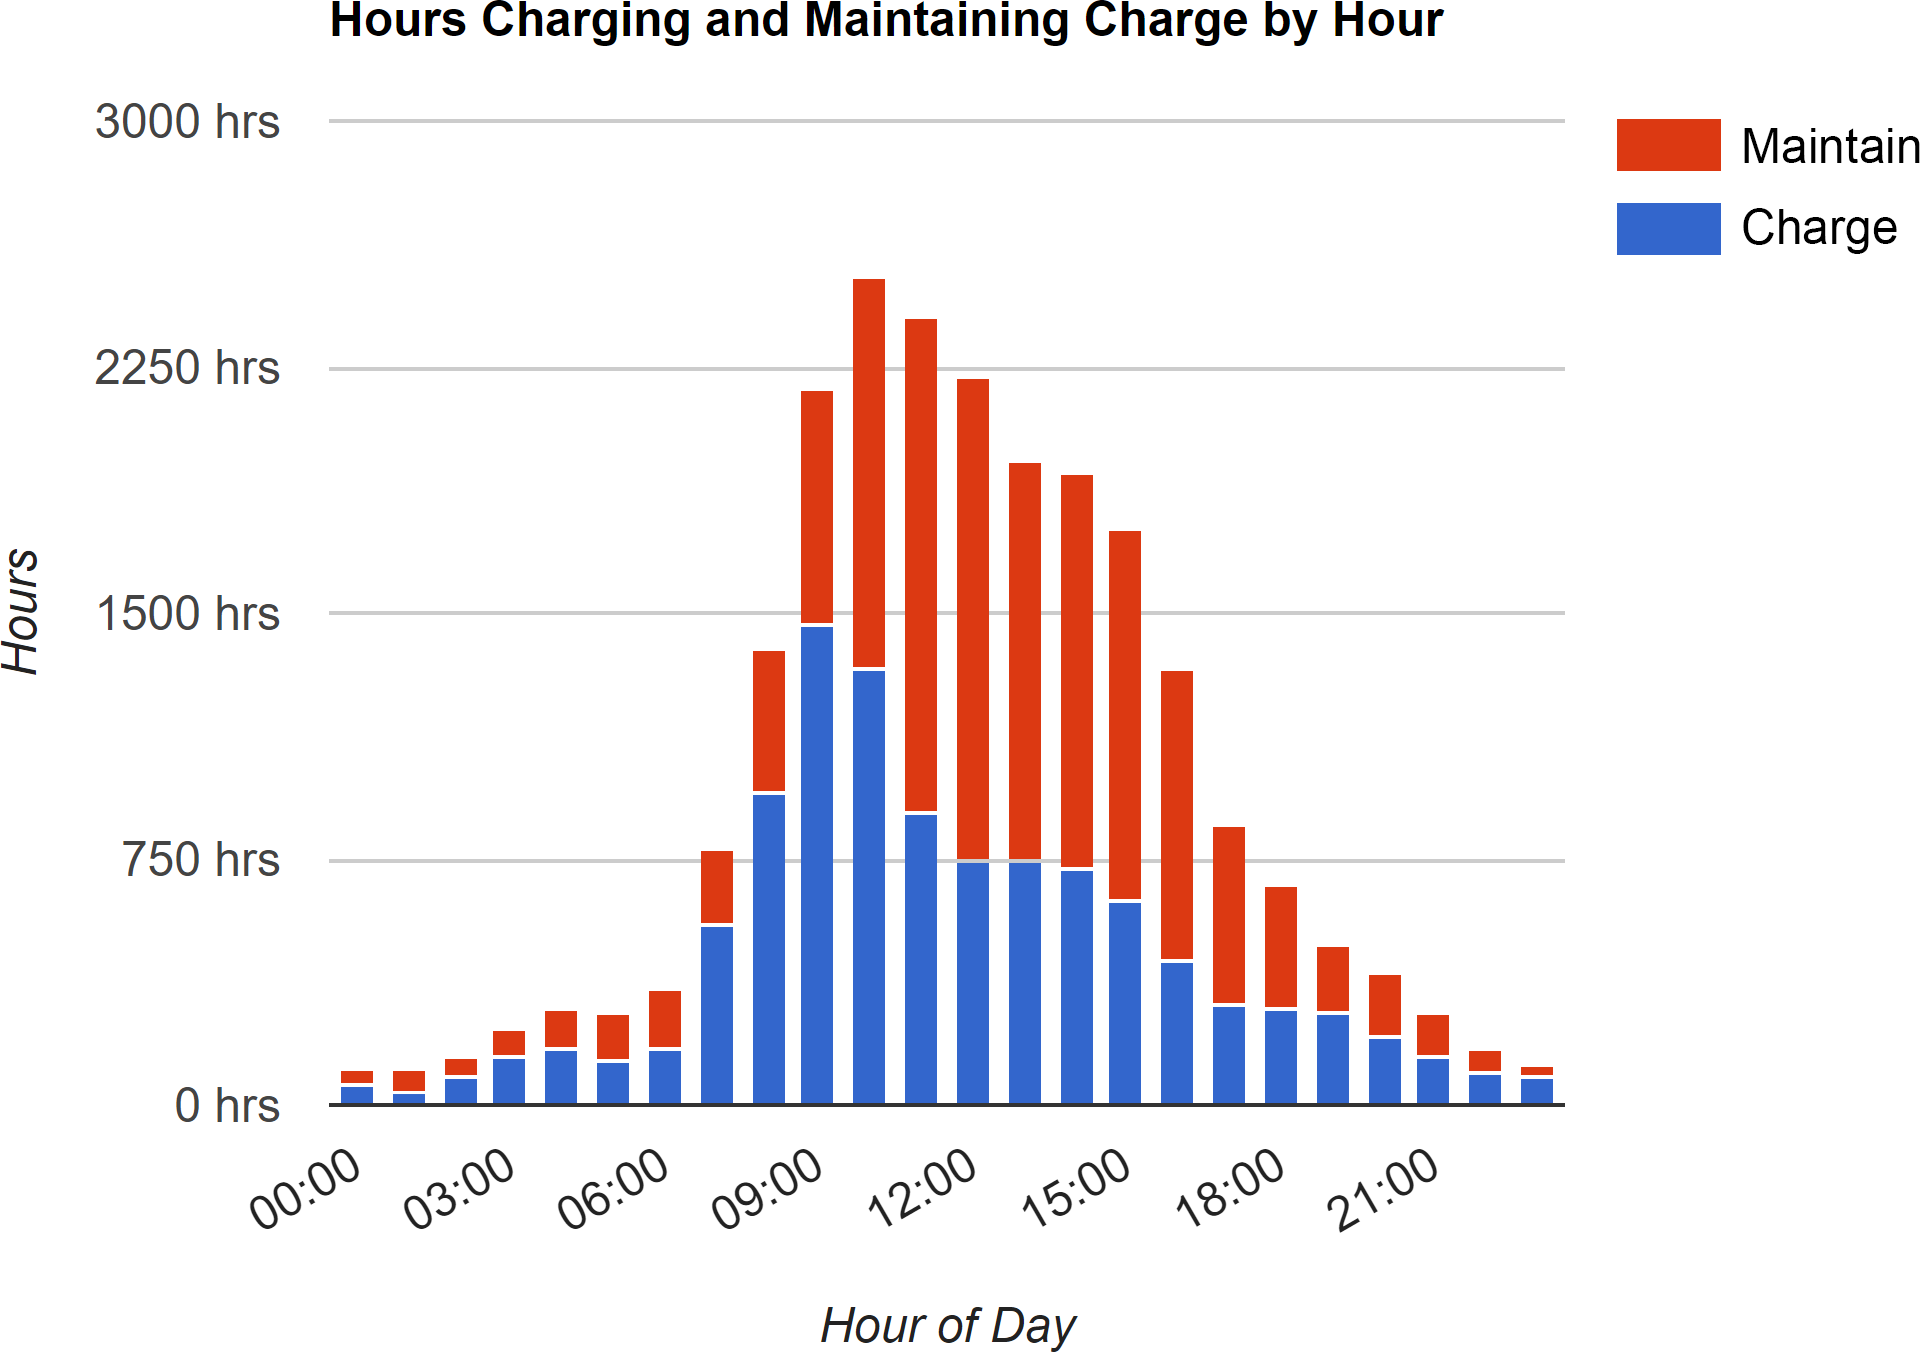
\includegraphics[width=0.8\linewidth]{ac2hours1}
	\caption[Amount of time spent at a charging station]{The amount of time spent (in hours) at a charging station with stacked charging time and maintaining charge time.}
	\label{fig:9:ac2hours1}
\end{figure}

From Fig.~\ref{fig:9:ac2kwh1} it is clear that throughout the day the majority of energy consumed from the station is done during a charging cycle. The energy for charging varies heavily depending on the time of day with the majority of energy being used throughout the day, reducing steadily into the evening and bottoming out around midnight. However, the maintaining charge energy consumption is similar in every hour throughout the day and night. This is because the electric vehicles are sometimes parked at the charging station overnight, and possibly over days when the EV is not being used. The maintaining charge consumption remains steady throughout the time the vehicle is idle.

In Fig.~\ref{fig:9:ac2hours1} we show the amount of time spent for charging and maintaining charge. From the discrepancy between the time required for charging and the time actually spent plugged in at the charging station, it can be seen that the charging stations in many cases are being misused as free parking locations for EVs. 

\begin{table}[H]
	\centering
	\caption{Charging station statistics June 2012 – March 2019 (81 months)}
	\label{tbl:9:css}
	\begin{tabular}{ll}
		\toprule
		Total kWh                          & 48788.343 kWh                     \\
		Estimated Cost (21.87¢ per kWh)    & \$10670.01                        \\
		Estimated Cost (peak/shoulder/off) & \$13891.92                        \\
		Number of Transactions             & 6917                              \\
		Plugged in Time                    & 957 days, 23:29:36                \\
		Charging Time                      & 444 days, 2:46:05 (46.36\%)       \\
		Maintaining Charge Time            & 513 days, 20:43:31 (53.64\%)      \\
		Avg Transaction Time               & 3:19:26                           \\
		Avg Charging Transaction Time      & 1:32:27 (46.36\%)                 \\
		Avg Maintaining Time               & 1:46:58 (53.64\%)                 \\
		Percentage time in use             & 3.21\%                            \\
		Power used in peak                 & 21785.22 kWh (44.65\%, \$9182.47) \\
		Power used in shoulder             & 21965.21 kWh (45.02\%, \$4709.34) \\
		Power used in off-peak             & 5037.91 kWh (10.33\%, \$570.29)   \\ \bottomrule
	\end{tabular}
\end{table}

Table~\ref{tbl:9:css} shows the summary of the charging station usage. From the information collected and automatically analysed, we can draw several conclusions. The flat rate plan of buying electricity is cheaper than the peak-shoulder-off peak plan. Only 46\% of the time spent at a station is used actually charging, while for the remaining 54\% of the time, the vehicle sits idle and blocks a charging station. This could allow for vehicle-to-grid technologies, however, as shown in~\cite{mullan_technical_2012}, V2G applications are not cost effective with current battery technology, as the addition wear and tear from extra charge cycles by far out-weighs the marginal energy cost. The stations themselves were only in use 3.2\% of the time logged, leaving a large proportion of the outlets idle. 

\subsection{Solar PV Monitoring}
In the graph in Fig.~\ref{fig:9:pv-day} we show the average hourly power output of the 20 kWp solar system at UWA for a typical summer day. The solar system begins generating energy at 6 am and shuts down at 6 pm, with the energy output peaking at 12 pm. The PV system generates approximately 80 kWh per day of operation. So, this system is generating around 30 MWh per year. In comparison, the 23 AC charging stations are using only 5.7 MWh per year on average (see Table~\ref{tbl:9:css}). This shows that one large solar PV installation can effectively power a number of EV charging stations. 

\begin{figure}[H]
	\centering
	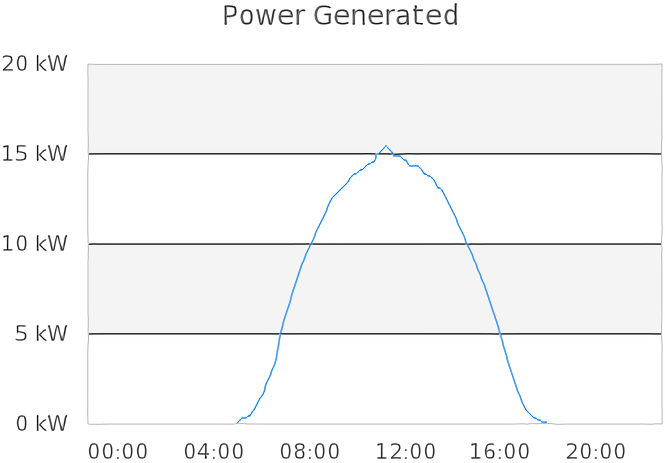
\includegraphics[width=0.8\linewidth]{pv_day}
	\caption[Average power output of UWA’s solar PV system]{Average power output for 20 kW of UWA’s solar PV system on a given day in February.}
	\label{fig:9:pv-day}
\end{figure}

\subsection{Heat Maps for EV Tracking}
With reference to Fig.~\ref{fig:9:vt-t-vis-hm}, we generated a heat map of the charging locations for tracked EVs from 2010 to July 2014. By looking at the charge events that took place during the day between 7 am and 6 pm, we can identify possible public locations in the Perth Metro area. The heat map shows several heavily utilised areas, including residential and business locations. One hot spot in Landsdale WA is the location of an EV conversion company that services most of the tracked EVs. From the heat map, we can determine that this is a place where a charging station would be highly frequented. The heat map also shows hot spots around most existing stations such as at The University of Western Australia.

\subsection{Charging Infrastructure Usage Forecast}
The historical data of the charging stations enables us to forecast the usage on these stations, and consequently predict the EV uptake rate in Western Australia. To achieve this, we have sampled data pertaining to charge frequencies $C$ and energy consumption $E$ for the AC charging network and the DC charging station. Data points were sampled from 1 December 2014 to 1 March 2019 (51 months) for DC charging, and from 1 June 2012 to 1 February 2019 (80 months) for AC charging.

\nomenclature[a-c]{$C$}{Number of charges} 
\nomenclature[a-e]{$E$}{Energy consumption} 

For both data sets, we conducted an augmented Dickey-Fuller test (ADF), which resulted in the rejection of the null hypothesis. This prompted us to fit the forecast over a logarithmic linear model using a log-level regression. We use a natural logarithm as the coefficients on its scale can be interpreted directly as approximate proportional differences, which we describe in our model interpretations.

\nomenclature[z-adf]{ADF}{Augmented Dickey-Fuller}

By modelling the usage of the DC charging station, we present our forecasts of its charging frequency and energy consumption, illustrated as graphs in Figs.~\ref{fig:9:dccountmodel} and~\ref{fig:9:dcenergymodel}. Note that these models do not account for any usage saturation for the stations, where given the average charge duration of three hours on an AC station and 24 minutes on the DC station, charging frequencies will saturate at 1800 charges per month for the DC station, and 240 charges per month for an AC station, assuming a back-to-back use case scenario, which is beyond the scope of the forecasts.

\begin{figure}[H]
	\centering
	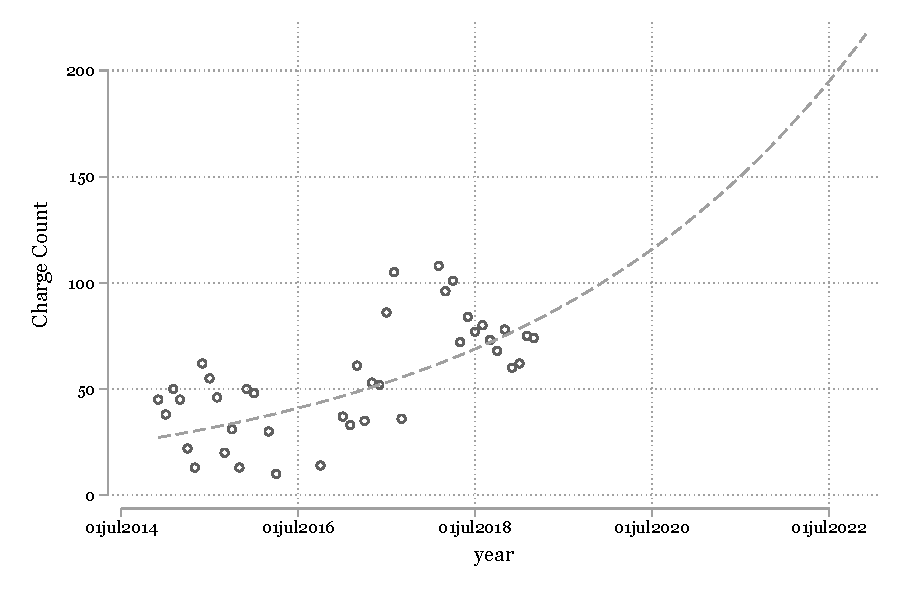
\includegraphics[width=0.9\linewidth]{DC_5_1}
	\caption[DC charge frequency regression model]{A regression model forecasting the per-month charge frequency on the DC charging station}
	\label{fig:9:dccountmodel}
\end{figure}

\begin{figure}[H]
	\centering
	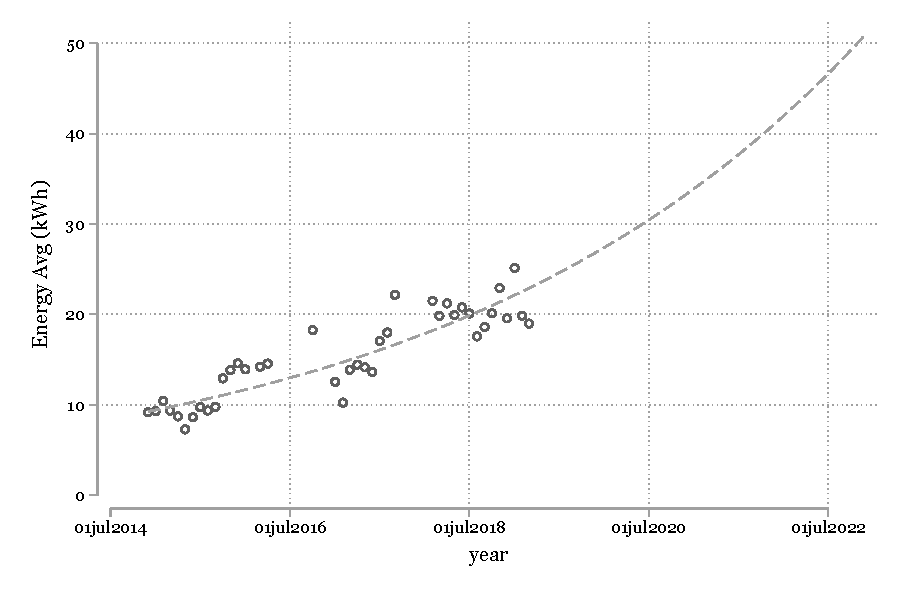
\includegraphics[width=0.9\linewidth]{DC_6_1}
	\caption[DC energy consumption regression model]{A regression model forecasting the per-month charging energy consumption per charge on the DC charging station.}
	\label{fig:9:dcenergymodel}
\end{figure}

The coefficients for the models are given as \eqref{eqn:9:cdc} for charge frequencies, and \eqref{eqn:9:edc} for energy consumption, with time $t$ measured per day:
\begin{align}
\ln(C_\mathrm{DC}) &= 0.0007116t - 10.9732 
\label{eqn:9:cdc} \\
\ln(E_\mathrm{DC}) &= 0.0005839t - 9.4866
\label{eqn:9:edc}
\end{align}
We can therefore infer from the coefficients that the charging frequency will increase by 0.07\% per day; the average energy consumption will increase by 0.05\% per day. This results in a 26.0\% annual increase in charge frequency, and a 21.3\% annual increase in energy consumption per charge. 

Similarly, we model our AC charging station network’s usage across the whole network as it compensates for the lower charging frequency on AC charging stations due to its longer charging duration. Here we present models for charging frequency and charging energy consumption as Figs.~\ref{fig:9:accountmodel} and~\ref{fig:9:acenergymodel}.

\begin{figure}[H]
	\centering
	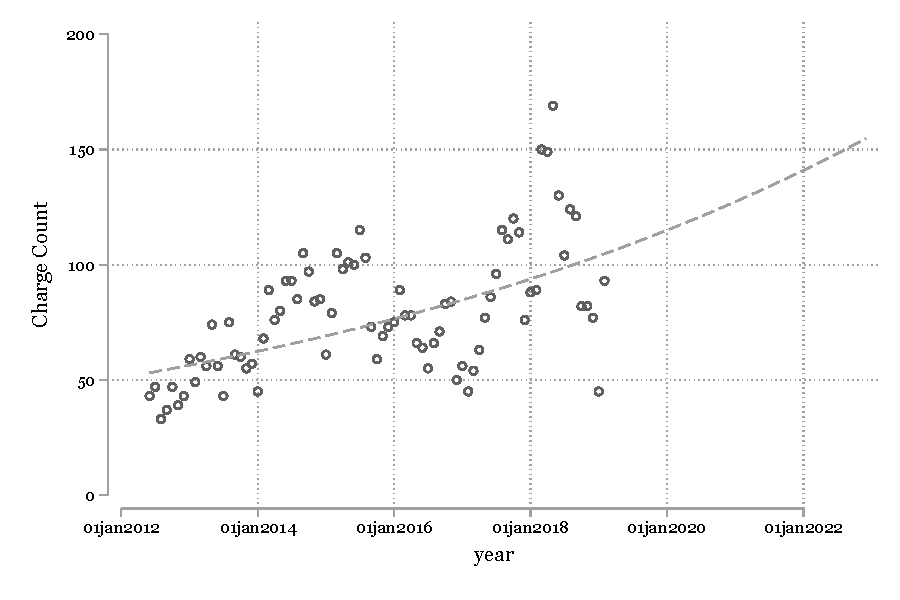
\includegraphics[width=0.9\linewidth]{AC_5_1}
	\caption[AC charge frequency regression model]{A regression model forecasting the per-month charge frequency on the AC charging network.}
	\label{fig:9:accountmodel}
\end{figure}

\begin{figure}[H]
	\centering
	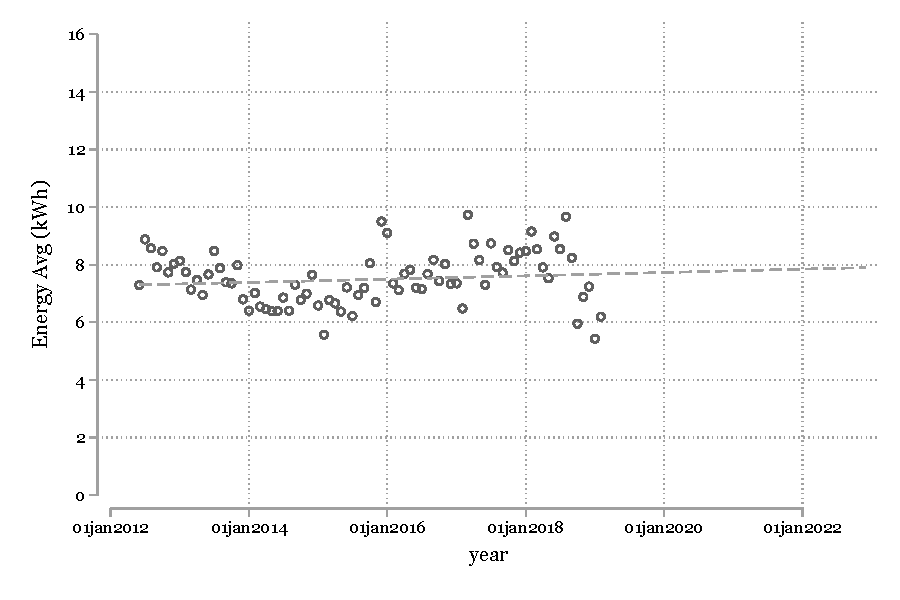
\includegraphics[width=0.9\linewidth]{AC_6_1}
	\caption[AC energy consumption regression model]{A regression model forecasting the per-month charging energy consumption per charge on the AC charging network.}
	\label{fig:9:acenergymodel}
\end{figure}

Likewise, the coefficients for the AC charging network’s models are given as \eqref{eqn:9:cac} for charge frequencies, and \eqref{eqn:9:eac} for energy consumption.
\begin{align}
\ln(C_\mathrm{AC}) &= 0.0002787t - 1.362995
\label{eqn:9:cac} \\
\ln(E_\mathrm{AC}) &= 0.0000206t - 1.592417
\label{eqn:9:eac}
\end{align}
From \eqref{eqn:9:cac}, we interpret the coefficients whereby the charging frequency for the AC network will increase by 0.03\% per day, or 10.2\% per annum; the average energy consumption per charge at an AC station increases by 0.002\% per day, or 0.75\% per annum. 

We can thus deduce though these models that DC charging is the more preferred charging method for local EVs, and that the increasing energy consumption per charge could suggest the increasing battery capacity and range for newer EVs. As the number of EV uptakes in WA increases, so does the charging frequency at the DC station. Note that we have observed different charging behaviours across AC and DC charging stations whereby our DC charging station registers more unique users, and many of the charging events registered large energy consumptions, as shown in Fig.~\ref{fig:9:energy-cons}. This likely implies that most users are charging their vehicle from a low charge state. On the contrary, most AC charging users are routine users, whereby the charging bays are occupied for extended periods while the driver is at work, for example. This explains the low increase in energy consumption across AC charges, as charging events are often top-up charges that recharge the vehicle after a daily commute, and where the vehicle is unlikely to be at a low charge state. However, the increase in charge frequency on the AC network also implies the increasing EV uptake in WA.

\begin{figure}[H]
	\centering
	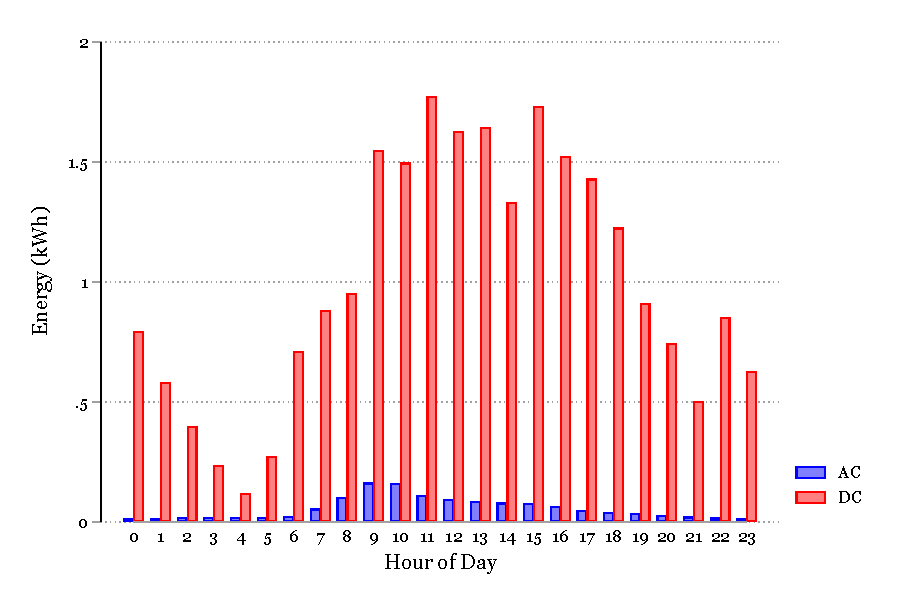
\includegraphics[width=\linewidth]{energy_consumption}
	\caption{Per-hour energy usage comparison between AC and DC charging stations.}
	\label{fig:9:energy-cons}
\end{figure}

\section{Conclusion}
\label{sec:9:conclusion}
We have presented in this paper our telematics platform for connected electric vehicles and its infrastructures, REView. This system comprises live data information portals for customers as well as for fleet operators and charging network operators. It provides statistical information on time and location of charge events and includes a time-of-use billing system. It interfaces with charging stations, vehicle-based data loggers and solar PV systems. This required configuration and testing for each of the different devices in parallel with server and database development. The software was written for server-based and client-based processing and data display. Each of the different levels of this project (server, data processing, and interface) was developed in tandem to ensure integration. The software was designed in a modular way with separate scripts for individual features, making unit testing easier, reducing integration problems and isolating failures. All of the programming languages used in the system are interpreted, which means that design changes could be made very quickly. The main contribution of REView is that it consolidates incoming data from connected vehicle fleets, charging stations and power generators into a unified platform to improve the efficiency of information presentation. These are presented entirely as a web-based solution for increased accessibility and are supplemented by additional features such as billing which supports the monetisation of the system. From the data collected and analysed, we can deduce that solar technology is an effective way for offsetting energy required for charging EVs at public charging stations and place-of-work. For home charging, energy is mostly required outside of solar generation hours and would need to be provided by a domestic energy storage system. A 20 kW solar PV system was more than enough to offset the energy used by EV charging at 23 public charging stations. The results produced from this system has, throughout the years, enabled us to perform various analyses on the EV landscape within Western Australia. 

Moving forward, with the increase of data volume and infrastructures, future plans for REView will involve its eventual compliance with the arrival of the Internet of Vehicles (IoV) standards. With this proposal, we are planning to integrate REView as a cloud application while utilising the Platform as a Service (PaaS) environment. This will enable us to streamline further developments on REView and to increase its modularity through more efficient workflows while improving scalability.

\nomenclature[z-paas]{PaaS}{Platform as a Service}
